\RequirePackage{lineno}
\documentclass[aps,prd,twocolumn,showpacs,superscriptaddress,nofootinbib,floatfix,letterpaper]{revtex4-1}
\pdfoutput=1
\usepackage{placeins}
\usepackage{multirow}
\usepackage[utf8]{inputenc}
\usepackage{color}
\usepackage[caption=false]{subfig}
\usepackage{xspace}
\usepackage{graphicx}
\usepackage[pdftex,bookmarks,hidelinks]{hyperref}
\usepackage{amsmath}

\graphicspath{ {graphics/} }

\newcommand{\numu}{\ensuremath{\nu_\mu}\xspace}
\newcommand{\nue}{\ensuremath{\nu_e}\xspace}
\newcommand{\nutau}{\ensuremath{\nu_\tau}\xspace}
\newcommand{\anumu}{\ensuremath{\bar\nu_\mu}\xspace}
\newcommand{\anue}{\ensuremath{\bar\nu_e}\xspace}
\newcommand{\anutau}{\ensuremath{\bar\nu_\tau}\xspace}

\newcommand{\dm}[1]{\ensuremath{\Delta m^2_{#1}}\xspace} % example: \dm{12}
\newcommand{\sinst}[1]{\ensuremath{\sin^2\theta_{#1}}\xspace} % example \sinst{12}
\newcommand{\sinstt}[1]{\ensuremath{\sin^22\theta_{#1}}\xspace}  % example \sinstt{12}
\newcommand{\deltacp}{\ensuremath{\delta_{\rm CP}}\xspace}   % example \deltacp

\newcommand{\numutonumu}{\ensuremath{\numu\rightarrow\numu}\xspace}
\newcommand{\numutonue}{\ensuremath{\numu\rightarrow\nue}\xspace}

\newcommand{\numubartonumubar}{
\ensuremath{\overline{\numu}\rightarrow\overline{\numu}}\xspace
}

\newcommand{\numubartonuebar}{
\ensuremath{\overline{\numu}\rightarrow\overline{\nue}}\xspace
}

\newcommand{\todo}[1]{\textcolor{blue}{#1}}
\newcommand\addcite{[{\color{blue} \underline{CITATION NEEDED}}]~}
\def\bracketbar{\hbox{\kern-8pt\raise1pt%
    \hbox{{\tiny(}{\lower1.5pt\hbox{\bf--}}{\tiny)}}}}
\newcommand{\dchisq}{\ensuremath{\Delta\chi^{2}}\xspace}
\newcommand{\dchisqcrit}{\ensuremath{\Delta\chi^{2}_{c}}\xspace}

\begin{document}

\title{Low exposure long-baseline neutrino oscillation sensitivity of the DUNE experiment}
\date{\today}
\collaboration{DUNE Collaboration}
\noaffiliation
% %----------------------------------------------------
% List of institutions, need not be alphabetical
% Need to also add institution as \affiliation below this to get alphabetical order right
\newcommand{\Abilene}{Abilene Christian University, Abilene, TX 79601, USA}
\newcommand{\Albanysuny}{University of Albany, SUNY, Albany, NY 12222, USA}
\newcommand{\Amsterdam}{University of Amsterdam, NL-1098 XG Amsterdam, The Netherlands}
\newcommand{\Antalya}{Antalya Bilim University, 07190 D{\"o}{\c{s}}emealt{\i}/Antalya, Turkey}
\newcommand{\Antananarivo}{University of Antananarivo, Antananarivo 101, Madagascar}
\newcommand{\AntonioNarino}{Universidad Antonio Nari{\~n}o, Bogot{\'a}, Colombia}
\newcommand{\Argonne}{Argonne National Laboratory, Argonne, IL 60439, USA}
\newcommand{\Arizona}{University of Arizona, Tucson, AZ 85721, USA}
\newcommand{\Asuncion}{Universidad Nacional de Asunci{\'o}n, San Lorenzo, Paraguay}
\newcommand{\Athens}{University of Athens, Zografou GR 157 84, Greece}
\newcommand{\Atlantico}{Universidad del Atl{\'a}ntico, Barranquilla, Atl{\'a}ntico, Colombia}
\newcommand{\Augustana}{Augustana University, Sioux Falls, SD 57197, USA}
\newcommand{\Banaras}{Banaras Hindu University, Varanasi - 221 005, India}
\newcommand{\Basel}{University of Basel, CH-4056 Basel, Switzerland}
\newcommand{\Bern}{University of Bern, CH-3012 Bern, Switzerland}
\newcommand{\Beykent}{Beykent University, Istanbul, Turkey}
\newcommand{\Birmingham}{University of Birmingham, Birmingham B15 2TT, United Kingdom}
\newcommand{\BolognaUniversity}{Universit{\`a} del Bologna, 40127 Bologna, Italy}
\newcommand{\Boston}{Boston University, Boston, MA 02215, USA}
\newcommand{\Bristol}{University of Bristol, Bristol BS8 1TL, United Kingdom}
\newcommand{\Brookhaven}{Brookhaven National Laboratory, Upton, NY 11973, USA}
\newcommand{\Bucharest}{University of Bucharest, Bucharest, Romania}
\newcommand{\CBPF}{Centro Brasileiro de Pesquisas F\'isicas, Rio de Janeiro, RJ 22290-180, Brazil}
\newcommand{\CEASaclay}{IRFU, CEA, Universit{\'e} Paris-Saclay, F-91191 Gif-sur-Yvette, France}
\newcommand{\CERN}{CERN, The European Organization for Nuclear Research, 1211 Meyrin, Switzerland}
\newcommand{\CIEMAT}{CIEMAT, Centro de Investigaciones Energ{\'e}ticas, Medioambientales y Tecnol{\'o}gicas, E-28040 Madrid, Spain}
\newcommand{\CUSB}{Central University of South Bihar, Gaya, 824236, India }
\newcommand{\CalBerkeley}{University of California Berkeley, Berkeley, CA 94720, USA}
\newcommand{\CalDavis}{University of California Davis, Davis, CA 95616, USA}
\newcommand{\CalIrvine}{University of California Irvine, Irvine, CA 92697, USA}
\newcommand{\CalLosangeles}{University of California Los Angeles, Los Angeles, CA 90095, USA}
\newcommand{\CalRiverside}{University of California Riverside, Riverside CA 92521, USA}
\newcommand{\CalSantabarbara}{University of California Santa Barbara, Santa Barbara, California 93106 USA}
\newcommand{\Caltech}{California Institute of Technology, Pasadena, CA 91125, USA}
\newcommand{\Cambridge}{University of Cambridge, Cambridge CB3 0HE, United Kingdom}
\newcommand{\Campinas}{Universidade Estadual de Campinas, Campinas - SP, 13083-970, Brazil}
\newcommand{\CataniaUniversitadi}{Universit{\`a} di Catania, 2 - 95131 Catania, Italy}
\newcommand{\Catolica}{Universidad Cat{\'o}lica del Norte, Antofagasta, Chile}
\newcommand{\Charles}{Institute of Particle and Nuclear Physics of the Faculty of Mathematics and Physics of the Charles University, 180 00 Prague 8, Czech Republic }
\newcommand{\Chicago}{University of Chicago, Chicago, IL 60637, USA}
\newcommand{\ChungAng}{Chung-Ang University, Seoul 06974, South Korea}
\newcommand{\Cincinnati}{University of Cincinnati, Cincinnati, OH 45221, USA}
\newcommand{\Cinvestav}{Centro de Investigaci{\'o}n y de Estudios Avanzados del Instituto Polit{\'e}cnico Nacional (Cinvestav), Mexico City, Mexico}
\newcommand{\Colima}{Universidad de Colima, Colima, Mexico}
\newcommand{\ColoradoBoulder}{University of Colorado Boulder, Boulder, CO 80309, USA}
\newcommand{\ColoradoState}{Colorado State University, Fort Collins, CO 80523, USA}
\newcommand{\Columbia}{Columbia University, New York, NY 10027, USA}
\newcommand{\CzechAcademyofSciences}{Institute of Physics, Czech Academy of Sciences, 182 00 Prague 8, Czech Republic}
\newcommand{\CzechTechnical}{Czech Technical University, 115 19 Prague 1, Czech Republic}
\newcommand{\DakotaState}{Dakota State University, Madison, SD 57042, USA}
\newcommand{\Dallas}{University of Dallas, Irving, TX 75062-4736, USA}
\newcommand{\DannecyleVieux}{Laboratoire d{\textquoteright}Annecy de Physique des Particules, Univ. Grenoble Alpes, Univ. Savoie Mont Blanc, CNRS, LAPP-IN2P3, 74000 Annecy, France}
\newcommand{\Daresbury}{Daresbury Laboratory, Cheshire WA4 4AD, United Kingdom}
\newcommand{\Drexel}{Drexel University, Philadelphia, PA 19104, USA}
\newcommand{\Duke}{Duke University, Durham, NC 27708, USA}
\newcommand{\Durham}{Durham University, Durham DH1 3LE, United Kingdom}
\newcommand{\EIA}{Universidad EIA, Envigado, Antioquia, Colombia}
\newcommand{\ETH}{ETH Zurich, Zurich, Switzerland}
\newcommand{\Edinburgh}{University of Edinburgh, Edinburgh EH8 9YL, United Kingdom}
\newcommand{\FCULport}{Faculdade de Ci{\^e}ncias da Universidade de Lisboa - FCUL, 1749-016 Lisboa, Portugal}
\newcommand{\FederaldeAlfenas}{Universidade Federal de Alfenas, Po{\c{c}}os de Caldas - MG, 37715-400, Brazil}
\newcommand{\FederaldeGoias}{Universidade Federal de Goias, Goiania, GO 74690-900, Brazil}
\newcommand{\FederaldeSaoCarlos}{Universidade Federal de S{\~a}o Carlos, Araras - SP, 13604-900, Brazil}
\newcommand{\FederaldoABC}{Universidade Federal do ABC, Santo Andr{\'e} - SP, 09210-580, Brazil}
\newcommand{\FederaldoRio}{Universidade Federal do Rio de Janeiro,  Rio de Janeiro - RJ, 21941-901, Brazil}
\newcommand{\Fermi}{Fermi National Accelerator Laboratory, Batavia, IL 60510, USA}
\newcommand{\Ferrarauniv}{University of Ferrara, Ferrara, Italy}
\newcommand{\Florida}{University of Florida, Gainesville, FL 32611-8440, USA}
\newcommand{\Fluminense}{Fluminense Federal University, 9 Icara{\'\i} Niter{\'o}i - RJ, 24220-900, Brazil }
\newcommand{\Genova}{Universit{\`a} degli Studi di Genova, Genova, Italy}
\newcommand{\Georgian}{Georgian Technical University, Tbilisi, Georgia}
\newcommand{\GranSasso}{Gran Sasso Science Institute, L'Aquila, Italy}
\newcommand{\GranSassoLab}{Laboratori Nazionali del Gran Sasso, L'Aquila AQ, Italy}
\newcommand{\Granada}{University of Granada {\&} CAFPE, 18002 Granada, Spain}
\newcommand{\Grenoble}{University Grenoble Alpes, CNRS, Grenoble INP, LPSC-IN2P3, 38000 Grenoble, France}
\newcommand{\Guanajuato}{Universidad de Guanajuato, Guanajuato, C.P. 37000, Mexico}
\newcommand{\Harish}{Harish-Chandra Research Institute, Jhunsi, Allahabad 211 019, India}
\newcommand{\Harvard}{Harvard University, Cambridge, MA 02138, USA}
\newcommand{\Hawaii}{University of Hawaii, Honolulu, HI 96822, USA}
\newcommand{\Houston}{University of Houston, Houston, TX 77204, USA}
\newcommand{\Hyderabad}{University of  Hyderabad, Gachibowli, Hyderabad - 500 046, India}
\newcommand{\IFAE}{Institut de F{\'\i}sica d{\textquoteright}Altes Energies (IFAE){\textemdash}Barcelona Institute of Science and Technology (BIST), Barcelona, Spain}
\newcommand{\IFIC}{Instituto de F{\'\i}sica Corpuscular, CSIC and Universitat de Val{\`e}ncia, 46980 Paterna, Valencia, Spain}
\newcommand{\IGFAE}{Instituto Galego de Fisica de Altas Enerxias, A Coru{\~n}a, Spain}
\newcommand{\INFNBologna}{Istituto Nazionale di Fisica Nucleare Sezione di Bologna, 40127 Bologna BO, Italy}
\newcommand{\INFNCatania}{Istituto Nazionale di Fisica Nucleare Sezione di Catania, I-95123 Catania, Italy}
\newcommand{\INFNFerrara}{Istituto Nazionale di Fisica Nucleare Sezione di Ferrara, I-44122 Ferrara, Italy}
\newcommand{\INFNGenova}{Istituto Nazionale di Fisica Nucleare Sezione di Genova, 16146 Genova GE, Italy}
\newcommand{\INFNLecce}{Istituto Nazionale di Fisica Nucleare Sezione di Lecce, 73100 - Lecce, Italy}
\newcommand{\INFNMilanBicocca}{Istituto Nazionale di Fisica Nucleare Sezione di Milano Bicocca, 3 - I-20126 Milano, Italy}
\newcommand{\INFNMilano}{Istituto Nazionale di Fisica Nucleare Sezione di Milano, 20133 Milano, Italy}
\newcommand{\INFNNapoli}{Istituto Nazionale di Fisica Nucleare Sezione di Napoli, I-80126 Napoli, Italy}
\newcommand{\INFNPadova}{Istituto Nazionale di Fisica Nucleare Sezione di Padova, 35131 Padova, Italy}
\newcommand{\INFNPavia}{Istituto Nazionale di Fisica Nucleare Sezione di Pavia,  I-27100 Pavia, Italy}
\newcommand{\INFNSud}{Istituto Nazionale di Fisica Nucleare Laboratori Nazionali del Sud, 95123 Catania, Italy}
\newcommand{\INR}{Institute for Nuclear Research of the Russian Academy of Sciences, Moscow 117312, Russia}
\newcommand{\IPLyon}{Institut de Physique des 2 Infinis de Lyon, 69622 Villeurbanne, France}
\newcommand{\IPM}{Institute for Research in Fundamental Sciences, Tehran, Iran}
\newcommand{\ISTlisboa}{Instituto Superior T{\'e}cnico - IST, Universidade de Lisboa, Portugal}
\newcommand{\Idaho}{Idaho State University, Pocatello, ID 83209, USA}
\newcommand{\Illinoisinstitute}{Illinois Institute of Technology, Chicago, IL 60616, USA}
\newcommand{\Imperial}{Imperial College of Science Technology and Medicine, London SW7 2BZ, United Kingdom}
\newcommand{\IndGuwahati}{Indian Institute of Technology Guwahati, Guwahati, 781 039, India}
\newcommand{\IndHyderabad}{Indian Institute of Technology Hyderabad, Hyderabad, 502285, India}
\newcommand{\Indiana}{Indiana University, Bloomington, IN 47405, USA}
\newcommand{\Ingenieria}{Universidad Nacional de Ingenier{\'\i}a, Lima 25, Per{\'u}}
\newcommand{\Insubria }{University of Insubria, Via Ravasi, 2, 21100 Varese VA, Italy}
\newcommand{\Iowa}{University of Iowa, Iowa City, IA 52242, USA}
\newcommand{\IowaState}{Iowa State University, Ames, Iowa 50011, USA}
\newcommand{\Iwate}{Iwate University, Morioka, Iwate 020-8551, Japan}
\newcommand{\JINR}{Joint Institute for Nuclear Research, Dzhelepov Laboratory of Nuclear Problems 6 Joliot-Curie, Dubna, Moscow Region, 141980 RU }
\newcommand{\Jammu}{University of Jammu, Jammu-180006, India}
\newcommand{\Jawaharlal}{Jawaharlal Nehru University, New Delhi 110067, India}
\newcommand{\Jeonbuk}{Jeonbuk National University, Jeonrabuk-do 54896, South Korea}
\newcommand{\Jyvaskyla}{University of Jyvaskyla, FI-40014, Finland}
\newcommand{\KEK}{High Energy Accelerator Research Organization (KEK), Ibaraki, 305-0801, Japan}
\newcommand{\KISTI}{Korea Institute of Science and Technology Information, Daejeon, 34141, South Korea}
\newcommand{\KL}{K L University, Vaddeswaram, Andhra Pradesh 522502, India}
\newcommand{\Kansasstate}{Kansas State University, Manhattan, KS 66506, USA}
\newcommand{\Kavli}{Kavli Institute for the Physics and Mathematics of the Universe, Kashiwa, Chiba 277-8583, Japan}
\newcommand{\Kure}{National Institute of Technology, Kure College, Hiroshima, 737-8506, Japan}
\newcommand{\Kyiv}{Taras Shevchenko National University of Kyiv, 01601 Kyiv, Ukraine}
\newcommand{\LIP}{Laborat{\'o}rio de Instrumenta{\c{c}}{\~a}o e F{\'\i}sica Experimental de Part{\'\i}culas, 1649-003 Lisboa and 3004-516 Coimbra, Portugal}
\newcommand{\Lancaster}{Lancaster University, Lancaster LA1 4YB, United Kingdom}
\newcommand{\LawrenceBerkeley}{Lawrence Berkeley National Laboratory, Berkeley, CA 94720, USA}
\newcommand{\Liverpool}{University of Liverpool, L69 7ZE, Liverpool, United Kingdom}
\newcommand{\LosAlmos}{Los Alamos National Laboratory, Los Alamos, NM 87545, USA}
\newcommand{\Louisanastate}{Louisiana State University, Baton Rouge, LA 70803, USA}
\newcommand{\Lucknow}{University of Lucknow, Uttar Pradesh 226007, India}
\newcommand{\Madrid}{Madrid Autonoma University and IFT UAM/CSIC, 28049 Madrid, Spain}
\newcommand{\Manchester}{University of Manchester, Manchester M13 9PL, United Kingdom}
\newcommand{\Massinsttech}{Massachusetts Institute of Technology, Cambridge, MA 02139, USA}
\newcommand{\Maxplanck}{Max-Planck-Institut, Munich, 80805, Germany}
\newcommand{\Medellin}{University of Medell{\'\i}n, Medell{\'\i}n, 050026 Colombia }
\newcommand{\Michigan}{University of Michigan, Ann Arbor, MI 48109, USA}
\newcommand{\Michiganstate}{Michigan State University, East Lansing, MI 48824, USA}
\newcommand{\MilanoBicocca}{Universit{\`a} del Milano-Bicocca, 20126 Milano, Italy}
\newcommand{\MilanoUniv}{Universit{\`a} degli Studi di Milano, I-20133 Milano, Italy}
\newcommand{\Minnduluth}{University of Minnesota Duluth, Duluth, MN 55812, USA}
\newcommand{\Minntwin}{University of Minnesota Twin Cities, Minneapolis, MN 55455, USA}
\newcommand{\Mississippi}{University of Mississippi, University, MS 38677 USA}
\newcommand{\Newmexico}{University of New Mexico, Albuquerque, NM 87131, USA}
\newcommand{\Niewodniczanski}{H. Niewodnicza{\'n}ski Institute of Nuclear Physics, Polish Academy of Sciences, Cracow, Poland}
\newcommand{\Nikhef}{Nikhef National Institute of Subatomic Physics, 1098 XG Amsterdam, Netherlands}
\newcommand{\Northdakota}{University of North Dakota, Grand Forks, ND 58202-8357, USA}
\newcommand{\Northernillinois}{Northern Illinois University, DeKalb, IL 60115, USA}
\newcommand{\Northwestern}{Northwestern University, Evanston, Il 60208, USA}
\newcommand{\NotreDame}{University of Notre Dame, Notre Dame, IN 46556, USA}
\newcommand{\Occidental}{Occidental College, Los Angeles, CA  90041}
\newcommand{\Ohiostate}{Ohio State University, Columbus, OH 43210, USA}
\newcommand{\OregonState}{Oregon State University, Corvallis, OR 97331, USA}
\newcommand{\Oxford}{University of Oxford, Oxford, OX1 3RH, United Kingdom}
\newcommand{\PacificNorthwest}{Pacific Northwest National Laboratory, Richland, WA 99352, USA}
\newcommand{\Padova}{Universt{\`a} degli Studi di Padova, I-35131 Padova, Italy}
\newcommand{\Panjab}{Panjab University, Chandigarh, 160014 U.T., India}
\newcommand{\Parissaclay}{Universit{\'e} Paris-Saclay, CNRS/IN2P3, IJCLab, 91405 Orsay, France}
\newcommand{\Parisuniversite}{Universit{\'e} de Paris, CNRS, Astroparticule et Cosmologie, F-75006, Paris, France}
\newcommand{\Pavia}{Universit{\`a} degli Studi di Pavia, 27100 Pavia PV, Italy}
\newcommand{\Penn}{University of Pennsylvania, Philadelphia, PA 19104, USA}
\newcommand{\PennState}{Pennsylvania State University, University Park, PA 16802, USA}
\newcommand{\PhysicalResearchLaboratory}{Physical Research Laboratory, Ahmedabad 380 009, India}
\newcommand{\Pisa}{Universit{\`a} di Pisa, I-56127 Pisa, Italy}
\newcommand{\Pitt}{University of Pittsburgh, Pittsburgh, PA 15260, USA}
\newcommand{\Pontificia}{Pontificia Universidad Cat{\'o}lica del Per{\'u}, Lima, Per{\'u}}
\newcommand{\PuertoRico}{University of Puerto Rico, Mayaguez 00681, Puerto Rico, USA}
\newcommand{\Punjab}{Punjab Agricultural University, Ludhiana 141004, India}
\newcommand{\QMUL}{Queen Mary University of London, London E1 4NS, United Kingdom }
\newcommand{\Radboud}{Radboud University, NL-6525 AJ Nijmegen, Netherlands}
\newcommand{\Rochester}{University of Rochester, Rochester, NY 14627, USA}
\newcommand{\Royalholloway}{Royal Holloway College London, TW20 0EX, United Kingdom}
\newcommand{\Rutgers}{Rutgers University, Piscataway, NJ, 08854, USA}
\newcommand{\Rutherford}{STFC Rutherford Appleton Laboratory, Didcot OX11 0QX, United Kingdom}
\newcommand{\SLAC}{SLAC National Accelerator Laboratory, Menlo Park, CA 94025, USA}
\newcommand{\SURF}{Sanford Underground Research Facility, Lead, SD, 57754, USA}
\newcommand{\Salento}{Universit{\`a} del Salento, 73100 Lecce, Italy}
\newcommand{\Sanjosestate}{San Jose State University, San Jos{\'e}, CA 95192-0106, USA}
\newcommand{\SergioArboleda}{Universidad Sergio Arboleda, 11022 Bogot{\'a}, Colombia}
\newcommand{\Sheffield}{University of Sheffield, Sheffield S3 7RH, United Kingdom}
\newcommand{\SouthDakotaSchool}{South Dakota School of Mines and Technology, Rapid City, SD 57701, USA}
\newcommand{\SouthDakotaState}{South Dakota State University, Brookings, SD 57007, USA}
\newcommand{\Southcarolina}{University of South Carolina, Columbia, SC 29208, USA}
\newcommand{\SouthernMethodist}{Southern Methodist University, Dallas, TX 75275, USA}
\newcommand{\StonyBrook}{Stony Brook University, SUNY, Stony Brook, NY 11794, USA}
\newcommand{\Sunyatsen}{Sun Yat-Sen University, Guangzhou, 510275}
\newcommand{\Sussex}{University of Sussex, Brighton, BN1 9RH, United Kingdom}
\newcommand{\Syracuse}{Syracuse University, Syracuse, NY 13244, USA}
\newcommand{\Tecnologica }{Universidade Tecnol{\'o}gica Federal do Paran{\'a}, Curitiba, Brazil}
\newcommand{\TexasAMcollege}{Texas A{\&}M University, College Station, Texas 77840}
\newcommand{\TexasAMcorpuscristi}{Texas A{\&}M University - Corpus Christi, Corpus Christi, TX 78412, USA}
\newcommand{\TexasArlington}{University of Texas at Arlington, Arlington, TX 76019, USA}
\newcommand{\Texasaustin}{University of Texas at Austin, Austin, TX 78712, USA}
\newcommand{\Toronto}{University of Toronto, Toronto, Ontario M5S 1A1, Canada}
\newcommand{\Tufts}{Tufts University, Medford, MA 02155, USA}
\newcommand{\UNIST}{Ulsan National Institute of Science and Technology, Ulsan 689-798, South Korea}
\newcommand{\Unifesp}{Universidade Federal de S{\~a}o Paulo, 09913-030, S{\~a}o Paulo, Brazil}
\newcommand{\UniversityCollegeLondon}{University College London, London, WC1E 6BT, United Kingdom}
\newcommand{\ValleyCity}{Valley City State University, Valley City, ND 58072, USA}
\newcommand{\VariableEnergy}{Variable Energy Cyclotron Centre, 700 064 West Bengal, India}
\newcommand{\VirginiaTech}{Virginia Tech, Blacksburg, VA 24060, USA}
\newcommand{\Warsaw}{University of Warsaw, 02-093 Warsaw, Poland}
\newcommand{\Warwick}{University of Warwick, Coventry CV4 7AL, United Kingdom}
\newcommand{\Wellesley}{Wellesley College, Wellesley, MA 02481, USA}
\newcommand{\Wichita}{Wichita State University, Wichita, KS 67260, USA}
\newcommand{\WilliamMary}{William and Mary, Williamsburg, VA 23187, USA}
\newcommand{\Wisconsin}{University of Wisconsin Madison, Madison, WI 53706, USA}
\newcommand{\Yale}{Yale University, New Haven, CT 06520, USA}
\newcommand{\Yerevan}{Yerevan Institute for Theoretical Physics and Modeling, Yerevan 0036, Armenia}
\newcommand{\York}{York University, Toronto M3J 1P3, Canada}
%----------------------------------------------------
% So that institutions appear in alphabetical order:
\affiliation{\Abilene}
\affiliation{\Albanysuny}
\affiliation{\Amsterdam}
\affiliation{\Antalya}
\affiliation{\Antananarivo}
\affiliation{\AntonioNarino}
\affiliation{\Argonne}
\affiliation{\Arizona}
\affiliation{\Asuncion}
\affiliation{\Athens}
\affiliation{\Atlantico}
\affiliation{\Augustana}
\affiliation{\Banaras}
\affiliation{\Basel}
\affiliation{\Bern}
\affiliation{\Beykent}
\affiliation{\Birmingham}
\affiliation{\BolognaUniversity}
\affiliation{\Boston}
\affiliation{\Bristol}
\affiliation{\Brookhaven}
\affiliation{\Bucharest}
\affiliation{\CBPF}
\affiliation{\CEASaclay}
\affiliation{\CERN}
\affiliation{\CIEMAT}
\affiliation{\CUSB}
\affiliation{\CalBerkeley}
\affiliation{\CalDavis}
\affiliation{\CalIrvine}
\affiliation{\CalLosangeles}
\affiliation{\CalRiverside}
\affiliation{\CalSantabarbara}
\affiliation{\Caltech}
\affiliation{\Cambridge}
\affiliation{\Campinas}
\affiliation{\CataniaUniversitadi}
\affiliation{\Catolica}
\affiliation{\Charles}
\affiliation{\Chicago}
\affiliation{\ChungAng}
\affiliation{\Cincinnati}
\affiliation{\Cinvestav}
\affiliation{\Colima}
\affiliation{\ColoradoBoulder}
\affiliation{\ColoradoState}
\affiliation{\Columbia}
\affiliation{\CzechAcademyofSciences}
\affiliation{\CzechTechnical}
\affiliation{\DakotaState}
\affiliation{\Dallas}
\affiliation{\DannecyleVieux}
\affiliation{\Daresbury}
\affiliation{\Drexel}
\affiliation{\Duke}
\affiliation{\Durham}
\affiliation{\EIA}
\affiliation{\ETH}
\affiliation{\Edinburgh}
\affiliation{\FCULport}
\affiliation{\FederaldeAlfenas}
\affiliation{\FederaldeGoias}
\affiliation{\FederaldeSaoCarlos}
\affiliation{\FederaldoABC}
\affiliation{\FederaldoRio}
\affiliation{\Fermi}
\affiliation{\Ferrarauniv}
\affiliation{\Florida}
\affiliation{\Fluminense}
\affiliation{\Genova}
\affiliation{\Georgian}
\affiliation{\GranSasso}
\affiliation{\GranSassoLab}
\affiliation{\Granada}
\affiliation{\Grenoble}
\affiliation{\Guanajuato}
\affiliation{\Harish}
\affiliation{\Harvard}
\affiliation{\Hawaii}
\affiliation{\Houston}
\affiliation{\Hyderabad}
\affiliation{\IFAE}
\affiliation{\IFIC}
\affiliation{\IGFAE}
\affiliation{\INFNBologna}
\affiliation{\INFNCatania}
\affiliation{\INFNFerrara}
\affiliation{\INFNGenova}
\affiliation{\INFNLecce}
\affiliation{\INFNMilanBicocca}
\affiliation{\INFNMilano}
\affiliation{\INFNNapoli}
\affiliation{\INFNPadova}
\affiliation{\INFNPavia}
\affiliation{\INFNSud}
\affiliation{\INR}
\affiliation{\IPLyon}
\affiliation{\IPM}
\affiliation{\ISTlisboa}
\affiliation{\Idaho}
\affiliation{\Illinoisinstitute}
\affiliation{\Imperial}
\affiliation{\IndGuwahati}
\affiliation{\IndHyderabad}
\affiliation{\Indiana}
\affiliation{\Ingenieria}
\affiliation{\Insubria }
\affiliation{\Iowa}
\affiliation{\IowaState}
\affiliation{\Iwate}
\affiliation{\JINR}
\affiliation{\Jammu}
\affiliation{\Jawaharlal}
\affiliation{\Jeonbuk}
\affiliation{\Jyvaskyla}
\affiliation{\KEK}
\affiliation{\KISTI}
\affiliation{\KL}
\affiliation{\Kansasstate}
\affiliation{\Kavli}
\affiliation{\Kure}
\affiliation{\Kyiv}
\affiliation{\LIP}
\affiliation{\Lancaster}
\affiliation{\LawrenceBerkeley}
\affiliation{\Liverpool}
\affiliation{\LosAlmos}
\affiliation{\Louisanastate}
\affiliation{\Lucknow}
\affiliation{\Madrid}
\affiliation{\Manchester}
\affiliation{\Massinsttech}
\affiliation{\Maxplanck}
\affiliation{\Medellin}
\affiliation{\Michigan}
\affiliation{\Michiganstate}
\affiliation{\MilanoBicocca}
\affiliation{\MilanoUniv}
\affiliation{\Minnduluth}
\affiliation{\Minntwin}
\affiliation{\Mississippi}
\affiliation{\Newmexico}
\affiliation{\Niewodniczanski}
\affiliation{\Nikhef}
\affiliation{\Northdakota}
\affiliation{\Northernillinois}
\affiliation{\Northwestern}
\affiliation{\NotreDame}
\affiliation{\Occidental}
\affiliation{\Ohiostate}
\affiliation{\OregonState}
\affiliation{\Oxford}
\affiliation{\PacificNorthwest}
\affiliation{\Padova}
\affiliation{\Panjab}
\affiliation{\Parissaclay}
\affiliation{\Parisuniversite}
\affiliation{\Pavia}
\affiliation{\Penn}
\affiliation{\PennState}
\affiliation{\PhysicalResearchLaboratory}
\affiliation{\Pisa}
\affiliation{\Pitt}
\affiliation{\Pontificia}
\affiliation{\PuertoRico}
\affiliation{\Punjab}
\affiliation{\QMUL}
\affiliation{\Radboud}
\affiliation{\Rochester}
\affiliation{\Royalholloway}
\affiliation{\Rutgers}
\affiliation{\Rutherford}
\affiliation{\SLAC}
\affiliation{\SURF}
\affiliation{\Salento}
\affiliation{\Sanjosestate}
\affiliation{\SergioArboleda}
\affiliation{\Sheffield}
\affiliation{\SouthDakotaSchool}
\affiliation{\SouthDakotaState}
\affiliation{\Southcarolina}
\affiliation{\SouthernMethodist}
\affiliation{\StonyBrook}
\affiliation{\Sunyatsen}
\affiliation{\Sussex}
\affiliation{\Syracuse}
\affiliation{\Tecnologica }
\affiliation{\TexasAMcollege}
\affiliation{\TexasAMcorpuscristi}
\affiliation{\TexasArlington}
\affiliation{\Texasaustin}
\affiliation{\Toronto}
\affiliation{\Tufts}
\affiliation{\UNIST}
\affiliation{\Unifesp}
\affiliation{\UniversityCollegeLondon}
\affiliation{\ValleyCity}
\affiliation{\VariableEnergy}
\affiliation{\VirginiaTech}
\affiliation{\Warsaw}
\affiliation{\Warwick}
\affiliation{\Wellesley}
\affiliation{\Wichita}
\affiliation{\WilliamMary}
\affiliation{\Wisconsin}
\affiliation{\Yale}
\affiliation{\Yerevan}
\affiliation{\York}
%----------------------------------------------------
% Authors in alphabetical order
\author{A.~Abed Abud} \affiliation{\Liverpool}\affiliation{\CERN}
\author{B.~Abi} \affiliation{\Oxford}
\author{R.~Acciarri} \affiliation{\Fermi}
\author{M.~A.~Acero} \affiliation{\Atlantico}
\author{M.~R.~Adames} \affiliation{\Tecnologica }
\author{G.~Adamov} \affiliation{\Georgian}
\author{D.~Adams} \affiliation{\Brookhaven}
\author{M.~Adinolfi} \affiliation{\Bristol}
\author{A.~Aduszkiewicz} \affiliation{\Houston}
\author{J.~Aguilar} \affiliation{\LawrenceBerkeley}
\author{Z.~Ahmad} \affiliation{\VariableEnergy}
\author{J.~Ahmed} \affiliation{\Warwick}
\author{B.~Aimard} \affiliation{\DannecyleVieux}
\author{B.~Ali-Mohammadzadeh} \affiliation{\INFNCatania}\affiliation{\CataniaUniversitadi}
\author{T.~Alion} \affiliation{\Sussex}
\author{K.~Allison} \affiliation{\ColoradoBoulder}
\author{S.~Alonso Monsalve} \affiliation{\CERN}\affiliation{\ETH}
\author{M.~AlRashed} \affiliation{\Kansasstate}
\author{C.~Alt} \affiliation{\ETH}
\author{A.~Alton} \affiliation{\Augustana}
\author{P.~Amedo} \affiliation{\IGFAE}
\author{J.~Anderson} \affiliation{\Argonne}
\author{C.~Andreopoulos} \affiliation{\Rutherford}\affiliation{\Liverpool}
\author{M.~Andreotti} \affiliation{\INFNFerrara}\affiliation{\Ferrarauniv}
\author{M.~P.~Andrews} \affiliation{\Fermi}
\author{F.~Andrianala} \affiliation{\Antananarivo}
\author{S.~Andringa} \affiliation{\LIP}
\author{N.~Anfimov} \affiliation{\JINR}
\author{A.~Ankowski} \affiliation{\SLAC}
\author{M.~Antoniassi} \affiliation{\Tecnologica }
\author{M.~Antonova} \affiliation{\IFIC}
\author{A.~Antoshkin} \affiliation{\JINR}
\author{S.~Antusch} \affiliation{\Basel}
\author{A.~Aranda-Fernandez} \affiliation{\Colima}
\author{L.~O.~Arnold} \affiliation{\Columbia}
\author{M.~A.~Arroyave} \affiliation{\EIA}
\author{J.~Asaadi} \affiliation{\TexasArlington}
\author{L.~Asquith} \affiliation{\Sussex}
\author{A.~Aurisano} \affiliation{\Cincinnati}
\author{V.~Aushev} \affiliation{\Kyiv}
\author{D.~Autiero} \affiliation{\IPLyon}
\author{M.~Ayala-Torres} \affiliation{\Cinvestav}
\author{F.~Azfar} \affiliation{\Oxford}
\author{A.~Back} \affiliation{\Indiana}
\author{H.~Back} \affiliation{\PacificNorthwest}
\author{J.~J.~Back} \affiliation{\Warwick}
\author{C.~Backhouse} \affiliation{\UniversityCollegeLondon}
\author{I.~Bagaturia} \affiliation{\Georgian}
\author{L.~Bagby} \affiliation{\Fermi}
\author{N.~Balashov} \affiliation{\JINR}
\author{S.~Balasubramanian} \affiliation{\Fermi}
\author{P.~Baldi} \affiliation{\CalIrvine}
\author{B.~Baller} \affiliation{\Fermi}
\author{B.~Bambah} \affiliation{\Hyderabad}
\author{F.~Barao} \affiliation{\LIP}\affiliation{\ISTlisboa}
\author{G.~Barenboim} \affiliation{\IFIC}
\author{G.~J.~Barker} \affiliation{\Warwick}
\author{W.~Barkhouse} \affiliation{\Northdakota}
\author{C.~Barnes} \affiliation{\Michigan}
\author{G.~Barr} \affiliation{\Oxford}
\author{J.~Barranco Monarca} \affiliation{\Guanajuato}
\author{A.~Barros} \affiliation{\Tecnologica }
\author{N.~Barros} \affiliation{\LIP}\affiliation{\FCULport}
\author{J.~L.~Barrow} \affiliation{\Massinsttech}
\author{A.~Basharina-Freshville} \affiliation{\UniversityCollegeLondon}
\author{A.~Bashyal} \affiliation{\Argonne}
\author{V.~Basque} \affiliation{\Manchester}
\author{E.~Belchior} \affiliation{\Campinas}
\author{J.B.R.~Battat} \affiliation{\Wellesley}
\author{F.~Battisti} \affiliation{\Oxford}
\author{F.~Bay} \affiliation{\Antalya}
\author{J.~L.~Bazo~Alba} \affiliation{\Pontificia}
\author{J.~F.~Beacom} \affiliation{\Ohiostate}
\author{E.~Bechetoille} \affiliation{\IPLyon}
\author{B.~Behera} \affiliation{\ColoradoState}
\author{L.~Bellantoni} \affiliation{\Fermi}
\author{G.~Bellettini} \affiliation{\Pisa}
\author{V.~Bellini} \affiliation{\INFNCatania}\affiliation{\CataniaUniversitadi}
\author{O.~Beltramello} \affiliation{\CERN}
\author{N.~Benekos} \affiliation{\CERN}
\author{C.~Benitez Montiel} \affiliation{\Asuncion}
\author{F.~Bento Neves} \affiliation{\LIP}
\author{J.~Berger} \affiliation{\ColoradoState}
\author{S.~Berkman} \affiliation{\Fermi}
\author{P.~Bernardini} \affiliation{\INFNLecce}\affiliation{\Salento}
\author{R.~M.~Berner} \affiliation{\Bern}
\author{S.~Bertolucci} \affiliation{\INFNBologna}\affiliation{\BolognaUniversity}
\author{M.~Betancourt} \affiliation{\Fermi}
\author{A.~Betancur Rodríguez} \affiliation{\EIA}
\author{A.~Bevan} \affiliation{\QMUL}
\author{Y.~Bezawada} \affiliation{\CalDavis}
\author{T.J.C.~Bezerra} \affiliation{\Sussex}
\author{A.~Bhardwaj} \affiliation{\Louisanastate}
\author{V.~Bhatnagar} \affiliation{\Panjab}
\author{M.~Bhattacharjee} \affiliation{\IndGuwahati}
\author{S.~Bhuller} \affiliation{\Bristol}
\author{B.~Bhuyan} \affiliation{\IndGuwahati}
\author{S.~Biagi} \affiliation{\INFNSud}
\author{J.~Bian} \affiliation{\CalIrvine}
\author{M.~Biassoni} \affiliation{\INFNMilanBicocca}
\author{K.~Biery} \affiliation{\Fermi}
\author{B.~Bilki} \affiliation{\Beykent}\affiliation{\Iowa}
\author{M.~Bishai} \affiliation{\Brookhaven}
\author{A.~Bitadze} \affiliation{\Manchester}
\author{A.~Blake} \affiliation{\Lancaster}
\author{F.~D.~M.~Blaszczyk} \affiliation{\Fermi}
\author{G.~C.~Blazey} \affiliation{\Northernillinois}
\author{E.~Blucher} \affiliation{\Chicago}
\author{J.~Boissevain} \affiliation{\LosAlmos}
\author{S.~Bolognesi} \affiliation{\CEASaclay}
\author{T.~Bolton} \affiliation{\Kansasstate}
\author{L.~Bomben} \affiliation{\INFNMilanBicocca}\affiliation{\Insubria }
\author{M.~Bonesini} \affiliation{\INFNMilanBicocca}\affiliation{\MilanoBicocca}
\author{M.~Bongrand} \affiliation{\Parissaclay}
\author{C.~Bonilla-Diaz} \affiliation{\Catolica}
\author{F.~Bonini} \affiliation{\Brookhaven}
\author{A.~Booth} \affiliation{\QMUL}
\author{F.~Boran} \affiliation{\Beykent}
\author{S.~Bordoni} \affiliation{\CERN}
\author{A.~Borkum} \affiliation{\Sussex}
\author{N.~Bostan} \affiliation{\NotreDame}
\author{P.~Bour} \affiliation{\CzechTechnical}
\author{C.~Bourgeois} \affiliation{\Parissaclay}
\author{D.~Boyden} \affiliation{\Northernillinois}
\author{J.~Bracinik} \affiliation{\Birmingham}
\author{D.~Braga} \affiliation{\Fermi}
\author{D.~Brailsford} \affiliation{\Lancaster}
\author{A.~Branca} \affiliation{\INFNMilanBicocca}
\author{A.~Brandt} \affiliation{\TexasArlington}
\author{J.~Bremer} \affiliation{\CERN}
\author{C.~Brew} \affiliation{\Rutherford}
\author{S.~J.~Brice} \affiliation{\Fermi}
\author{C.~Brizzolari} \affiliation{\INFNMilanBicocca}\affiliation{\MilanoBicocca}
\author{C.~Bromberg} \affiliation{\Michiganstate}
\author{J.~Brooke} \affiliation{\Bristol}
\author{A.~Bross} \affiliation{\Fermi}
\author{G.~Brunetti} \affiliation{\INFNMilanBicocca}\affiliation{\MilanoBicocca}
\author{M.~Brunetti} \affiliation{\Warwick}
\author{N.~Buchanan} \affiliation{\ColoradoState}
\author{H.~Budd} \affiliation{\Rochester}
\author{I.~Butorov} \affiliation{\JINR}
\author{I.~Cagnoli} \affiliation{\INFNBologna}\affiliation{\BolognaUniversity}
\author{D.~Caiulo} \affiliation{\IPLyon}
\author{R.~Calabrese} \affiliation{\INFNFerrara}\affiliation{\Ferrarauniv}
\author{P.~Calafiura} \affiliation{\LawrenceBerkeley}
\author{J.~Calcutt} \affiliation{\Michiganstate}
\author{M.~Calin} \affiliation{\Bucharest}
\author{S.~Calvez} \affiliation{\ColoradoState}
\author{E.~Calvo} \affiliation{\CIEMAT}
\author{A.~Caminata} \affiliation{\INFNGenova}
\author{M.~Campanelli} \affiliation{\UniversityCollegeLondon}
\author{D.~Caratelli} \affiliation{\Fermi}
\author{G.~Carini} \affiliation{\Brookhaven}
\author{B.~Carlus} \affiliation{\IPLyon}
\author{M.~F.~Carneiro} \affiliation{\Brookhaven}
\author{P.~Carniti} \affiliation{\INFNMilanBicocca}
\author{I.~Caro Terrazas} \affiliation{\ColoradoState}
\author{H.~Carranza} \affiliation{\TexasArlington}
\author{T.~Carroll} \affiliation{\Wisconsin}
\author{J.~F.~Casta{\~n}o Forero} \affiliation{\AntonioNarino}
\author{A.~Castillo} \affiliation{\SergioArboleda}
\author{C.~Castromonte} \affiliation{\Ingenieria}
\author{E.~Catano-Mur} \affiliation{\WilliamMary}
\author{C.~Cattadori} \affiliation{\INFNMilanBicocca}
\author{F.~Cavalier} \affiliation{\Parissaclay}
\author{F.~Cavanna} \affiliation{\Fermi}
\author{S.~Centro} \affiliation{\Padova}
\author{G.~Cerati} \affiliation{\Fermi}
\author{A.~Cervelli} \affiliation{\INFNBologna}
\author{A.~Cervera Villanueva} \affiliation{\IFIC}
\author{M.~Chalifour} \affiliation{\CERN}
\author{A.~Chappell} \affiliation{\Warwick}
\author{E.~Chardonnet} \affiliation{\Parisuniversite}
\author{N.~Charitonidis} \affiliation{\CERN}
\author{A.~Chatterjee} \affiliation{\Pitt}
\author{S.~Chattopadhyay} \affiliation{\VariableEnergy}
\author{H.~Chen} \affiliation{\Brookhaven}
\author{M.~Chen} \affiliation{\CalIrvine}
\author{Y.~Chen} \affiliation{\Bern}
\author{Z.~Chen} \affiliation{\StonyBrook}
\author{Y.~Cheon} \affiliation{\UNIST}
\author{D.~Cherdack} \affiliation{\Houston}
\author{C.~Chi} \affiliation{\Columbia}
\author{S.~Childress} \affiliation{\Fermi}
\author{A.~Chiriacescu} \affiliation{\Bucharest}
\author{G.~Chisnall} \affiliation{\Sussex}
\author{K.~Cho} \affiliation{\KISTI}
\author{S.~Choate} \affiliation{\Northernillinois}
\author{D.~Chokheli} \affiliation{\Georgian}
\author{P.~S.~Chong} \affiliation{\Penn}
\author{A.~Christensen} \affiliation{\ColoradoState}
\author{D.~Christian} \affiliation{\Fermi}
\author{G.~Christodoulou} \affiliation{\CERN}
\author{A.~Chukanov} \affiliation{\JINR}
\author{M.~Chung} \affiliation{\UNIST}
\author{E.~Church} \affiliation{\PacificNorthwest}
\author{V.~Cicero} \affiliation{\INFNBologna}\affiliation{\BolognaUniversity}
\author{P.~Clarke} \affiliation{\Edinburgh}
\author{T.~E.~Coan} \affiliation{\SouthernMethodist}
\author{A.~G.~Cocco} \affiliation{\INFNNapoli}
\author{J.~A.~B.~Coelho} \affiliation{\Parisuniversite}
\author{N.~Colton} \affiliation{\ColoradoState}
\author{E.~Conley} \affiliation{\Duke}
\author{R.~Conley} \affiliation{\SLAC}
\author{J.~M.~Conrad} \affiliation{\Massinsttech}
\author{M.~Convery} \affiliation{\SLAC}
\author{S.~Copello} \affiliation{\INFNGenova}
\author{L.~Cremaldi} \affiliation{\Mississippi}
\author{L.~Cremonesi} \affiliation{\QMUL}
\author{J.~I.~Crespo-Anadón} \affiliation{\CIEMAT}
\author{M.~Crisler} \affiliation{\Fermi}
\author{E.~Cristaldo} \affiliation{\Asuncion}
\author{R.~Cross} \affiliation{\Lancaster}
\author{A.~Cudd} \affiliation{\ColoradoBoulder}
\author{C.~Cuesta} \affiliation{\CIEMAT}
\author{Y.~Cui} \affiliation{\CalRiverside}
\author{D.~Cussans} \affiliation{\Bristol}
\author{O.~Dalager} \affiliation{\CalIrvine}
\author{H.~da Motta} \affiliation{\CBPF}
\author{L.~Da Silva Peres} \affiliation{\FederaldoRio}
\author{C.~David} \affiliation{\York}\affiliation{\Fermi}
\author{Q.~David} \affiliation{\IPLyon}
\author{G.~S.~Davies} \affiliation{\Mississippi}
\author{S.~Davini} \affiliation{\INFNGenova}
\author{J.~Dawson} \affiliation{\Parisuniversite}
\author{K.~De} \affiliation{\TexasArlington}
\author{P.~Debbins} \affiliation{\Iowa}
\author{I.~De Bonis} \affiliation{\DannecyleVieux}
\author{M.~P.~Decowski} \affiliation{\Nikhef}\affiliation{\Amsterdam}
\author{A.~de Gouv\^ea} \affiliation{\Northwestern}
\author{P.~C.~De Holanda} \affiliation{\Campinas}
\author{I.~L.~De Icaza Astiz} \affiliation{\Sussex}
\author{A.~Deisting} \affiliation{\Royalholloway}
\author{P.~De Jong} \affiliation{\Nikhef}\affiliation{\Amsterdam}
\author{A.~Delbart} \affiliation{\CEASaclay}
\author{D.~Delepine} \affiliation{\Guanajuato}
\author{M.~Delgado} \affiliation{\AntonioNarino}
\author{A.~Dell’Acqua} \affiliation{\CERN}
\author{P.~De Lurgio} \affiliation{\Argonne}
\author{J.~R.~T.~de Mello Neto} \affiliation{\FederaldoRio}
\author{D.~M.~DeMuth} \affiliation{\ValleyCity}
\author{S.~Dennis} \affiliation{\Cambridge}
\author{C.~Densham} \affiliation{\Rutherford}
\author{G.~W.~Deptuch} \affiliation{\Brookhaven}
\author{A.~De Roeck} \affiliation{\CERN}
\author{V.~De Romeri} \affiliation{\IFIC}
\author{G.~De Souza} \affiliation{\Campinas}
\author{R.~Devi} \affiliation{\Jammu}
\author{R.~Dharmapalan} \affiliation{\Hawaii}
\author{M.~Dias} \affiliation{\Unifesp}
\author{F.~Diaz} \affiliation{\Pontificia}
\author{J.~S.~D\'iaz} \affiliation{\Indiana}
\author{S.~Di Domizio} \affiliation{\INFNGenova}\affiliation{\Genova}
\author{L.~Di Giulio} \affiliation{\CERN}
\author{P.~Ding} \affiliation{\Fermi}
\author{L.~Di Noto} \affiliation{\INFNGenova}\affiliation{\Genova}
\author{C.~Distefano} \affiliation{\INFNSud}
\author{R.~Diurba} \affiliation{\Minntwin}
\author{M.~Diwan} \affiliation{\Brookhaven}
\author{Z.~Djurcic} \affiliation{\Argonne}
\author{D.~Doering} \affiliation{\SLAC}
\author{S.~Dolan} \affiliation{\CERN}
\author{F.~Dolek} \affiliation{\Beykent}
\author{M.~J.~Dolinski} \affiliation{\Drexel}
\author{L.~Domine} \affiliation{\SLAC}
\author{D.~Douglas} \affiliation{\Michiganstate}
\author{D.~Douillet} \affiliation{\Parissaclay}
\author{G.~Drake} \affiliation{\Fermi}
\author{F.~Drielsma} \affiliation{\SLAC}
\author{L.~Duarte} \affiliation{\Unifesp}
\author{D.~Duchesneau} \affiliation{\DannecyleVieux}
\author{K.~Duffy} \affiliation{\Fermi}
\author{P.~Dunne} \affiliation{\Imperial}
\author{H.~Duyang} \affiliation{\Southcarolina}
\author{O.~Dvornikov} \affiliation{\Hawaii}
\author{D.~A.~Dwyer} \affiliation{\LawrenceBerkeley}
\author{A.~S.~Dyshkant} \affiliation{\Northernillinois}
\author{M.~Eads} \affiliation{\Northernillinois}
\author{A.~Earle} \affiliation{\Sussex}
\author{D.~Edmunds} \affiliation{\Michiganstate}
\author{J.~Eisch} \affiliation{\Fermi}
\author{L.~Emberger} \affiliation{\Manchester}\affiliation{\Maxplanck}
\author{S.~Emery} \affiliation{\CEASaclay}
\author{A.~Ereditato} \affiliation{\Yale}
\author{T.~Erjavec} \affiliation{\CalDavis}
\author{C.~O.~Escobar} \affiliation{\Fermi}
\author{G.~Eurin} \affiliation{\CEASaclay}
\author{J.~J.~Evans} \affiliation{\Manchester}
\author{E.~Ewart} \affiliation{\Indiana}
\author{A.~C.~Ezeribe} \affiliation{\Sheffield}
\author{K.~Fahey} \affiliation{\Fermi}
\author{A.~Falcone} \affiliation{\INFNMilanBicocca}\affiliation{\MilanoBicocca}
\author{M.~Fani'} \affiliation{\LosAlmos}
\author{C.~Farnese} \affiliation{\INFNPadova}
\author{Y.~Farzan} \affiliation{\IPM}
\author{D.~Fedoseev} \affiliation{\JINR}
\author{J.~Felix} \affiliation{\Guanajuato}
\author{Y.~Feng} \affiliation{\IowaState}
\author{E.~Fernandez-Martinez} \affiliation{\Madrid}
\author{P.~Fernandez Menendez} \affiliation{\IFIC}
\author{M.~Fernandez Morales} \affiliation{\IGFAE}
\author{F.~Ferraro} \affiliation{\INFNGenova}\affiliation{\Genova}
\author{L.~Fields} \affiliation{\NotreDame}
\author{P.~Filip} \affiliation{\CzechAcademyofSciences}
\author{F.~Filthaut} \affiliation{\Nikhef}\affiliation{\Radboud}
\author{A.~Fiorentini} \affiliation{\SouthDakotaSchool}
\author{M.~Fiorini} \affiliation{\INFNFerrara}\affiliation{\Ferrarauniv}
\author{R.~S.~Fitzpatrick} \affiliation{\Michigan}
\author{W.~Flanagan} \affiliation{\Dallas}
\author{B.~Fleming} \affiliation{\Yale}
\author{R.~Flight} \affiliation{\Rochester}
\author{S.~Fogarty} \affiliation{\ColoradoState}
\author{W.~Foreman} \affiliation{\Illinoisinstitute}
\author{D.~V.~Forero} \affiliation{\Medellin}
\author{J.~Fowler} \affiliation{\Duke}
\author{W.~Fox} \affiliation{\Indiana}
\author{J.~Franc} \affiliation{\CzechTechnical}
\author{K.~Francis} \affiliation{\Northernillinois}
\author{D.~Franco} \affiliation{\Yale}
\author{J.~Freeman} \affiliation{\Fermi}
\author{J.~Freestone} \affiliation{\Manchester}
\author{J.~Fried} \affiliation{\Brookhaven}
\author{A.~Friedland} \affiliation{\SLAC}
\author{F.~Fuentes Robayo} \affiliation{\Bristol}
\author{S.~Fuess} \affiliation{\Fermi}
\author{I.~K.~Furic} \affiliation{\Florida}
\author{A.~P.~Furmanski} \affiliation{\Minntwin}
\author{A.~Gabrielli} \affiliation{\INFNBologna}
\author{A.~Gago} \affiliation{\Pontificia}
\author{H.~Gallagher} \affiliation{\Tufts}
\author{A.~Gallas} \affiliation{\Parissaclay}
\author{A.~Gallego-Ros} \affiliation{\CIEMAT}
\author{N.~Gallice} \affiliation{\INFNMilano}\affiliation{\MilanoUniv}
\author{V.~Galymov} \affiliation{\IPLyon}
\author{E.~Gamberini} \affiliation{\CERN}
\author{T.~Gamble} \affiliation{\Sheffield}
\author{F.~Ganacim} \affiliation{\Tecnologica }
\author{R.~Gandhi} \affiliation{\Harish}
\author{R.~Gandrajula} \affiliation{\Michiganstate}
\author{F.~Gao} \affiliation{\Pitt}
\author{S.~Gao} \affiliation{\Brookhaven}
\author{D.~Garcia-Gamez} \affiliation{\Granada}
\author{M.~Á.~García-Peris} \affiliation{\IFIC}
\author{S.~Gardiner} \affiliation{\Fermi}
\author{D.~Gastler} \affiliation{\Boston}
\author{J.~Gauvreau} \affiliation{\Occidental}
\author{G.~Ge} \affiliation{\Columbia}
\author{N.~Geffroy} \affiliation{\DannecyleVieux}
\author{B.~Gelli} \affiliation{\Campinas}
\author{A.~Gendotti} \affiliation{\ETH}
\author{S.~Gent} \affiliation{\SouthDakotaState}
\author{Z.~Ghorbani-Moghaddam} \affiliation{\INFNGenova}
\author{P.~Giammaria} \affiliation{\Campinas}
\author{T.~Giammaria} \affiliation{\INFNFerrara}\affiliation{\Ferrarauniv}
\author{D.~Gibin} \affiliation{\Padova}
\author{I.~Gil-Botella} \affiliation{\CIEMAT}
\author{S.~Gilligan} \affiliation{\OregonState}
\author{C.~Girerd} \affiliation{\IPLyon}
\author{A.~K.~Giri} \affiliation{\IndHyderabad}
\author{D.~Gnani} \affiliation{\LawrenceBerkeley}
\author{O.~Gogota} \affiliation{\Kyiv}
\author{M.~Gold} \affiliation{\Newmexico}
\author{S.~Gollapinni} \affiliation{\LosAlmos}
\author{K.~Gollwitzer} \affiliation{\Fermi}
\author{R.~A.~Gomes} \affiliation{\FederaldeGoias}
\author{L.~V.~Gomez Bermeo} \affiliation{\SergioArboleda}
\author{L.~S.~Gomez Fajardo} \affiliation{\SergioArboleda}
\author{F.~Gonnella} \affiliation{\Birmingham}
\author{J.~A.~Gonzalez-Cuevas} \affiliation{\Asuncion}
\author{D.~Gonzalez Diaz} \affiliation{\IGFAE}
\author{M.~Gonzalez-Lopez} \affiliation{\Madrid}
\author{M.~C.~Goodman} \affiliation{\Argonne}
\author{O.~Goodwin} \affiliation{\Manchester}
\author{S.~Goswami} \affiliation{\PhysicalResearchLaboratory}
\author{C.~Gotti} \affiliation{\INFNMilanBicocca}
\author{E.~Goudzovski} \affiliation{\Birmingham}
\author{C.~Grace} \affiliation{\LawrenceBerkeley}
\author{R.~Gran} \affiliation{\Minnduluth}
\author{E.~Granados} \affiliation{\Guanajuato}
\author{P.~Granger} \affiliation{\CEASaclay}
\author{A.~Grant} \affiliation{\Daresbury}
\author{C.~Grant} \affiliation{\Boston}
\author{D.~Gratieri} \affiliation{\Fluminense}
\author{P.~Green} \affiliation{\Manchester}
\author{L.~Greenler} \affiliation{\Wisconsin}
\author{J.~Greer} \affiliation{\Bristol}
\author{J.~Grenard} \affiliation{\CERN}
\author{W.~C.~Griffith} \affiliation{\Sussex}
\author{M.~Groh} \affiliation{\ColoradoState}
\author{J.~Grudzinski} \affiliation{\Argonne}
\author{K.~Grzelak} \affiliation{\Warsaw}
\author{W.~Gu} \affiliation{\Brookhaven}
\author{E.~Guardincerri} \affiliation{\LosAlmos}
\author{V.~Guarino} \affiliation{\Argonne}
\author{M.~Guarise} \affiliation{\INFNFerrara}\affiliation{\Ferrarauniv}
\author{R.~Guenette} \affiliation{\Harvard}
\author{E.~Guerard} \affiliation{\Parissaclay}
\author{M.~Guerzoni} \affiliation{\INFNBologna}
\author{D.~Guffanti} \affiliation{\INFNMilano}
\author{A.~Guglielmi} \affiliation{\INFNPadova}
\author{B.~Guo} \affiliation{\Southcarolina}
\author{V.~Gupta} \affiliation{\Nikhef}
\author{K.~K.~Guthikonda} \affiliation{\KL}
\author{R.~Gutierrez} \affiliation{\AntonioNarino}
\author{P.~Guzowski} \affiliation{\Manchester}
\author{M.~M.~Guzzo} \affiliation{\Campinas}
\author{S.~Gwon} \affiliation{\ChungAng}
\author{C.~Ha} \affiliation{\ChungAng}
\author{A.~Habig} \affiliation{\Minnduluth}
\author{H.~Hadavand} \affiliation{\TexasArlington}
\author{R.~Haenni} \affiliation{\Bern}
\author{A.~Hahn} \affiliation{\Fermi}
\author{J.~Haiston} \affiliation{\SouthDakotaSchool}
\author{P.~Hamacher-Baumann} \affiliation{\Oxford}
\author{T.~Hamernik} \affiliation{\Fermi}
\author{P.~Hamilton} \affiliation{\Imperial}
\author{J.~Han} \affiliation{\Pitt}
\author{D.~A.~Harris} \affiliation{\York}\affiliation{\Fermi}
\author{J.~Hartnell} \affiliation{\Sussex}
\author{T.~Hartnett} \affiliation{\Rutherford}
\author{J.~Harton} \affiliation{\ColoradoState}
\author{T.~Hasegawa} \affiliation{\KEK}
\author{C.~Hasnip} \affiliation{\Oxford}
\author{R.~Hatcher} \affiliation{\Fermi}
\author{K.~W.~Hatfield} \affiliation{\CalIrvine}
\author{A.~Hatzikoutelis} \affiliation{\Sanjosestate}
\author{C.~Hayes} \affiliation{\Indiana}
\author{K.~Hayrapetyan} \affiliation{\QMUL}
\author{J.~Hays} \affiliation{\QMUL}
\author{E.~Hazen} \affiliation{\Boston}
\author{M.~He} \affiliation{\Houston}
\author{A.~Heavey} \affiliation{\Fermi}
\author{K.~M.~Heeger} \affiliation{\Yale}
\author{J.~Heise} \affiliation{\SURF}
\author{S.~Henry} \affiliation{\Rochester}
\author{M.~A.~Hernandez Morquecho} \affiliation{\Illinoisinstitute}
\author{K.~Herner} \affiliation{\Fermi}
\author{J.~Hewes} \affiliation{\Cincinnati}
\author{T.~Hill} \affiliation{\Idaho}
\author{S.~J.~Hillier} \affiliation{\Birmingham}
\author{A.~Himmel} \affiliation{\Fermi}
\author{E.~Hinkle} \affiliation{\Chicago}
\author{L.R.~Hirsch} \affiliation{\Tecnologica }
\author{J.~Ho} \affiliation{\Harvard}
\author{J.~Hoff} \affiliation{\Fermi}
\author{A.~Holin} \affiliation{\Rutherford}
\author{E.~Hoppe} \affiliation{\PacificNorthwest}
\author{G.~A.~Horton-Smith} \affiliation{\Kansasstate}
\author{M.~Hostert} \affiliation{\Minntwin}
\author{A.~Hourlier} \affiliation{\Massinsttech}
\author{B.~Howard} \affiliation{\Fermi}
\author{R.~Howell} \affiliation{\Rochester}
\author{I.~Hristova} \affiliation{\Rutherford}
\author{M.~S.~Hronek} \affiliation{\Fermi}
\author{J.~Huang} \affiliation{\CalDavis}
\author{G.~Iles} \affiliation{\Imperial}
\author{N.~Ilic} \affiliation{\Toronto}
\author{A.~M.~Iliescu} \affiliation{\INFNBologna}
\author{R.~Illingworth} \affiliation{\Fermi}
\author{G.~Ingratta} \affiliation{\INFNBologna}\affiliation{\BolognaUniversity}
\author{A.~Ioannisian} \affiliation{\Yerevan}
\author{B.~Irwin} \affiliation{\Minntwin}
\author{L.~Isenhower} \affiliation{\Abilene}
\author{R.~Itay} \affiliation{\SLAC}
\author{C.M.~Jackson} \affiliation{\PacificNorthwest}
\author{V.~Jain} \affiliation{\Albanysuny}
\author{E.~James} \affiliation{\Fermi}
\author{W.~Jang} \affiliation{\TexasArlington}
\author{B.~Jargowsky} \affiliation{\CalIrvine}
\author{F.~Jediny} \affiliation{\CzechTechnical}
\author{D.~Jena} \affiliation{\Fermi}
\author{Y.~S.~Jeong} \affiliation{\ChungAng}\affiliation{\Iowa}
\author{C.~Jes\'{u}s-Valls} \affiliation{\IFAE}
\author{X.~Ji} \affiliation{\Brookhaven}
\author{L.~Jiang} \affiliation{\VirginiaTech}
\author{S.~Jiménez} \affiliation{\CIEMAT}
\author{A.~Jipa} \affiliation{\Bucharest}
\author{R.~Johnson} \affiliation{\Cincinnati}
\author{N.~Johnston} \affiliation{\Indiana}
\author{B.~Jones} \affiliation{\TexasArlington}
\author{S.~B.~Jones} \affiliation{\UniversityCollegeLondon}
\author{M.~Judah} \affiliation{\Pitt}
\author{C.~K.~Jung} \affiliation{\StonyBrook}
\author{T.~Junk} \affiliation{\Fermi}
\author{Y.~Jwa} \affiliation{\Columbia}
\author{M.~Kabirnezhad} \affiliation{\Oxford}
\author{A.~Kaboth} \affiliation{\Royalholloway}\affiliation{\Rutherford}
\author{I.~Kadenko} \affiliation{\Kyiv}
\author{D.~Kaira} \affiliation{\Columbia}
\author{I.~Kakorin} \affiliation{\JINR}
\author{A.~Kalitkina} \affiliation{\JINR}
\author{F.~Kamiya} \affiliation{\FederaldoABC}
\author{N.~Kaneshige} \affiliation{\CalSantabarbara}
\author{G.~Karagiorgi} \affiliation{\Columbia}
\author{G.~Karaman} \affiliation{\Iowa}
\author{A.~Karcher} \affiliation{\LawrenceBerkeley}
\author{M.~Karolak} \affiliation{\CEASaclay}
\author{Y.~Karyotakis} \affiliation{\DannecyleVieux}
\author{S.~Kasai} \affiliation{\Kure}
\author{S.~P.~Kasetti} \affiliation{\Louisanastate}
\author{L.~Kashur} \affiliation{\ColoradoState}
\author{N.~Kazaryan} \affiliation{\Yerevan}
\author{E.~Kearns} \affiliation{\Boston}
\author{P.~Keener} \affiliation{\Penn}
\author{K.J.~Kelly} \affiliation{\Fermi}
\author{E.~Kemp} \affiliation{\Campinas}
\author{O.~Kemularia} \affiliation{\Georgian}
\author{W.~Ketchum} \affiliation{\Fermi}
\author{S.~H.~Kettell} \affiliation{\Brookhaven}
\author{M.~Khabibullin} \affiliation{\INR}
\author{A.~Khotjantsev} \affiliation{\INR}
\author{A.~Khvedelidze} \affiliation{\Georgian}
\author{D.~Kim} \affiliation{\TexasAMcollege}
\author{B.~King} \affiliation{\Fermi}
\author{B.~Kirby} \affiliation{\Columbia}
\author{M.~Kirby} \affiliation{\Fermi}
\author{J.~Klein} \affiliation{\Penn}
\author{K.~Koehler} \affiliation{\Wisconsin}
\author{L.~W.~Koerner} \affiliation{\Houston}
\author{D.~H.~Koh} \affiliation{\SLAC}
\author{S.~Kohn} \affiliation{\CalBerkeley}\affiliation{\LawrenceBerkeley}
\author{P.~P.~Koller} \affiliation{\Bern}
\author{L.~Kolupaeva} \affiliation{\JINR}
\author{D.~Korablev} \affiliation{\JINR}
\author{M.~Kordosky} \affiliation{\WilliamMary}
\author{T.~Kosc} \affiliation{\IPLyon}
\author{U.~Kose} \affiliation{\CERN}
\author{V.~A.~Kosteleck\'y} \affiliation{\Indiana}
\author{K.~Kothekar} \affiliation{\Bristol}
\author{L.~Kreczko} \affiliation{\Bristol}
\author{F.~Krennrich} \affiliation{\IowaState}
\author{I.~Kreslo} \affiliation{\Bern}
\author{W.~Kropp} \affiliation{\CalIrvine}
\author{Y.~Kudenko} \affiliation{\INR}
\author{V.~A.~Kudryavtsev} \affiliation{\Sheffield}
\author{S.~Kulagin} \affiliation{\INR}
\author{J.~Kumar} \affiliation{\Hawaii}
\author{P.~Kumar} \affiliation{\Sheffield}
\author{P.~Kunze} \affiliation{\DannecyleVieux}
\author{N.~Kurita} \affiliation{\SLAC}
\author{C.~Kuruppu} \affiliation{\Southcarolina}
\author{V.~Kus} \affiliation{\CzechTechnical}
\author{T.~Kutter} \affiliation{\Louisanastate}
\author{J.~Kvasnicka} \affiliation{\CzechAcademyofSciences}
\author{D.~Kwak} \affiliation{\UNIST}
\author{A.~Lambert} \affiliation{\LawrenceBerkeley}
\author{B.~J.~Land} \affiliation{\Penn}
\author{C.~E.~Lane} \affiliation{\Drexel}
\author{K.~Lang} \affiliation{\Texasaustin}
\author{T.~Langford} \affiliation{\Yale}
\author{M.~Langstaff} \affiliation{\Manchester}
\author{J.~Larkin} \affiliation{\Brookhaven}
\author{P.~Lasorak} \affiliation{\Sussex}
\author{D.~Last} \affiliation{\Penn}
\author{C.~Lastoria} \affiliation{\CIEMAT}
\author{A.~Laundrie} \affiliation{\Wisconsin}
\author{G.~Laurenti} \affiliation{\INFNBologna}
\author{A.~Lawrence} \affiliation{\LawrenceBerkeley}
\author{I.~Lazanu} \affiliation{\Bucharest}
\author{R.~LaZur} \affiliation{\ColoradoState}
\author{M.~Lazzaroni} \affiliation{\INFNMilano}\affiliation{\MilanoUniv}
\author{T.~Le} \affiliation{\Tufts}
\author{S.~Leardini} \affiliation{\IGFAE}
\author{J.~Learned} \affiliation{\Hawaii}
\author{P.~LeBrun} \affiliation{\IPLyon}
\author{T.~LeCompte} \affiliation{\Argonne}
\author{C.~Lee} \affiliation{\Fermi}
\author{S.~Y.~Lee} \affiliation{\Jeonbuk}
\author{G.~Lehmann Miotto} \affiliation{\CERN}
\author{R.~Lehnert} \affiliation{\Indiana}
\author{M.~A.~Leigui de Oliveira} \affiliation{\FederaldoABC}
\author{M.~Leitner} \affiliation{\LawrenceBerkeley}
\author{L.~M.~Lepin} \affiliation{\Manchester}
\author{S.~W.~Li} \affiliation{\SLAC}
\author{T.~Li} \affiliation{\Edinburgh}
\author{Y.~Li} \affiliation{\Brookhaven}
\author{H.~Liao} \affiliation{\Kansasstate}
\author{C.~S.~Lin} \affiliation{\LawrenceBerkeley}
\author{Q.~Lin} \affiliation{\SLAC}
\author{S.~Lin} \affiliation{\Louisanastate}
\author{R.~A.~Lineros} \affiliation{\Catolica}
\author{J.~Ling} \affiliation{\Sunyatsen}
\author{A.~Lister} \affiliation{\Wisconsin}
\author{B.~R.~Littlejohn} \affiliation{\Illinoisinstitute}
\author{J.~Liu} \affiliation{\CalIrvine}
\author{S.~Lockwitz} \affiliation{\Fermi}
\author{T.~Loew} \affiliation{\LawrenceBerkeley}
\author{M.~Lokajicek} \affiliation{\CzechAcademyofSciences}
\author{I.~Lomidze} \affiliation{\Georgian}
\author{K.~Long} \affiliation{\Imperial}
\author{T.~Lord} \affiliation{\Warwick}
\author{J.~M.~LoSecco} \affiliation{\NotreDame}
\author{W.~C.~Louis} \affiliation{\LosAlmos}
\author{X.-G.~Lu} \affiliation{\Oxford}
\author{K.B.~Luk} \affiliation{\CalBerkeley}\affiliation{\LawrenceBerkeley}
\author{B.~Lunday} \affiliation{\Penn}
\author{X.~Luo} \affiliation{\CalSantabarbara}
\author{E.~Luppi} \affiliation{\INFNFerrara}\affiliation{\Ferrarauniv}
\author{T.~Lux} \affiliation{\IFAE}
\author{V.~P.~Luzio} \affiliation{\FederaldoABC}
\author{D.~MacFarlane} \affiliation{\SLAC}
\author{A.~A.~Machado} \affiliation{\Campinas}
\author{P.~Machado} \affiliation{\Fermi}
\author{C.~T.~Macias} \affiliation{\Indiana}
\author{J.~R.~Macier} \affiliation{\Fermi}
\author{A.~Maddalena} \affiliation{\GranSassoLab}
\author{A.~Madera} \affiliation{\CERN}
\author{P.~Madigan} \affiliation{\CalBerkeley}\affiliation{\LawrenceBerkeley}
\author{S.~Magill} \affiliation{\Argonne}
\author{K.~Mahn} \affiliation{\Michiganstate}
\author{A.~Maio} \affiliation{\LIP}\affiliation{\FCULport}
\author{A.~Major} \affiliation{\Duke}
\author{J.~A.~Maloney} \affiliation{\DakotaState}
\author{G.~Mandrioli} \affiliation{\INFNBologna}
\author{R.~C.~Mandujano} \affiliation{\CalIrvine}
\author{J.~Maneira} \affiliation{\LIP}\affiliation{\FCULport}
\author{L.~Manenti} \affiliation{\UniversityCollegeLondon}
\author{S.~Manly} \affiliation{\Rochester}
\author{A.~Mann} \affiliation{\Tufts}
\author{K.~Manolopoulos} \affiliation{\Rutherford}
\author{M.~Manrique Plata} \affiliation{\Indiana}
\author{V.~N.~Manyam} \affiliation{\Brookhaven}
\author{L.~Manzanillas} \affiliation{\Parissaclay}
\author{M.~Marchan} \affiliation{\Fermi}
\author{A.~Marchionni} \affiliation{\Fermi}
\author{W.~Marciano} \affiliation{\Brookhaven}
\author{D.~Marfatia} \affiliation{\Hawaii}
\author{C.~Mariani} \affiliation{\VirginiaTech}
\author{J.~Maricic} \affiliation{\Hawaii}
\author{R.~Marie} \affiliation{\Parissaclay}
\author{F.~Marinho} \affiliation{\FederaldeSaoCarlos}
\author{A.~D.~Marino} \affiliation{\ColoradoBoulder}
\author{D.~Marsden} \affiliation{\Manchester}
\author{M.~Marshak} \affiliation{\Minntwin}
\author{C.~M.~Marshall} \affiliation{\Rochester}
\author{J.~Marshall} \affiliation{\Warwick}
\author{J.~Marteau} \affiliation{\IPLyon}
\author{J.~Martin-Albo} \affiliation{\IFIC}
\author{N.~Martinez} \affiliation{\Kansasstate}
\author{D.A.~Martinez Caicedo } \affiliation{\SouthDakotaSchool}
\author{P.~Martínez Miravé} \affiliation{\IFIC}
\author{S.~Martynenko} \affiliation{\StonyBrook}
\author{V.~Mascagna} \affiliation{\INFNMilanBicocca}\affiliation{\Insubria }
\author{K.~Mason} \affiliation{\Tufts}
\author{A.~Mastbaum} \affiliation{\Rutgers}
\author{F.~Matichard} \affiliation{\LawrenceBerkeley}
\author{S.~Matsuno} \affiliation{\Hawaii}
\author{J.~Matthews} \affiliation{\Louisanastate}
\author{C.~Mauger} \affiliation{\Penn}
\author{N.~Mauri} \affiliation{\INFNBologna}\affiliation{\BolognaUniversity}
\author{K.~Mavrokoridis} \affiliation{\Liverpool}
\author{I.~Mawby} \affiliation{\Warwick}
\author{R.~Mazza} \affiliation{\INFNMilanBicocca}
\author{A.~Mazzacane} \affiliation{\Fermi}
\author{E.~Mazzucato} \affiliation{\CEASaclay}
\author{T.~McAskill} \affiliation{\Wellesley}
\author{E.~McCluskey} \affiliation{\Fermi}
\author{N.~McConkey} \affiliation{\Manchester}
\author{K.~S.~McFarland} \affiliation{\Rochester}
\author{C.~McGrew} \affiliation{\StonyBrook}
\author{A.~McNab} \affiliation{\Manchester}
\author{A.~Mefodiev} \affiliation{\INR}
\author{P.~Mehta} \affiliation{\Jawaharlal}
\author{P.~Melas} \affiliation{\Athens}
\author{O.~Mena} \affiliation{\IFIC}
\author{H.~Mendez} \affiliation{\PuertoRico}
\author{P.~Mendez} \affiliation{\CERN}
\author{D.~P.~M{\'e}ndez} \affiliation{\Brookhaven}
\author{A.~Menegolli} \affiliation{\INFNPavia}\affiliation{\Pavia}
\author{G.~Meng} \affiliation{\INFNPadova}
\author{M.~D.~Messier} \affiliation{\Indiana}
\author{W.~Metcalf} \affiliation{\Louisanastate}
\author{T.~Mettler} \affiliation{\Bern}
\author{M.~Mewes} \affiliation{\Indiana}
\author{H.~Meyer} \affiliation{\Wichita}
\author{T.~Miao} \affiliation{\Fermi}
\author{G.~Michna} \affiliation{\SouthDakotaState}
\author{T.~Miedema} \affiliation{\Nikhef}\affiliation{\Radboud}
\author{V.~Mikola} \affiliation{\UniversityCollegeLondon}
\author{R.~Milincic} \affiliation{\Hawaii}
\author{G.~Miller} \affiliation{\Manchester}
\author{W.~Miller} \affiliation{\Minntwin}
\author{J.~Mills} \affiliation{\Tufts}
\author{C.~Milne} \affiliation{\Idaho}
\author{O.~Mineev} \affiliation{\INR}
\author{A.~Minotti} \affiliation{\INFNMilano}\affiliation{\MilanoBicocca}
\author{O.~G.~Miranda} \affiliation{\Cinvestav}
\author{S.~Miryala} \affiliation{\Brookhaven}
\author{C.~S.~Mishra} \affiliation{\Fermi}
\author{S.~R.~Mishra} \affiliation{\Southcarolina}
\author{A.~Mislivec} \affiliation{\Minntwin}
\author{D.~Mladenov} \affiliation{\CERN}
\author{I.~Mocioiu} \affiliation{\PennState}
\author{K.~Moffat} \affiliation{\Durham}
\author{N.~Moggi} \affiliation{\INFNBologna}\affiliation{\BolognaUniversity}
\author{R.~Mohanta} \affiliation{\Hyderabad}
\author{T.~A.~Mohayai} \affiliation{\Fermi}
\author{N.~Mokhov} \affiliation{\Fermi}
\author{J.~Molina} \affiliation{\Asuncion}
\author{L.~Molina Bueno} \affiliation{\IFIC}
\author{E.~Montagna} \affiliation{\INFNBologna}\affiliation{\BolognaUniversity}
\author{A.~Montanari} \affiliation{\INFNBologna}
\author{C.~Montanari} \affiliation{\INFNPavia}\affiliation{\Fermi}\affiliation{\Pavia}
\author{D.~Montanari} \affiliation{\Fermi}
\author{L.~M.~Montano Zetina} \affiliation{\Cinvestav}
\author{J.~Moon} \affiliation{\Massinsttech}
\author{S.~H.~Moon} \affiliation{\UNIST}
\author{M.~Mooney} \affiliation{\ColoradoState}
\author{A.~F.~Moor} \affiliation{\Cambridge}
\author{D.~Moreno} \affiliation{\AntonioNarino}
\author{C.~Morris} \affiliation{\Houston}
\author{C.~Mossey} \affiliation{\Fermi}
\author{E.~Motuk} \affiliation{\UniversityCollegeLondon}
\author{C.~A.~Moura} \affiliation{\FederaldoABC}
\author{J.~Mousseau} \affiliation{\Michigan}
\author{G.~Mouster} \affiliation{\Lancaster}
\author{W.~Mu} \affiliation{\Fermi}
\author{L.~Mualem} \affiliation{\Caltech}
\author{J.~Mueller} \affiliation{\ColoradoState}
\author{M.~Muether} \affiliation{\Wichita}
\author{S.~Mufson} \affiliation{\Indiana}
\author{F.~Muheim} \affiliation{\Edinburgh}
\author{A.~Muir} \affiliation{\Daresbury}
\author{M.~Mulhearn} \affiliation{\CalDavis}
\author{D.~Munford} \affiliation{\Houston}
\author{H.~Muramatsu} \affiliation{\Minntwin}
\author{S.~Murphy} \affiliation{\ETH}
\author{J.~Musser} \affiliation{\Indiana}
\author{J.~Nachtman} \affiliation{\Iowa}
\author{S.~Nagu} \affiliation{\Lucknow}
\author{M.~Nalbandyan} \affiliation{\Yerevan}
\author{R.~Nandakumar} \affiliation{\Rutherford}
\author{D.~Naples} \affiliation{\Pitt}
\author{S.~Narita} \affiliation{\Iwate}
\author{A.~Nath} \affiliation{\IndGuwahati}
\author{A.~Navrer-Agasson} \affiliation{\Manchester}
\author{N.~Nayak} \affiliation{\CalIrvine}
\author{M.~Nebot-Guinot} \affiliation{\Edinburgh}
\author{K.~Negishi} \affiliation{\Iwate}
\author{J.~K.~Nelson} \affiliation{\WilliamMary}
\author{J.~Nesbit} \affiliation{\Wisconsin}
\author{M.~Nessi} \affiliation{\CERN}
\author{D.~Newbold} \affiliation{\Rutherford}
\author{M.~Newcomer} \affiliation{\Penn}
\author{D.~Newhart} \affiliation{\Fermi}
\author{H.~Newton} \affiliation{\Daresbury}
\author{R.~Nichol} \affiliation{\UniversityCollegeLondon}
\author{F.~Nicolas-Arnaldos} \affiliation{\Granada}
\author{E.~Niner} \affiliation{\Fermi}
\author{K.~Nishimura} \affiliation{\Hawaii}
\author{A.~Norman} \affiliation{\Fermi}
\author{A.~Norrick} \affiliation{\Fermi}
\author{R.~Northrop} \affiliation{\Chicago}
\author{P.~Novella} \affiliation{\IFIC}
\author{J.~A.~Nowak} \affiliation{\Lancaster}
\author{M.~Oberling} \affiliation{\Argonne}
\author{J.~P.~Ochoa-Ricoux} \affiliation{\CalIrvine}
\author{A.~Olivier} \affiliation{\Rochester}
\author{A.~Olshevskiy} \affiliation{\JINR}
\author{Y.~Onel} \affiliation{\Iowa}
\author{Y.~Onishchuk} \affiliation{\Kyiv}
\author{J.~Ott} \affiliation{\CalIrvine}
\author{L.~Pagani} \affiliation{\CalDavis}
\author{S.~Pakvasa} \affiliation{\Hawaii}
\author{G.~Palacio} \affiliation{\EIA}
\author{O.~Palamara} \affiliation{\Fermi}
\author{S.~Palestini} \affiliation{\CERN}
\author{J.~M.~Paley} \affiliation{\Fermi}
\author{M.~Pallavicini} \affiliation{\INFNGenova}\affiliation{\Genova}
\author{C.~Palomares} \affiliation{\CIEMAT}
\author{J.~L.~Palomino-Gallo} \affiliation{\StonyBrook}
\author{W.~Panduro Vazquez} \affiliation{\Royalholloway}
\author{E.~Pantic} \affiliation{\CalDavis}
\author{V.~Paolone} \affiliation{\Pitt}
\author{V.~Papadimitriou} \affiliation{\Fermi}
\author{R.~Papaleo} \affiliation{\INFNSud}
\author{A.~Papanestis} \affiliation{\Rutherford}
\author{S.~Paramesvaran} \affiliation{\Bristol}
\author{S.~Parke} \affiliation{\Fermi}
\author{E.~Parozzi} \affiliation{\INFNMilanBicocca}\affiliation{\MilanoBicocca}
\author{Z.~Parsa} \affiliation{\Brookhaven}
\author{M.~Parvu} \affiliation{\Bucharest}
\author{S.~Pascoli} \affiliation{\Durham}\affiliation{\BolognaUniversity}
\author{L.~Pasqualini} \affiliation{\INFNBologna}\affiliation{\BolognaUniversity}
\author{J.~Pasternak} \affiliation{\Imperial}
\author{J.~Pater} \affiliation{\Manchester}
\author{C.~Patrick} \affiliation{\UniversityCollegeLondon}
\author{L.~Patrizii} \affiliation{\INFNBologna}
\author{R.~B.~Patterson} \affiliation{\Caltech}
\author{S.~J.~Patton} \affiliation{\LawrenceBerkeley}
\author{T.~Patzak} \affiliation{\Parisuniversite}
\author{A.~Paudel} \affiliation{\Fermi}
\author{B.~Paulos} \affiliation{\Wisconsin}
\author{L.~Paulucci} \affiliation{\FederaldoABC}
\author{Z.~Pavlovic} \affiliation{\Fermi}
\author{G.~Pawloski} \affiliation{\Minntwin}
\author{D.~Payne} \affiliation{\Liverpool}
\author{V.~Pec} \affiliation{\Sheffield}
\author{S.~J.~M.~Peeters} \affiliation{\Sussex}
\author{E.~Pennacchio} \affiliation{\IPLyon}
\author{A.~Penzo} \affiliation{\Iowa}
\author{O.~L.~G.~Peres} \affiliation{\Campinas}
\author{J.~Perry} \affiliation{\Edinburgh}
\author{D.~Pershey} \affiliation{\Duke}
\author{G.~Pessina} \affiliation{\INFNMilanBicocca}
\author{G.~Petrillo} \affiliation{\SLAC}
\author{C.~Petta} \affiliation{\INFNCatania}\affiliation{\CataniaUniversitadi}
\author{R.~Petti} \affiliation{\Southcarolina}
\author{V.~Pia} \affiliation{\INFNBologna}\affiliation{\BolognaUniversity}
\author{F.~Piastra} \affiliation{\Bern}
\author{L.~Pickering} \affiliation{\Michiganstate}
\author{F.~Pietropaolo} \affiliation{\CERN}\affiliation{\INFNPadova}
\author{R.~Plunkett} \affiliation{\Fermi}
\author{R.~Poling} \affiliation{\Minntwin}
\author{X.~Pons} \affiliation{\CERN}
\author{N.~Poonthottathil} \affiliation{\IowaState}
\author{F.~Poppi} \affiliation{\INFNBologna}\affiliation{\BolognaUniversity}
\author{S.~Pordes} \affiliation{\Fermi}
\author{J.~Porter} \affiliation{\Sussex}
\author{M.~Potekhin} \affiliation{\Brookhaven}
\author{R.~Potenza} \affiliation{\INFNCatania}\affiliation{\CataniaUniversitadi}
\author{B.~V.~K.~S.~Potukuchi} \affiliation{\Jammu}
\author{J.~Pozimski} \affiliation{\Imperial}
\author{M.~Pozzato} \affiliation{\INFNBologna}\affiliation{\BolognaUniversity}
\author{S.~Prakash} \affiliation{\Campinas}
\author{T.~Prakash} \affiliation{\LawrenceBerkeley}
\author{M.~Prest} \affiliation{\INFNMilanBicocca}
\author{S.~Prince} \affiliation{\Harvard}
\author{F.~Psihas} \affiliation{\Fermi}
\author{D.~Pugnere} \affiliation{\IPLyon}
\author{X.~Qian} \affiliation{\Brookhaven}
\author{J.~L.~Raaf} \affiliation{\Fermi}
\author{V.~Radeka} \affiliation{\Brookhaven}
\author{J.~Rademacker} \affiliation{\Bristol}
\author{B.~Radics} \affiliation{\ETH}
\author{A.~Rafique} \affiliation{\Argonne}
\author{E.~Raguzin} \affiliation{\Brookhaven}
\author{M.~Rai} \affiliation{\Warwick}
\author{M.~Rajaoalisoa} \affiliation{\Cincinnati}
\author{I.~Rakhno} \affiliation{\Fermi}
\author{A.~Rakotonandrasana} \affiliation{\Antananarivo}
\author{L.~Rakotondravohitra} \affiliation{\Antananarivo}
\author{Y.~A.~Ramachers} \affiliation{\Warwick}
\author{R.~Rameika} \affiliation{\Fermi}
\author{M.~A.~Ramirez Delgado} \affiliation{\Penn}
\author{B.~Ramson} \affiliation{\Fermi}
\author{A.~Rappoldi} \affiliation{\INFNPavia}\affiliation{\Pavia}
\author{G.~Raselli} \affiliation{\INFNPavia}\affiliation{\Pavia}
\author{P.~Ratoff} \affiliation{\Lancaster}
\author{S.~Raut} \affiliation{\StonyBrook}
\author{R.~F.~Razakamiandra} \affiliation{\Antananarivo}
\author{E.~Rea} \affiliation{\Minntwin}
\author{J.S.~Real} \affiliation{\Grenoble}
\author{B.~Rebel} \affiliation{\Wisconsin}\affiliation{\Fermi}
\author{M.~Reggiani-Guzzo} \affiliation{\Manchester}
\author{T.~Rehak} \affiliation{\Drexel}
\author{J.~Reichenbacher} \affiliation{\SouthDakotaSchool}
\author{S.~D.~Reitzner} \affiliation{\Fermi}
\author{H.~Rejeb Sfar} \affiliation{\CERN}
\author{A.~Renshaw} \affiliation{\Houston}
\author{S.~Rescia} \affiliation{\Brookhaven}
\author{F.~Resnati} \affiliation{\CERN}
\author{A.~Reynolds} \affiliation{\Oxford}
\author{M.~Ribas} \affiliation{\Tecnologica }
\author{S.~Riboldi} \affiliation{\INFNMilano}
\author{C.~Riccio} \affiliation{\StonyBrook}
\author{G.~Riccobene} \affiliation{\INFNSud}
\author{L.~C.~J.~Rice} \affiliation{\Pitt}
\author{J.~Ricol} \affiliation{\Grenoble}
\author{A.~Rigamonti} \affiliation{\CERN}
\author{Y.~Rigaut} \affiliation{\ETH}
\author{D.~Rivera} \affiliation{\Penn}
\author{A.~Robert} \affiliation{\Grenoble}
\author{L.~Rochester} \affiliation{\SLAC}
\author{M.~Roda} \affiliation{\Liverpool}
\author{P.~Rodrigues} \affiliation{\Oxford}
\author{M.~J.~Rodriguez Alonso} \affiliation{\CERN}
\author{E.~Rodriguez Bonilla} \affiliation{\AntonioNarino}
\author{J.~Rodriguez Rondon} \affiliation{\SouthDakotaSchool}
\author{S.~Rosauro-Alcaraz} \affiliation{\Madrid}
\author{M.~Rosenberg} \affiliation{\Pitt}
\author{P.~Rosier} \affiliation{\Parissaclay}
\author{B.~Roskovec} \affiliation{\CalIrvine}
\author{M.~Rossella} \affiliation{\INFNPavia}\affiliation{\Pavia}
\author{M.~Rossi} \affiliation{\CERN}
\author{J.~Rout} \affiliation{\Jawaharlal}
\author{P.~Roy} \affiliation{\Wichita}
\author{A.~Rubbia} \affiliation{\ETH}
\author{C.~Rubbia} \affiliation{\GranSasso}
\author{B.~Russell} \affiliation{\LawrenceBerkeley}
\author{D.~Ruterbories} \affiliation{\Rochester}
\author{A.~Rybnikov} \affiliation{\JINR}
\author{A.~Saa-Hernandez} \affiliation{\IGFAE}
\author{R.~Saakyan} \affiliation{\UniversityCollegeLondon}
\author{S.~Sacerdoti} \affiliation{\Parisuniversite}
\author{T.~Safford} \affiliation{\Michiganstate}
\author{N.~Sahu} \affiliation{\IndHyderabad}
\author{P.~Sala} \affiliation{\INFNMilano}\affiliation{\CERN}
\author{N.~Samios} \affiliation{\Brookhaven}
\author{O.~Samoylov} \affiliation{\JINR}
\author{M.~C.~Sanchez} \affiliation{\IowaState}
\author{V.~Sandberg} \affiliation{\LosAlmos}
\author{D.~A.~Sanders} \affiliation{\Mississippi}
\author{D.~Sankey} \affiliation{\Rutherford}
\author{S.~Santana} \affiliation{\PuertoRico}
\author{M.~Santos-Maldonado} \affiliation{\PuertoRico}
\author{N.~Saoulidou} \affiliation{\Athens}
\author{P.~Sapienza} \affiliation{\INFNSud}
\author{C.~Sarasty} \affiliation{\Cincinnati}
\author{I.~Sarcevic} \affiliation{\Arizona}
\author{G.~Savage} \affiliation{\Fermi}
\author{V.~Savinov} \affiliation{\Pitt}
\author{A.~Scaramelli} \affiliation{\INFNPavia}
\author{A.~Scarff} \affiliation{\Sheffield}
\author{A.~Scarpelli} \affiliation{\Brookhaven}
\author{H.~Schellman} \affiliation{\OregonState}\affiliation{\Fermi}
\author{S.~Schifano} \affiliation{\INFNFerrara}\affiliation{\Ferrarauniv}
\author{P.~Schlabach} \affiliation{\Fermi}
\author{D.~Schmitz} \affiliation{\Chicago}
\author{K.~Scholberg} \affiliation{\Duke}
\author{A.~Schukraft} \affiliation{\Fermi}
\author{E.~Segreto} \affiliation{\Campinas}
\author{A.~Selyunin} \affiliation{\JINR}
\author{C.~R.~Senise} \affiliation{\Unifesp}
\author{J.~Sensenig} \affiliation{\Penn}
\author{M.~Seoane} \affiliation{\IGFAE}
\author{A.~Sergi} \affiliation{\Birmingham}
\author{D.~Sgalaberna} \affiliation{\ETH}
\author{M.~H.~Shaevitz} \affiliation{\Columbia}
\author{S.~Shafaq} \affiliation{\Jawaharlal}
\author{M.~Shamma} \affiliation{\CalRiverside}
\author{R.~Sharankova} \affiliation{\Tufts}
\author{H.~R.~Sharma} \affiliation{\Jammu}
\author{R.~Sharma} \affiliation{\Brookhaven}
\author{R.~Kumar} \affiliation{\Punjab}
\author{T.~Shaw} \affiliation{\Fermi}
\author{C.~Shepherd-Themistocleous} \affiliation{\Rutherford}
\author{A.~Sheshukov} \affiliation{\JINR}
\author{S.~Shin} \affiliation{\Jeonbuk}
\author{I.~Shoemaker} \affiliation{\VirginiaTech}
\author{D.~Shooltz} \affiliation{\Michiganstate}
\author{R.~Shrock} \affiliation{\StonyBrook}
\author{H.~Siegel} \affiliation{\Columbia}
\author{L.~Simard} \affiliation{\Parissaclay}
\author{F.~Simon} \affiliation{\Fermi}\affiliation{\Maxplanck}
\author{J.~Sinclair} \affiliation{\Bern}
\author{G.~Sinev} \affiliation{\SouthDakotaSchool}
\author{Jaydip Singh} \affiliation{\Lucknow}
\author{J.~Singh} \affiliation{\Lucknow}
\author{L.~Singh} \affiliation{\CUSB}
\author{V.~Singh} \affiliation{\CUSB}\affiliation{\Banaras}
\author{R.~Sipos} \affiliation{\CERN}
\author{F.~W.~Sippach} \affiliation{\Columbia}
\author{G.~Sirri} \affiliation{\INFNBologna}
\author{A.~Sitraka} \affiliation{\SouthDakotaSchool}
\author{K.~Siyeon} \affiliation{\ChungAng}
\author{K.~Skarpaas} \affiliation{\SLAC}
\author{A.~Smith} \affiliation{\Cambridge}
\author{E.~Smith} \affiliation{\Indiana}
\author{P.~Smith} \affiliation{\Indiana}
\author{J.~Smolik} \affiliation{\CzechTechnical}
\author{M.~Smy} \affiliation{\CalIrvine}
\author{E.L.~Snider} \affiliation{\Fermi}
\author{P.~Snopok} \affiliation{\Illinoisinstitute}
\author{D.~Snowden-Ifft} \affiliation{\Occidental}
\author{M.~Soares Nunes} \affiliation{\Syracuse}
\author{H.~Sobel} \affiliation{\CalIrvine}
\author{M.~Soderberg} \affiliation{\Syracuse}
\author{S.~Sokolov} \affiliation{\JINR}
\author{C.~J.~Solano Salinas} \affiliation{\Ingenieria}
\author{S.~Söldner-Rembold} \affiliation{\Manchester}
\author{S.R.~Soleti} \affiliation{\LawrenceBerkeley}
\author{N.~Solomey} \affiliation{\Wichita}
\author{V.~Solovov} \affiliation{\LIP}
\author{W.~E.~Sondheim} \affiliation{\LosAlmos}
\author{M.~Sorel} \affiliation{\IFIC}
\author{A.~Sotnikov} \affiliation{\JINR}
\author{J.~Soto-Oton} \affiliation{\CIEMAT}
\author{A.~Sousa} \affiliation{\Cincinnati}
\author{K.~Soustruznik} \affiliation{\Charles}
\author{F.~Spagliardi} \affiliation{\Oxford}
\author{M.~Spanu} \affiliation{\INFNMilanBicocca}\affiliation{\MilanoBicocca}
\author{J.~Spitz} \affiliation{\Michigan}
\author{N.~J.~C.~Spooner} \affiliation{\Sheffield}
\author{K.~Spurgeon} \affiliation{\Syracuse}
\author{M.~Stancari} \affiliation{\Fermi}
\author{L.~Stanco} \affiliation{\INFNPadova}\affiliation{\Padova}
\author{R.~Stein} \affiliation{\Bristol}
\author{H.~M.~Steiner} \affiliation{\LawrenceBerkeley}
\author{A.~F.~Steklain Lisbôa} \affiliation{\Tecnologica }
\author{J.~Stewart} \affiliation{\Brookhaven}
\author{B.~Stillwell} \affiliation{\Chicago}
\author{J.~Stock} \affiliation{\SouthDakotaSchool}
\author{F.~Stocker} \affiliation{\CERN}
\author{T.~Stokes} \affiliation{\Louisanastate}
\author{M.~Strait} \affiliation{\Minntwin}
\author{T.~Strauss} \affiliation{\Fermi}
\author{A.~Stuart} \affiliation{\Colima}
\author{J.~G.~Suarez} \affiliation{\EIA}
\author{H.~Sullivan} \affiliation{\TexasArlington}
\author{D.~Summers} \affiliation{\Mississippi}
\author{A.~Surdo} \affiliation{\INFNLecce}
\author{V.~Susic} \affiliation{\Basel}
\author{L.~Suter} \affiliation{\Fermi}
\author{C.~M.~Sutera} \affiliation{\INFNCatania}\affiliation{\CataniaUniversitadi}
\author{R.~Svoboda} \affiliation{\CalDavis}
\author{B.~Szczerbinska} \affiliation{\TexasAMcorpuscristi}
\author{A.~M.~Szelc} \affiliation{\Edinburgh}
\author{H. A.~Tanaka} \affiliation{\SLAC}
\author{B.~Tapia Oregui} \affiliation{\Texasaustin}
\author{A.~Tapper} \affiliation{\Imperial}
\author{S.~Tariq} \affiliation{\Fermi}
\author{E.~Tatar} \affiliation{\Idaho}
\author{R.~Tayloe} \affiliation{\Indiana}
\author{A.~M.~Teklu} \affiliation{\StonyBrook}
\author{M.~Tenti} \affiliation{\INFNBologna}
\author{K.~Terao} \affiliation{\SLAC}
\author{C.~A.~Ternes} \affiliation{\IFIC}
\author{F.~Terranova} \affiliation{\INFNMilanBicocca}\affiliation{\MilanoBicocca}
\author{G.~Testera} \affiliation{\INFNGenova}
\author{T.~Thakore} \affiliation{\Cincinnati}
\author{A.~Thea} \affiliation{\Rutherford}
\author{J.~L.~Thompson} \affiliation{\Sheffield}
\author{C.~Thorn} \affiliation{\Brookhaven}
\author{S.~C.~Timm} \affiliation{\Fermi}
\author{V.~Tishchenko} \affiliation{\Brookhaven}
\author{L.~Tomassetti} \affiliation{\INFNFerrara}\affiliation{\Ferrarauniv}
\author{A.~Tonazzo} \affiliation{\Parisuniversite}
\author{D.~Torbunov} \affiliation{\Minntwin}
\author{M.~Torti} \affiliation{\INFNMilanBicocca}\affiliation{\MilanoBicocca}
\author{M.~Tortola} \affiliation{\IFIC}
\author{F.~Tortorici} \affiliation{\INFNCatania}\affiliation{\CataniaUniversitadi}
\author{N.~Tosi} \affiliation{\INFNBologna}
\author{D.~Totani} \affiliation{\CalSantabarbara}
\author{M.~Toups} \affiliation{\Fermi}
\author{C.~Touramanis} \affiliation{\Liverpool}
\author{R.~Travaglini} \affiliation{\INFNBologna}
\author{J.~Trevor} \affiliation{\Caltech}
\author{S.~Trilov} \affiliation{\Bristol}
\author{W.~H.~Trzaska} \affiliation{\Jyvaskyla}
\author{Y.~Tsai} \affiliation{\Fermi}
\author{Y.-T.~Tsai} \affiliation{\SLAC}
\author{Z.~Tsamalaidze} \affiliation{\Georgian}
\author{K.~V.~Tsang} \affiliation{\SLAC}
\author{N.~Tsverava} \affiliation{\Georgian}
\author{S.~Tufanli} \affiliation{\CERN}
\author{C.~Tull} \affiliation{\LawrenceBerkeley}
\author{E.~Tyley} \affiliation{\Sheffield}
\author{M.~Tzanov} \affiliation{\Louisanastate}
\author{L.~Uboldi} \affiliation{\CERN}
\author{M.~A.~Uchida} \affiliation{\Cambridge}
\author{J.~Urheim} \affiliation{\Indiana}
\author{T.~Usher} \affiliation{\SLAC}
\author{S.~Uzunyan} \affiliation{\Northernillinois}
\author{M.~R.~Vagins} \affiliation{\Kavli}
\author{P.~Vahle} \affiliation{\WilliamMary}
\author{G.~A.~Valdiviesso} \affiliation{\FederaldeAlfenas}
\author{R.~Valentim} \affiliation{\Unifesp}
\author{Z.~Vallari} \affiliation{\Caltech}
\author{E.~Vallazza} \affiliation{\INFNMilanBicocca}
\author{J.~W.~F.~Valle} \affiliation{\IFIC}
\author{S.~Vallecorsa} \affiliation{\CERN}
\author{R.~Van Berg} \affiliation{\Penn}
\author{R.~G.~Van de Water} \affiliation{\LosAlmos}
\author{F.~Varanini} \affiliation{\INFNPadova}
\author{D.~Vargas} \affiliation{\IFAE}
\author{G.~Varner} \affiliation{\Hawaii}
\author{J.~Vasel} \affiliation{\Indiana}
\author{S.~Vasina} \affiliation{\JINR}
\author{G.~Vasseur} \affiliation{\CEASaclay}
\author{N.~Vaughan} \affiliation{\OregonState}
\author{K.~Vaziri} \affiliation{\Fermi}
\author{S.~Ventura} \affiliation{\INFNPadova}
\author{A.~Verdugo} \affiliation{\CIEMAT}
\author{S.~Vergani} \affiliation{\Cambridge}
\author{M.~A.~Vermeulen} \affiliation{\Nikhef}
\author{M.~Verzocchi} \affiliation{\Fermi}
\author{M.~Vicenzi} \affiliation{\INFNGenova}\affiliation{\Genova}
\author{H.~Vieira de Souza} \affiliation{\Campinas}\affiliation{\INFNMilanBicocca}
\author{C.~Vignoli} \affiliation{\GranSassoLab}
\author{C.~Vilela} \affiliation{\CERN}
\author{B.~Viren} \affiliation{\Brookhaven}
\author{T.~Vrba} \affiliation{\CzechTechnical}
\author{T.~Wachala} \affiliation{\Niewodniczanski}
\author{A.~V.~Waldron} \affiliation{\Imperial}
\author{M.~Wallbank} \affiliation{\Cincinnati}
\author{C.~Wallis} \affiliation{\ColoradoState}
\author{H.~Wang} \affiliation{\CalLosangeles}
\author{J.~Wang} \affiliation{\SouthDakotaSchool}
\author{L.~Wang} \affiliation{\LawrenceBerkeley}
\author{M.H.L.S.~Wang} \affiliation{\Fermi}
\author{Y.~Wang} \affiliation{\CalLosangeles}
\author{Y.~Wang} \affiliation{\StonyBrook}
\author{K.~Warburton} \affiliation{\IowaState}
\author{D.~Warner} \affiliation{\ColoradoState}
\author{M.O.~Wascko} \affiliation{\Imperial}
\author{D.~Waters} \affiliation{\UniversityCollegeLondon}
\author{A.~Watson} \affiliation{\Birmingham}
\author{P.~Weatherly} \affiliation{\Drexel}
\author{A.~Weber} \affiliation{\Rutherford}\affiliation{\Oxford}
\author{M.~Weber} \affiliation{\Bern}
\author{H.~Wei} \affiliation{\Brookhaven}
\author{A.~Weinstein} \affiliation{\IowaState}
\author{D.~Wenman} \affiliation{\Wisconsin}
\author{M.~Wetstein} \affiliation{\IowaState}
\author{A.~White} \affiliation{\TexasArlington}
\author{L.~H.~Whitehead} \affiliation{\Cambridge}
\author{D.~Whittington} \affiliation{\Syracuse}
\author{M.~J.~Wilking} \affiliation{\StonyBrook}
\author{C.~Wilkinson} \email[Corresponding author: ]{cwilkinson@lbl.gov}\affiliation{\LawrenceBerkeley}
\author{Z.~Williams} \affiliation{\TexasArlington}
\author{F.~Wilson} \affiliation{\Rutherford}
\author{R.~J.~Wilson} \affiliation{\ColoradoState}
\author{W.~Wisniewski} \affiliation{\SLAC}
\author{J.~Wolcott} \affiliation{\Tufts}
\author{T.~Wongjirad} \affiliation{\Tufts}
\author{A.~Wood} \affiliation{\Houston}
\author{K.~Wood} \affiliation{\LawrenceBerkeley}
\author{E.~Worcester} \affiliation{\Brookhaven}
\author{M.~Worcester} \affiliation{\Brookhaven}
\author{C.~Wret} \affiliation{\Rochester}
\author{W.~Wu} \affiliation{\Fermi}
\author{W.~Wu} \affiliation{\CalIrvine}
\author{Y.~Xiao} \affiliation{\CalIrvine}
\author{F.~Xie} \affiliation{\Sussex}
\author{E.~Yandel} \affiliation{\CalSantabarbara}
\author{G.~Yang} \affiliation{\StonyBrook}
\author{K.~Yang} \affiliation{\Oxford}
\author{T.~Yang} \affiliation{\Fermi}
\author{A.~Yankelevich} \affiliation{\CalIrvine}
\author{N.~Yershov} \affiliation{\INR}
\author{K.~Yonehara} \affiliation{\Fermi}
\author{T.~Young} \affiliation{\Northdakota}
\author{B.~Yu} \affiliation{\Brookhaven}
\author{H.~Yu} \affiliation{\Brookhaven}
\author{H.~Yu} \affiliation{\Sunyatsen}
\author{J.~Yu} \affiliation{\TexasArlington}
\author{W.~Yuan} \affiliation{\Edinburgh}
\author{R.~Zaki} \affiliation{\York}
\author{J.~Zalesak} \affiliation{\CzechAcademyofSciences}
\author{L.~Zambelli} \affiliation{\DannecyleVieux}
\author{B.~Zamorano} \affiliation{\Granada}
\author{A.~Zani} \affiliation{\INFNMilano}
\author{L.~Zazueta} \affiliation{\WilliamMary}
\author{G.~P.~Zeller} \affiliation{\Fermi}
\author{J.~Zennamo} \affiliation{\Fermi}
\author{K.~Zeug} \affiliation{\Wisconsin}
\author{C.~Zhang} \affiliation{\Brookhaven}
\author{M.~Zhao} \affiliation{\Brookhaven}
\author{E.~Zhivun} \affiliation{\Brookhaven}
\author{G.~Zhu} \affiliation{\Ohiostate}
\author{E.~D.~Zimmerman} \affiliation{\ColoradoBoulder}
\author{S.~Zucchelli} \affiliation{\INFNBologna}\affiliation{\BolognaUniversity}
\author{J.~Zuklin} \affiliation{\CzechAcademyofSciences}
\author{V.~Zutshi} \affiliation{\Northernillinois}
\author{R.~Zwaska} \affiliation{\Fermi}
%1156 authors
%----------------------------------------------------
\collaboration{The DUNE Collaboration}
\noaffiliation

\linenumbers
\begin{abstract}
It has been shown elsewhere that the Deep Underground Neutrino Experiment (DUNE) will produce world-leading neutrino oscillation measurements over the lifetime of the experiment. In this work, we explore DUNE's sensitivity to observe charge-parity violation (CPV) in the neutrino sector, and to resolve the mass ordering, for short exposures. The analysis carried out includes detailed uncertainties on the flux prediction, neutrino interaction model, and detector effects. We demonstrate that DUNE will we able to unambigously resolve the neutrino mass ordering at a 3$\sigma$ (5$\sigma$) level, with only a 66 (100) kiloton-megawatt-year (ktMWyr) far detector exposure, and has the ability to make strong statements at significantly shorter exposures depending on the true value of other oscillation parameters. We show that DUNE has the potential to make a robust measurement of CPV at a 3$\sigma$ level with a 100 ktMWyr exposure for the maximally CP-violating values $\deltacp = \pm\pi/2$. Additionally, the dependence on the DUNE sensitivity on the exposure taken in neutrino-enhanced, and anti-neutrino enhanced running is discussed. An equal fraction of exposure taken in each beam mode is found to be close to optimal when considered over the entire space of interest.
\end{abstract}

\maketitle

%% Rationalise the structure a bit
\section{Introduction}
\label{sec:intro}

The Deep Underground Neutrino Experiment (DUNE)~\cite{Abi:2020wmh} is a next-generation long-baseline neutrino oscillation experiment which will utilize high-intensity \numu and \anumu beams with peak neutrino energies of $\approx$2.5~GeV over a 1285 km baseline to carry out a detailed study of neutrino mixing. Some of DUNE's key scientific goals are the definitive determination of the neutrino mass ordering, the definitive observation of charge-parity symmetry violation (CPV) for more than 50\% of possible true values of the charge-parity violating phase, \deltacp, and the precise measurement of other three-neutrino oscillation parameters.
These measurements will help guide theory in understanding if there are new symmetries in the neutrino sector and whether there is a relationship between the generational structure of quarks and leptons~\cite{Qian:2015waa}. Observation of CPV in neutrinos would be an important step in understanding the origin of the baryon asymmetry of the universe~\cite{Fukugita:1986hr, Davidson:2008bu}. DUNE has a rich physics program beyond the three-neutrino oscillation accelerator neutrino program described here. These include beyond standard model searches~\cite{Abi:2020kei}, supernova neutrino detection~\cite{Abi:2020lpk}, and solar neutrino detection~\cite{Capozzi:2018dat}. Additional physics possibilities with DUNE are discussed in Refs.~\cite{Abi:2020evt} and~\cite{AbedAbud:2021hpb}.

Neutrino oscillation experiments have so far measured five of the three-neutrino mixing parameters~\cite{Capozzi:2017ipn,deSalas:2020pgw,Esteban:2020cvm}: the three mixing angles $\theta_{12}$, $\theta_{23}$, and $\theta_{13}$; and the two squared-mass differences $\Delta m^{2}_{21}$ and $|\Delta m^{2}_{31}|$, where $\Delta m^2_{ij} = m^2_{i} - m^{2}_{j}$ is the difference between the squares of the neutrino masses.
The neutrino mass ordering (the sign of $\Delta m^{2}_{31}$) is not currently known, though recent results show a weak preference for the normal ordering (NO), where $\Delta m^{2}_{31} > 0$, over the inverted ordering (IO)~\cite{Abe:2021gky,PhysRevD.97.072001,PhysRevLett.123.151803}.
The value of \deltacp is not well known, though neutrino oscillation data are beginning to provide some information on its value~\cite{Abe:2019vii,Abe:2021gky}.

The oscillation probability of $\;\nu^{\bracketbar}_\mu \rightarrow \nu^{\bracketbar}_e$ through matter in the standard three-flavor model and a constant matter density approximation can be written as~\cite{Nunokawa:2007qh}:
\begin{linenomath*}
  \begin{equation}
    \begin{aligned}
      P(\;\nu^{\bracketbar}_\mu \rightarrow \nu^{\bracketbar}_e) & \simeq \sin^2 \theta_{23} \sin^2 2 \theta_{13} 
      \frac{ \sin^2(\Delta_{31} - aL)}{(\Delta_{31}-aL)^2} \Delta_{31}^2 \\
      & + \sin 2 \theta_{23} \sin 2 \theta_{13} \sin 2 \theta_{12}\frac{ \sin(\Delta_{31} - aL)}{(\Delta_{31}-aL)} \Delta_{31} \\
      &\times \frac{\sin(aL)}{(aL)} \Delta_{21} \cos (\Delta_{31} \pm \deltacp) & \\
      & + \cos^2 \theta_{23} \sin^2 2 \theta_{12} \frac {\sin^2(aL)}{(aL)^2} \Delta_{21}^2,
    \end{aligned}
    \label{eqn:appprob}
  \end{equation}
\end{linenomath*}
where
\begin{linenomath*}
  \begin{equation*}
    a = \pm \frac{G_{\mathrm{F}}N_e}{\sqrt{2}} \approx \pm\frac{1}{3500~\mathrm{km}}\left(\frac{\rho}{3.0~\mathrm{g/cm}^{3}}\right),
  \end{equation*}
\end{linenomath*}
$aL \approx 0.367$, $G_{\mathrm{F}}$ is the Fermi constant, $N_e$ is the number density of electrons in the Earth's crust, $\Delta_{ij} = 1.267 \Delta m^2_{ij} L/E_\nu$, $\Delta m^2_{ij}$ is in eV$^{2}$, $L$ is the baseline in km, and $E_\nu$ is the neutrino energy in GeV.
Both \deltacp and $a$ terms are positive (negative) for $\numu \to \nue$ ($\anumu \to \anue$) oscillations. The matter effect asymmetry encapsulated in the $a$ terms arises from the presence of electrons and absence of positrons in the Earth's crust~\cite{Wolfenstein:1977ue,Mikheev:1986gs}. In the analysis described here, the oscillation probabilities are calculated exactly~\cite{Kopp:2006wp}.

DUNE has published sensitivity estimates~\cite{Abi:2020qib} to CPV and the neutrino mass ordering, as well as other oscillation parameters, for large exposures of up to 1104 kiloton-megawatt-years (kt-MW-yr), which show the ultimate sensitivity of the experiment. Sophisticated studies with a detailed treatment of systematic uncertainties were carried out only at large exposures. In this work, DUNE's sensitivity at low exposures is explored further, with a detailed systematics treatment, including an investigation into how the run plan may be optimized to enhance sensitivity to CPV and/or mass ordering. It is shown that DUNE will produce world-leading results at relatively short exposures, which highlights the need for a high-performance near detector complex from the beginning of the experiment. 

The DUNE far detector (FD) will ultimately consist of four modules, each with a 17 kt total mass. The neutrino beam-line has an initial design intensity of 1.2 MW, with a planned upgrade to 2.4 MW. We assume a combined yearly Fermilab accelerator and neutrino beam-line uptime of 57\%~\cite{Abi:2020evt}, and define a kt-MW-yr as the exposure that would be collected by DUNE per kiloton of FD mass per megawatt of beam power per calendar year of nominal running (not per year of 100\% up-time). This is for ease of interpretation, so the reader can easily translate the given exposures into expected years of DUNE operation. As the FD deployment schedule and beam power scenarios are both subject to change, the results shown in this work are consistently given in terms of exposure in units of kt-MW-yr, which is agnostic to the exact staging scenario, but can easily be expressed in terms of experiment years for any desired scenario. For example, with two FD modules, assuming a fiducial mass of 10 kt and a beam intensity of 1.2 MW, exposure would accumulate at a rate of 24 kt-MW-yr per calendar year, although a ramp up in beam power is expected before reaching the design intensity in early running. In this work, the single-phase horizontal drift technology is assumed for all FD modules (see Section~\ref{sec:fd}), which is a necessary simplification, but alternative technologies which may have slightly different performance are under investigation for some FD modules.

The analysis framework is described in Section~\ref{sec:analysis_framework}, including a description of the flux, neutrino interaction and detector models and associated uncertainties. A study of the dependence of the sensitivity to CPV and mass ordering on the fraction of data collected in neutrino-enhanced or antineutrino-enhanced running is given in Section~\ref{sec:run_plan_opt}. A detailed study of the CPV and mass ordering sensitivities at low exposures are described in Sections~\ref{sec:cp_sens} and~\ref{sec:mh_sens}, respectively. Finally, conclusions are presented in Section~\ref{sec:conclude}.


\section{Analysis framework}
\label{sec:analysis_framework}
This work uses the flux, neutrino interaction and detector model described in detail in Ref.~\cite{Abi:2020qib}, implemented in the CAFAna framework~\cite{CAFAna}. This section provides an overview of the key analysis features. Further details on all aspects can be found in Ref.~\cite{Abi:2020qib}.

%% Flux in brief
\subsection{Neutrino flux}
The neutrino flux is generated with G4LBNF~\cite{Aliaga:2016oaz,Abi:2020evt}, using the LBNF optimized beam design~\cite{Abi:2020evt}. Flux uncertainties are due to uncertainties in hadrons produced off the target and uncertainties in the design parameters of the beamline, such as horn currents and horn and target positioning (commonly called ``focusing uncertainties'')~\cite{Abi:2020evt}. They are evaluated using current measurements of hadron production and LBNF estimates of alignment tolerances, giving flux uncertainties of approximately 8\% at the first oscillation maximum which are highly correlated across energy bins and neutrino flavors. A many universe approach is taken to evaluate the flux prediction for variations of the systematics propagated through the full beamline simulation, to build a flux covariance matrix as a function of neutrino energy, beam mode, detector, and neutrino species. To reduce the number of parameters used in the fit, the covariance matrix is then diagonalized, and each principal component is treated as an uncorrelated nuisance parameter. It was found that only the first $\sim$30 principal components have a significant effect in the analysis and need to be included. Note that the unoscillated fluxes at the ND and FD are similar, and differences between them are well understood.

%% Neutrino interactions in brief
\subsection{Neutrino interaction model}
The interaction model used is based on GENIE v2.12.10~\cite{Andreopoulos:2009rq,Andreopoulos:2015wxa}. The nuclear model used to describe the initial state of nucleons in the nucleus is the Bodek-Ritchie global Fermi gas model~\cite{BodekRitchie}, which includes empirical modifications to the nucleon momentum distribution to account for short-range correlation effects. The quasi-elastic model uses the Llewelyn-Smith formalism~\cite{llewelyn-smith} with a simple dipole axial form factor, and BBBA05 vector form factors~\cite{bbba05}. Nuclear screening effects and uncertainties are included based on the T2K 2017/8 parameterization~\cite{Abe:2018wpn} of the Valencia group's~\cite{nieves1,nieves2} Random Phase Approximation model. The Valencia model of the multi-nucleon, $2p2h$, contribution to the cross section~\cite{nieves1,nieves2} is used, as described in Ref.~\cite{Schwehr:2016pvn}. Both MINERvA~\cite{Rodrigues:2015hik} and NOvA~\cite{NOvA:2018gge} have shown that this model underpredicts observed event rates on carbon. Modifications to the model are constructed to produce agreement with MINERvA CC-inclusive data~\cite{Rodrigues:2015hik}, and are used to introduce additional uncertainties on the $2p2h$ contribution, with energy dependent uncertainties, and extra freedom between neutrinos and antineutrinos. GENIE uses a modified version of the Rein-Sehgal (R-S) model for pion production~\cite{Rein:1980wg}. We include a data-driven modification to the GENIE model based on reanalyzed neutrino--deuterium bubble chamber data~\cite{Wilkinson:2014yfa,Rodrigues:2016xjj}. The Deep Inelastic Scattering (DIS) model implemented in GENIE uses the Bodek-Yang parametrization~\cite{Bodek:2002ps}, using GRV98 parton distribution functions~\cite{Gluck:1998xa}. Hadronization is described by the AKGY model~\cite{Yang:2009zx}, which uses the KNO scaling model~\cite{Koba:1972ng} for invariant masses $W \leq 2.3$ GeV and PYTHIA6~\cite{Sjostrand:2006za} for invariant masses $W \geq 3$ GeV, with a smooth transition between the two for intermediate invariant masses. We include additional uncertainties developed by the NOvA experiment~\cite{nova_2018} to describe their resonance to DIS transition region data. The final state interaction model and uncertainties available in GENIE are retained~\cite{Dytman:2011zz,Dytman:2015taa,intranuke_2009}.

The cross sections include terms proportional to the lepton mass, which are significant at low energies where quasielastic processes dominate. Some of the form factors in these terms have significant uncertainties in the nuclear environment. We adopt separate (and anticorrelated) uncertainties on the cross section ratio $\sigma_\mu/\sigma_e$ for neutrinos and antineutrinos from Ref.~\cite{Day:2012gb}. Additionally, some electron-neutrino interactions occur at four-momentum transfers where muon-neutrino interactions are kinematically forbidden, and so cannot be constrained by muon-neutrino cross-section measurements. To reflect this, a 100\% uncertainty is applied in the phase space present for $\nu_e$ but absent for $\nu_\mu$.

%% ND detector in brief
\subsection{Near detector (ND) simulation and reconstruction}
The ND hall will be located 574 m downstream of the proton target and 60 m underground. The baseline design for the DUNE ND system is fully described in Ref.~\cite{AbedAbud:2021hpb}, and consists of a LArTPC with a downstream magnetized multi-purpose detector (MPD), and an on-axis beam monitor. Additionally, the LArTPC and MPD will be able to move perpendicular to the beam axis, to take measurements at a number of off-axis angles, in the DUNE-PRISM concept. The LArTPC is a modular detector based on the ArgonCube design~\cite{argoncube_loi, Dwyer:2018phu, arclight}, with a total active LAr volume of $105$~m$^{3}$ (a LAr mass of 147 tons). The MPD implementation in the analysis consists of a cylindrical high-pressure gaseous argon TPC (GArTPC), surrounded by a granular, high-performance electromagnetic calorimeter (ECal), which sits immediately downstream of the LAr cryostat~\cite{Emberger:2018pgr}. The entire MPD sits inside a magnetic field, which allows the MPD to precisely measure the momentum and discriminate the sign of particles passing through it.

Neutrino interactions are simulated in the active volume of the LArTPC. The propagation of neutrino interaction products through the LArTPC and MPD detector volumes is simulated using Geant4~\cite{Agostinelli:2002hh}. As pattern recognition and reconstruction software has not yet been fully developed for the ND, this analysis uses a parameterized reconstruction based on the Geant4 simulated energy deposits in active detector volumes.

Only interactions originating in the LAr are considered in this analysis, with an FV which excludes 50 cm from the sides and upstream edge, and 150 cm from the downstream edge of the active region, containing a total fiducial mass of $\sim$50 t. Most muons with kinetic energy greater than $\sim$1 GeV exit the LAr. Energetic forward-going muons pass through the ECal and into the GArTPC, where their momentum and charge are reconstructed by curvature. Events with muons that exit the LAr and do not match to the GArTPC are rejected, as the muon momentum is not reconstructed. Muons that stop in the LAr or ECal are reconstructed by range, but their charge cannot be determined event by event. For antineutrino enhanced beam running, there is a significant wrong-sign flux contribution, which is suppressed by a factor of four by requiring a Michel electron at the end of these stopped track.

True muons and charged pions are evaluated as potential muon candidates. Tracks are classified as muon-like if their track length is at least 1 m, and their mean energy deposit per centimeter is less than 3 MeV. The minimum length requirement imposes an effective threshold on true muons of about 200 MeV kinetic energy, but greatly suppresses potential NC backgrounds with low-energy, non-interacting charged pions. Charged-current events are required to have exactly one muon, and if the charge is reconstructed, it must be of the appropriate charge. Hadronic energy in the ND is reconstructed by summing all charge deposits in the LAr active volume that are not associated with the muon. Events where the hadronic energy is badly reconstructed due to charged particles exiting the detector, a veto region is defined as the outer 30 cm of the active volume on all sides. Events with more than 30 MeV total energy deposited in the veto region are rejected. Neutron energy is typically not observed, resulting in poor reconstruction of events with energetic neutrons. The reconstructed neutrino energy is the sum of the reconstructed hadronic energy and the reconstructed muon energy.

%% Move to the bit with the samples

%% FD description
\subsection{Far detector (FD) simulation and reconstruction}
The 40-kt DUNE FD consists of four separate LArTPC detector modules, each with a FV of at least 10 kt, installed $\sim$1.5 km underground at the Sanford Underground Research Facility (SURF)~\cite{Abi:2018dnh}. The technologies to be deployed for the four modules and their order of construction is still under investigation, so in this analysis, only the single-phase design~\cite{Abi:2020loh} is used. A full simulation chain has been developed, from the generation of neutrino events in a Geant4 model of the FD geometry, to efficiencies and reconstructed neutrino energy estimators of all samples used in the sensitivity analysis.

The electronics response to the ionization electrons and scintillation light is simulated in the wire planes and photon detector respectively. Algorithms have been developed to remove the impact of the LArTPC electric field and electronics response from the raw detector signal, to identify hits, and to cluster hits that may be grouped together due to proximity in time and space. Clusters from different wire planes are matched to form high-level objects such as tracks and showers. The energy of the incoming neutrino in CC events is estimated by adding the lepton and hadronic energies reconstructed from these high-level objects using the Pandora toolkit~\cite{Marshall:2015rfa,Acciarri:2017hat}. The neutrino energy for $\nu_{\mu}$-CC ($\nu_{e}$-CC) events is estimated by the sum of the energy of the longest reconstructed track (highest energy reconstructed electromagnetic shower) and the hadronic energy. For both event types, the hadronic energy is estimated from the charge of reconstructed hits that are not in the primary track or shower, and corrections are applied to each hit charge for recombination and the electron lifetime. For $\nu_{\mu}$-CC events, the energy of the longest track is estimated by range (multiple Coulomb scattering) if it is contained (exiting). For 0.5--4 GeV neutrino energies, the observed neutrino energy resolution is $\sim$15--20\%. The muon energy resolution is 4\% for contained tracks and 18\% for exiting tracks. The electron energy resolution is approximately $4\% \oplus 9\%/\sqrt{E}$. The hadronic energy resolution is 34\%. Event classification is carried out through image recognition techniques using a convolutional neural network~\cite{cvn_paper} which classifies events as $\nu_{\mu}$-CC, $\nu_{e}$-CC, $\nu_{\tau}$-CC, and NC. The \nue and \numu efficiencies in both beam modes all exceed 90\% in the neutrino flux peak.

%% Detector systematics
\subsection{Detector systematics}
Detector effects impact the event selection efficiency as well as the reconstruction of neutrino energy and inelasticity (the variable used in the oscillation fit). The main sources of detector systematic uncertainties are limitations of the expected calibration and modeling of particles in the detector. Important differences between the ND and FD LArTPC design, size, detector environment, and calibration strategy, lead to uncertainties that do not fully correlate between the two detectors. The degree of correlation is under active study, but in this analysis they are treated as being completely uncorrelated.

An uncertainty on the overall energy scale is included in the analysis presented here, as well as particle response uncertainties that are separate and uncorrelated between four species: muons, charged hadrons, neutrons, and electromagnetic showers. In the ND, muons reconstructed by range in LAr and by curvature in the MPD are treated separately. For each class of particle, uncertainties on the energy scale are introduced as a function of the reconstructed neutrino energy, as well as proportional to its square-root and one divided by the square-root. Additional uncertainties on the energy resolution is also included for each particle class. Note that the parameters produce a shift to the kinematic variables in an event, as opposed to simply assigning a weight to each simulated event. The scale of the uncertainties is motivated by what has been achieved in recent experiments, including calorimetric based approaches (NOvA, MINERvA) and LArTPCs (LArIAT, MicroBooNE, ArgoNeut).

In addition to impacting energy reconstruction, the E-field model also affects the definition of the FD fiducial volume, which is sensitive to electron drift. An additional 1\% uncertainty is therefore included on the total fiducial mass, which is conservatively treated as uncorrelated between the $\nu_{\mu}$ and $\nu_{e}$ samples due to the potential distortion caused by large electromagnetic showers in the electron sample.

The FD is sufficiently large that acceptance is not expected to vary significantly as a function of event kinematics. However, the ND acceptance does vary as a function of both muon and hadronic kinematics due to various containment criteria. Uncertainties are evaluated on the muon and hadron acceptance at the ND based on the change in the acceptance as a function of muon kinematics and true hadronic energy.

%% Sensitivity method
\subsection{Sensitivity Methods}
Systematics are implemented in the analysis using one-dimensional response functions for each analysis bin, and oscillation weights are calculated exactly, in fine (50 MeV) bins of true neutrino energy. For a given set of inputs, flux, oscillation parameters, cross sections, detector energy response matrices, and detector efficiency, an expected event rate can be produced. Minimization is performed using the {\sc minuit}~\cite{James:1994vla} package.

\begin{table}[htbp]
    \centering
    \begin{tabular}{lcc}
      \hline
      Parameter &    Central value & Relative uncertainty \\
      \hline\hline
      $\theta_{12}$ & 0.5903 & 2.3\% \\ 
      $\theta_{23}$ (NO) & 0.866  & 4.1\% \\ 
      $\theta_{23}$ (IO) & 0.869  & 4.0\% \\
      $\theta_{13}$ (NO) & 0.150  & 1.5\% \\ 
      $\theta_{13}$ (IO) & 0.151  & 1.5\% \\
      $\Delta m^2_{21}$ & 7.39$\times10^{-5}$~eV$^2$ & 2.8\% \\
      $\Delta m^2_{32}$ (NO) & 2.451$\times10^{-3}$~eV$^2$ &  1.3\% \\
      $\Delta m^2_{32}$ (IO) & -2.512$\times10^{-3}$~eV$^2$ &  1.3\% \\
      $\rho$ & 2.848 g cm$^{-3}$ & 2\% \\
      \deltacp & -2.53$\pi$ & -- \\
      \hline
    \end{tabular}
    \caption{Central value and relative uncertainty of neutrino oscillation parameters from a global fit~\cite{Esteban:2018azc,nufitweb} to neutrino oscillation data. The matter density is taken from Ref.~\cite{Roe:2017zdw}. Because the probability distributions are somewhat non-Gaussian (particularly for $\theta_{23}$), the relative uncertainty is computed using 1/6 of the 3$\sigma$ allowed range from the fit, rather than 1/2 of the 1$\sigma$ range. For $\theta_{23}$, $\theta_{13}$, and $\Delta m^2_{31}$, the best-fit values and uncertainties depend on whether NO or IO is assumed. The best fit for \deltacp is used as a test point in the analysis, but no uncertainty is assigned.}
    \label{tab:oscpar_nufit}
\end{table}
Oscillation sensitivities are obtained by simultaneously fitting the \numutonumu, $\bar{\nu}_\mu \rightarrow \bar{\nu}_\mu$, \numutonue, and $\bar{\nu}_\mu \rightarrow \bar{\nu}_e$ FD spectra along with the $\nu_{\mu}$ FHC and $\bar{\nu}_{\mu}$ RHC samples from the ND. In the studies, all oscillation parameters shown in Table~\ref{tab:oscpar_nufit} are allowed to vary. Gaussian penalty terms (taken from Table~\ref{tab:oscpar_nufit}) are applied to $\theta_{12}$ and \dm{12} and the matter density, $\rho$, of the Earth along the DUNE baseline~\cite{Roe:2017zdw}. Studies presented in this work include a Gaussian penalty term on $\theta_{13}$ (also taken from Table~\ref{tab:oscpar_nufit}), which is precisely measured by experiments sensitive to reactor antineutrino disappearance~\cite{Abrahao:2020ztg,Adey:2018zwh,Bak:2018ydk}. The remaining parameters, \sinst{23}, $\Delta m^{2}_{32}$, and \deltacp are allowed to vary freely, with no penalty term. Note that the penalty terms are treated as uncorrelated with each other, or other parameters.

Flux, cross section, and FD detector parameters are allowed to vary in the fit, but are constrained by a penalty term proportional to the pre-fit uncertainty. ND detector parameters are not allowed to vary in the fit, but their effect is included via a covariance matrix based on the shape difference between ND prediction and the ``data'' (which comes from the simulation in this sensitivity study). The covariance matrix is constructed with a throwing technique. For each ``throw'', all ND energy scale, resolution, and acceptance parameters are simultaneously thrown according to their respective uncertainties, and the modified prediction is produced by varying the relevant quantities away from the nominal prediction according to the thrown parameter values. The bin-to-bin covariance is determined by comparing the resulting spectra with the nominal prediction, in the same binning as is used in the oscillation sensitivity analysis.

The compatibility of a particular oscillation hypothesis with both ND and FD data is evaluated using a negative log-likelihood ratio, which converges to a $\chi^{2}$ at high-statistics~\cite{Tanabashi:2018oca}:
\begin{equation}
\begin{aligned}
  \chi^2(\vec{\vartheta}, \vec{x}) &= -2\log\mathcal{L}(\vec{\vartheta}, \vec{x}) \\
  &= 2\sum_i^{N_{\rm bins}}\left[ M_i(\vec{\vartheta}, \vec{x})-D_i+D_i\ln\left({D_i\over M_i(\vec{\vartheta}, \vec{x})}\right) \right] \\
  &+ \sum_{j}^{N_{\mathrm{systs}}}\left[ \frac{\Delta x_{j}}{\sigma_{j}} \right]^{2} \\
  &+ \sum^{N^{\mathrm{ND}}_{\mathrm{bins}}}_{k}\sum^{N^{\mathrm{ND}}_{\mathrm{bins}}}_{l} \left(M_k(\vec{x})-D_k \right) V^{-1}_{kl}\left(M_l(\vec{x})-D_l \right),
\end{aligned}
\label{eq:chisq}
\end{equation}
where $\vec{\vartheta}$ and $\vec{x}$ are the vector of oscillation parameter and nuisance parameter values respectively; $M_i(\vec{\vartheta}, \vec{x})$ and $D_{i}$ are the MC expectation and fake data in the $i$th reconstructed bin (summed over all selected samples), with the oscillation parameters neglected for the ND; $\Delta x_{j}$ and $\sigma_{j}$ are the difference between the nominal and current value, and the prior uncertainty on the $j$th nuisance parameter; and $V_{kl}$ is the covariance matrix between ND bins described previously. To protect against false minima, all fits are repeated for four different \deltacp values (-$\pi$, -$\pi$/2, 0, $\pi$/2), both mass orderings, and in both octants, and the lowest obtained $\chi^{2}$ value is taken as the true minimum.

\begin{table}
  \centering
  \begin{tabular}{lcc}
    \hline
    Parameter & Prior & Range\\ \hline\hline
    $\sin^{2}\theta_{23}$ & Uniform & [0.4; 0.6] \\
    $|\Delta m^{2}_{32}|$ ($\times 10^{-3}$ eV$^{2}$) & Uniform & $|[2.3;2.7]|$ \\
    \deltacp ($\pi$) & Uniform & [-1;1] \\
    $\theta_{13}$ & Gaussian & NuFIT 4.0 \\
    \hline
  \end{tabular}
  \caption{Treatment of the oscillation parameters for the simulated data set studies. Note that for some studies $\theta_{13}$ has a Gaussian penalty term applied based on the NuFIT 4.0 value, and for others it is thrown uniformly within a range determined from the NuFIT 4.0 3$\sigma$ allowed range.}
  \label{table:OA_throw}
\end{table}
Two approaches are used for the sensitivity studies presented in this work. First, Asimov studies~\cite{Cowan:2010js} are carried out in which the fake (Asimov) dataset is the same as the nominal MC. In these, the true value of all systematic uncertainties and oscillation parameters except those of interest (which are fixed at a test point) remain unchanged, and can vary in the fit, but are constrained by their pre-fit uncertainty. Second, studies are performed where many statistical and systematic throws are made according to their pre-fit Gaussian uncertainties, and fits of all parameters are carried out for each throw. A distribution of post-fit values is built up for the parameter of interest. In these, the expected resolution for oscillation parameters is determined from the spread in best-fit values obtained from an ensemble of throws that vary according to both the statistical and systematic uncertainties.  For each throw, the true value of each nuisance parameter is chosen randomly from a distribution determined by the {\it a priori} uncertainty on the parameter. For some studies, oscillation parameters are also randomly chosen as described in Table~\ref{table:OA_throw}. Poisson fluctuations are then applied to all analysis bins, based on the mean event count for each bin after the systematic adjustments have been applied. For each throw in the ensemble, the test statistic is minimized, and the best-fit value of all parameters is determined.


\subsection{Near and far detector samples and statistics}
In this work, we explore the sensitivity as a function of FD exposure, so do not assume any specific FD or beam intensity staging scenario. However, the LAr portion of the ND is assumed to be fully operational when the beam turns on, and as such the ND sample size used in the analysis will vary based on the staging scenario, and not simply on the FD exposure in ktMWyr, as results will be presented in terms of. We therefore retain the nominal staging scenario from Ref.~\cite{Abi:2020qib} for the purpose of normalizing the ND samples. In that scenario, a 7 year exposure corresponds to 334 ktMWyrs at the FD, and 350 ton-years at the ND, summed over both beam modes. The ND statistics used in this analysis are scaled assuming this ratio throughout, and with the additional assumption that fraction of exposure taken in each beam mode is equal at the FD and ND. We note that the ND sample used in this analysis is relatively quickly systematics limited in both beam modes, and so these approximations are unlikely to have a significant impact on the results.

\begin{figure*}
  \centering
  \subfloat[FHC]{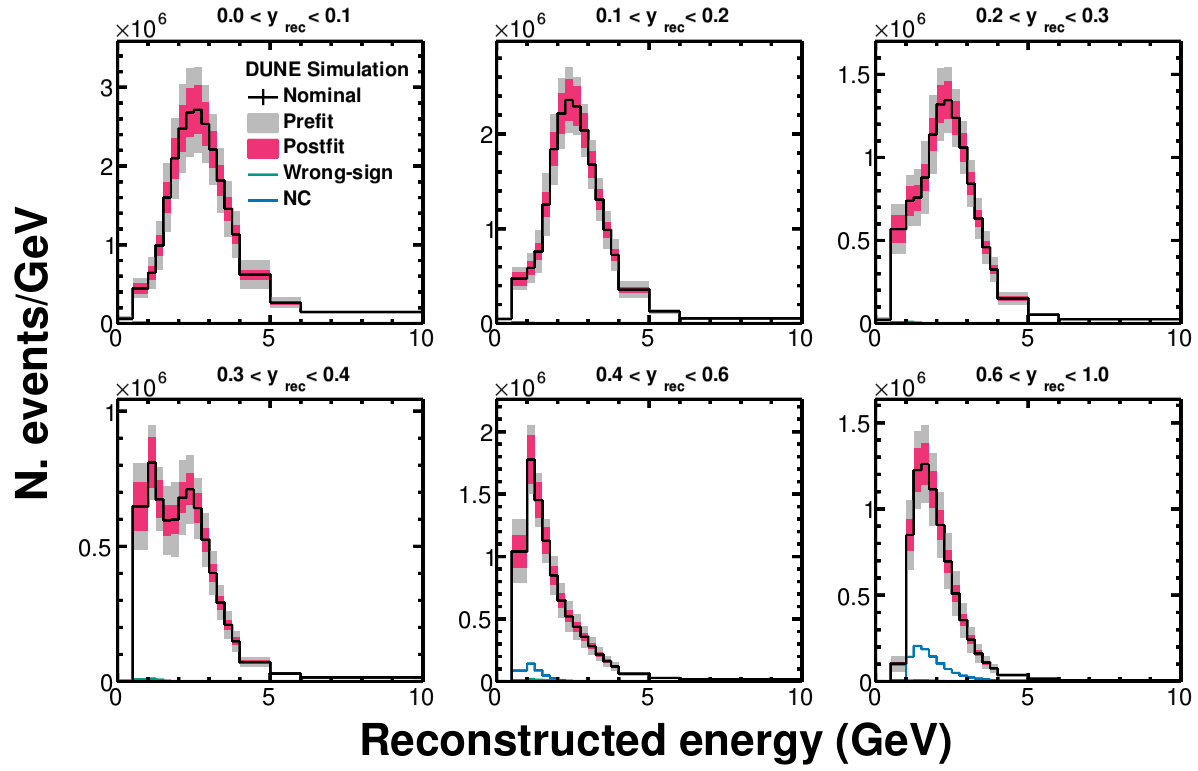
\includegraphics[width=0.8\linewidth]{ND_FHC_ndfd100ktMWyr_allsyst_asimov0_th13_constraint.png}}\\
  \subfloat[RHC]{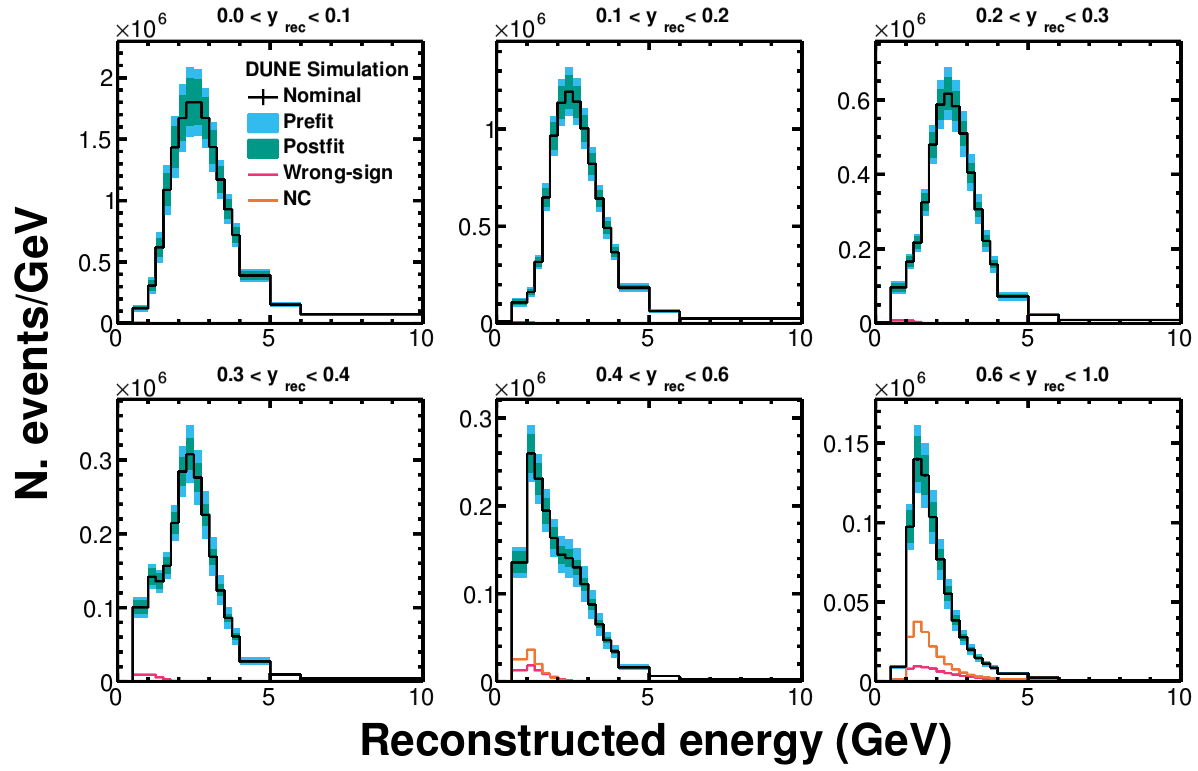
\includegraphics[width=0.8\linewidth]{ND_RHC_ndfd100ktMWyr_allsyst_asimov0_th13_constraint.png}}
  \caption{ND samples in both FHC and RHC, shown in the reconstructed neutrino energy and reconstructed inelasticity binning used in the analysis, shown for a $\sim$105 ton-year exposure (equivalent to a 100 ktMWyr exposure at the FD), with an equal split between FHC and RHC. The size of the systematic uncertainty bands from all of the flux, cross-section and ND detector systematics used in the analysis are shown, as well as the postfit uncertainty bands obtained by performing an Asimov fit to the ND data. Background are also shown, which are dominated by NC events, although there is some contribution from wrong-sign \numu background events in RHC.}
 \label{fig:nd_samples}
\end{figure*}
The oscillation analysis presented here includes samples of $\nu_{\mu}$ and $\bar{\nu}_{\mu}$ charged-current interactions originating in the LAr portion of the ND. These samples are binned in two dimensions as a function of reconstructed neutrino energy and inelasticity, $y_{\mathrm{rec}} = 1 - E^{\mathrm{rec}}_{\mu}/E^{\mathrm{rec}}_{\nu}$, where $E^{\mathrm{rec}}_{\mu}$ and $E^{\mathrm{rec}}_{\nu}$ are the reconstructed muon and neutrino energies, respectively. The sample distributions for both FHC and RHC are shown in Figure~\ref{fig:nd_samples} for an exposure of $\sim$105 ton-years, equivalent to 100 ktMWyr at the far detector with the assumptions stated above. The size of the systematic uncertainty bands from all of the flux, cross-section and ND detector systematics used in the analysis and described above are shown, as well as the postfit uncertainty bands obtained by performing an Asimov fit to the ND data. It is clear that even after a relatively small exposure of 105 ton-years, the ND samples are very high statistics, and are systematics limited in the binning used in the analysis. Backgrounds in the $\nu^{\bracketbar}_{\mu}$-CC samples are also shown in Figure~\ref{fig:nd_samples}: NC backgrounds are predominantly from NC $\pi^{\pm}$ production where the pion leaves a long track and does not shower; wrong-sign contamination in the beam is a background where the charge of the muon is not reconstructed, which particularly affects low reconstructed neutrino energies in RHC.

\begin{figure}[htbp]
 \subfloat[FHC]{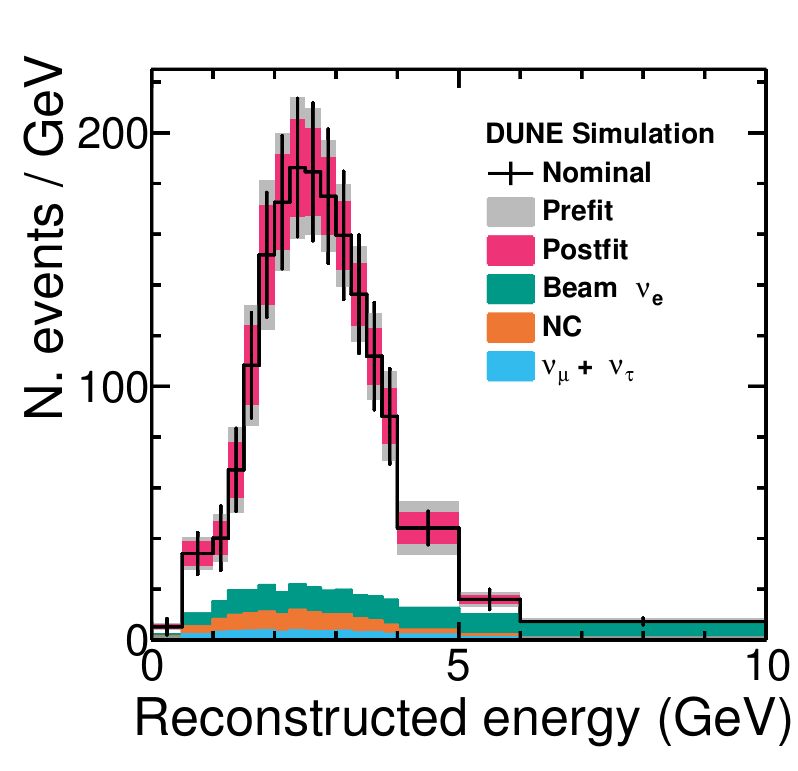
\includegraphics[width=0.8\linewidth]{FD_nue_FHC_ndfd100ktMWyr_allsyst_asimov0_th13_constraint.png}}\\
 \subfloat[RHC]{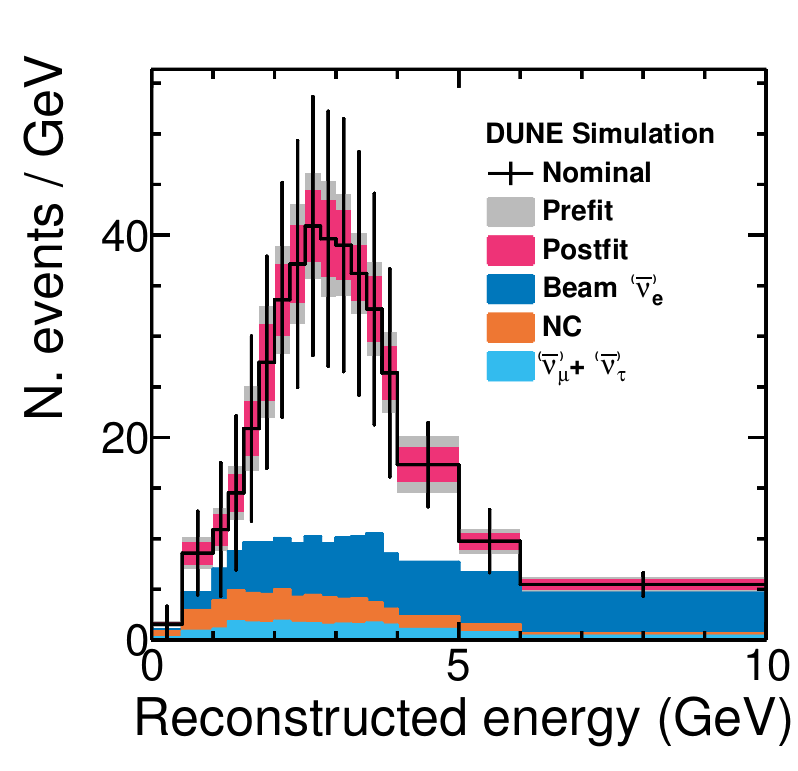
\includegraphics[width=0.8\linewidth]{FD_nue_RHC_ndfd100ktMWyr_allsyst_asimov0_th13_constraint.png}}
 \caption{Reconstructed energy distribution of selected CC $\nue^{\bracketbar}$-like events for a 50 ktMWyr exposure in both neutrino-enhanced FHC beam mode and antineutrino-enhanced RHC beam mode, for a total 100 ktMWyr year exposure. The plots are shown for NO, all other oscillation parameters are set to their NuFIT 4.0 best-fit values (see Table~\ref{tab:oscpar_nufit}). The size of the systematic uncertainty bands from all of the flux, cross-section and FD detector systematics used in the analysis are shown, as well as the postfit uncertainty bands with parameters constrained by ND data. Backgrounds are also shown, the largest contribution comes from intrinsic $\nue^{\bracketbar}$ contamination in the beam, although NC and other flavors, $\numu^{\bracketbar} + \nutau^{\bracketbar}$, also contribute.}
 \label{fig:appspectra}
\end{figure}
The expected FD FHC \nue and RHC \anue samples are shown in Figure~\ref{fig:appspectra} for a 100 ktMWyr total FD exposure, split equally into FHC and RHC beam modes. The systematic uncertainty bands with and without the ND constraint applied are shown, as well as the background contributions. Note that there are contributions from both \nue and \anue in both beam modes. The NC, intrinsic beam $\nue^{\bracketbar}$, and wrong flavor contamination is also shown, the largest background comes from the intrinsic $\nue^{bracketbar}$ beam contribution in both modes. After a 50 ktMWyr exposure in FHC, the \nue sample statistical uncertainty is close to the systematic uncertainty before the ND constraint, although is still clearly statistics limited when the ND constraint is applied. The \anue sample is still strongly statistics limited after 50 ktMWyr exposure in RHC. The difference is largely due to the difference in the \nue and \anue cross sections. The $\nue^{\bracketbar}$ samples in both modes are clearly statistics limited until much larger exposures.

\begin{figure}[htbp]
  \subfloat[FHC]{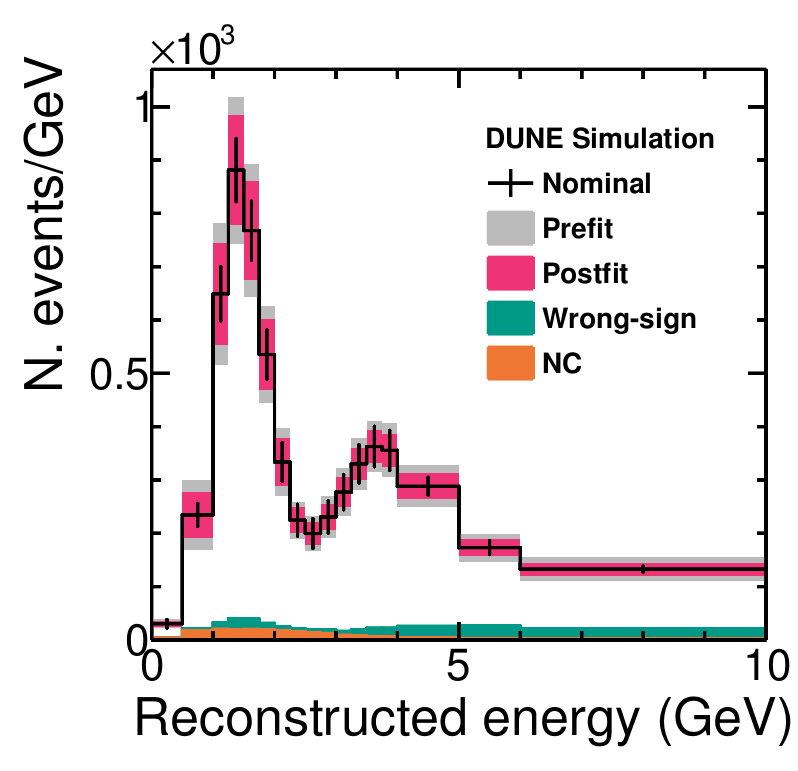
\includegraphics[width=0.8\linewidth]{FD_numu_FHC_ndfd100ktMWyr_allsyst_asimov0_th13_constraint.png}}\\
  \subfloat[RHC]{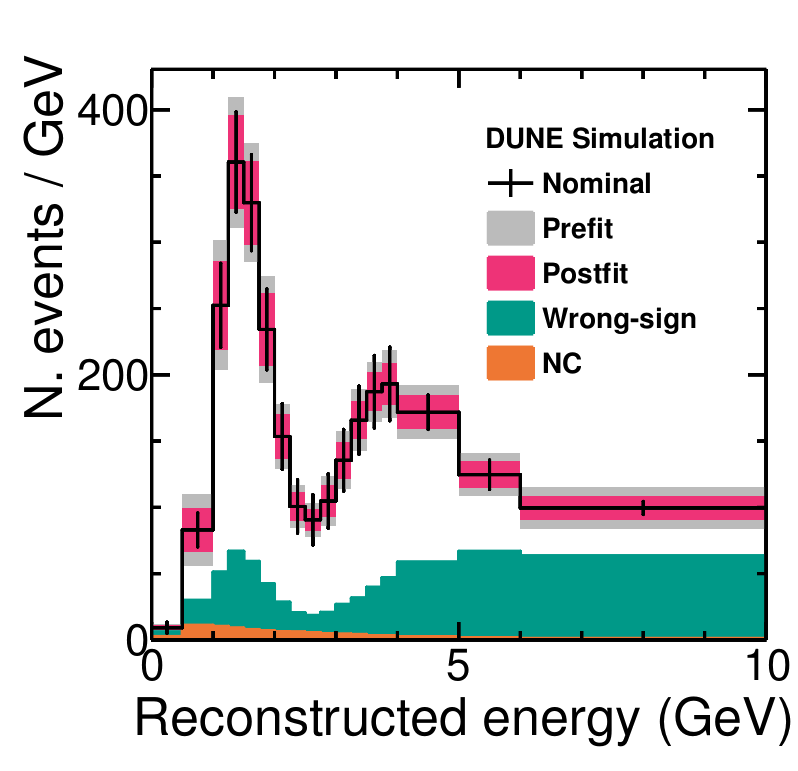
\includegraphics[width=0.8\linewidth]{FD_numu_RHC_ndfd100ktMWyr_allsyst_asimov0_th13_constraint.png}}
\caption{Reconstructed energy distribution of selected CC $\nu^{\bracketbar}_{\mu}$-like events for 50 ktMWyr exposure in both neutrino-enhanced FHC beam mode and antineutrino-enhanced RHC beam mode, for a total 100 ktMWyr year exposure. The plots are shown for NO, all other oscillation parameters are set to their NuFIT 4.0 best-fit values (see Table~\ref{tab:oscpar_nufit}). The size of the systematic uncertainty bands from all of the flux, cross-section and ND detector systematics used in the analysis are shown, as well as the postfit uncertainty bands with parameters constrained by ND data. NC and wrong-sign backgrounds are also shown, the only sizeable background is the wrong-sign (\numu) contribution to the RHC same.}
\label{fig:disspectra}
\end{figure}
The expected FD FHC \numu and RHC \anumu samples are shown in Figure~\ref{fig:disspectra} for a 100 ktMWyr total FD exposure, split equally into FHC and RHC beam modes. The systematic uncertainty bands with and without the ND constraint applied are shown, as well as the background contributions. Note that although the wrong-sign \numu contribution to the RHC \anumu sample is identified as a background, it still provides useful information, it just complicates the analysis. The statistics are much higher than in Figure~\ref{fig:appspectra}, the statistical uncertainty on the \numu FHC sample is smaller than the systematic uncertainty band for some regions of phase space, even after the ND constraint is applied, although the statistical uncertainty is larger than the constrained systematic uncertainty in the ``dip'' region, around 2.5 GeV, which is likely to have the most impact on the analysis. The statistical uncertainty on the \anumu RHC sample is larger, again due to the smaller \anumu than \numu cross section, and the statistical uncertainty around the 2.5 GeV dip region is significantly larger than the systematic uncertainty band, although as for the FHC \numu sample, the statistical uncertainty is smaller than the systematics for some regions of the parameter space.

Note that the events with reconstructed neutrino energy less than 0.5 GeV (which are shown in Figures~\ref{fig:appspectra} and~\ref{fig:disspectra}) or neutrino energies greater than 10 GeV are not included in the analysis for any of the FD or ND samples.




\section{Run plan optimization}
\label{sec:run_plan_opt}
In previous DUNE sensitivity studies~\cite{Abi:2020qib}, equal running times in FHC and RHC were assumed, based on early sensitivity estimates for different scenarios. In this section, the dependence of the median CPV and mass ordering significances are studied, for different fractions of time spent in each beam mode, using the full analysis framework described in Section~\ref{sec:analysis_framework}.
\begin{figure*}[htbp]
  \centering
  \subfloat[NO, with $\theta_{13}$-penalty] {\includegraphics[width=0.4\linewidth]{{cpv_sens_ndfd100kTMWyr_th13_asimov0_nh}.png}}
  \subfloat[IO, with $\theta_{13}$-penalty] {\includegraphics[width=0.4\linewidth]{{cpv_sens_ndfd100kTMWyr_th13_asimov0_ih}.png}}\\
  \subfloat[NO, no $\theta_{13}$-penalty]   {\includegraphics[width=0.4\linewidth]{{cpv_sens_ndfd100kTMWyr_nopen_asimov0_nh}.png}}
  \subfloat[IO, no $\theta_{13}$-penalty]   {\includegraphics[width=0.4\linewidth]{{cpv_sens_ndfd100kTMWyr_nopen_asimov0_ih}.png}}
  \caption{The Asimov CPV sensitivity as a function of the true value of \deltacp, for a total exposure of 100 kt-MW-yrs with different fractions of FHC and RHC running, with and without a $\theta_{13}$ penalty applied in the fit. Results are shown for both true normal and inverted ordering, with the true oscillation parameter values set to the NuFit 4.0 best fit point in each ordering (see Table~\ref{tab:oscpar_nufit}).}
  \label{fig:run_opt_cpv}
\end{figure*}

Figure~\ref{fig:run_opt_cpv} shows DUNE's Asimov sensitivity to CPV for a total 100 kt-MW-yrs far detector exposure, with different fractions of FHC and RHC running, at the NuFIT 4.0 best fit value in both NO and IO (see Table~\ref{tab:oscpar_nufit}), shown with and without a penalty on $\theta_{13}$ applied. For each point tested, all oscillation and nuisance parameters are allowed to vary, and two fits are carried out, one where \deltacp is only allowed to take CP-conserving values, and another where it is allowed to vary. The difference in the best-fit $\chi^{2}$ values is calculated:
\begin{equation}
  \Delta\chi^{2} = \min\left\{\chi^{2}_{\deltacp = -\pi},\chi^{2}_{\deltacp = 0},\chi^{2}_{\deltacp = \pi}\right\} - \chi^{2}_{\mathrm{CPV}},
  \label{eq:cpv_chi2}
\end{equation}
\noindent and the square root of the difference is  used as the figure of merit on the y-axis in Figure~\ref{fig:run_opt_mh}. We note that there are some caveats associated with this figure of merit, which are discussed in Section~\ref{sec:cp_sens}. A 100 kt-MW-yrs exposure is shown as it was identified in Ref~\cite{Abi:2020qib} as the exposure at which DUNE's median CPV significance exceeds 3$\sigma$ at $\deltacp = \pm\pi/2$, an important milestone in DUNE's physics program (with equal beam mode running). 

%\chris{I find this paragraph jargony, i.e. terms like ``th13 penalty'' and ``octant degeneracy'' could be explained a bit more.  I have attempted a rewrite below.}
%Figure~\ref{fig:run_opt_cpv} shows that with a $\theta_{13}$ applied, the sensitivity to CPV can be increased in some regions of \deltacp parameter space with more FHC than RHC running. However this degrades the sensitivity in other regions, most notably for $\deltacp > 0$ regardless of the true mass ordering, where the octant degeneracy starts to strongly impact the results. For regions of phase space where the octant degeneracy does not affect the result (e.g., $\sin^{2}\theta_{23} \approx 0.5$), there is no degredation in the sensitivity, and enhanced FHC running increases the sensitivity for all values of \deltacp. Increasing the fraction of RHC decreases the sensitivity for the entire \deltacp range when the $\theta_{13}$ penalty is applied, relative to equal beam mode running, which can be understood as being due to the lower statistics of the \anue sample (see Figure~\ref{fig:appspectra}). Although for low exposures, DUNE will not have a strong constraint on $\theta_{13}$, so the main analysis will include a $\theta_{13}$ penalty, it is instructive to look at the results without the penalty applied. In the no penalty case, the sensitivity is severely degraded (as expected) for 100\% running in either beam mode.

Figure~\ref{fig:run_opt_cpv} shows that when the reactor constraint on $\theta_{13}$ is included, the sensitivity to CPV can be increased in some regions of \deltacp parameter space with more FHC than RHC running. However, this degrades the sensitivity in other regions, most notably for $\deltacp > 0$ regardless of the true mass ordering. This is due to a degeneracy between \deltacp and the octant of $\sinstt{23}$ because both parameters impact the rate of \nue appearance. The degeneracy is resolved by including antineutrino data; the octant of $\sinstt{23}$ affects the rate of \nue and \anue appearance in the same way, but the effect of \deltacp is reversed for antineutrinos.

For regions of phase space where the octant degeneracy does not affect the result (e.g., $\sin^{2}\theta_{23} \approx 0.5$), there is no degredation in the sensitivity, and enhanced FHC running increases the sensitivity for all values of \deltacp. Increasing the fraction of RHC decreases the sensitivity for the entire \deltacp range when the reactor $\theta_{13}$ constraint is included, relative to equal beam mode running. This is due to the lower statistics of the \anue sample (see Figure~\ref{fig:appspectra}) because of the reduced antineutrino flux and cross section. For short exposures, DUNE will not have a competitive independent measurement of $\theta_{13}$, so the main analysis will include the reactor $\theta_{13}$ constraint. Nonetheless, it is instructive to look at the results without the penalty applied. In this case, the sensitivity is severely degraded (as expected) for 100\% running in either beam mode.


\begin{figure*}[htbp]
  \centering
  \subfloat[NO, with $\theta_{13}$-penalty]  {\includegraphics[width=0.4\linewidth]{{mh_sens_ndfd24kTMWyr_th13_asimov0_nh}.png}}
  \subfloat[IO, with $\theta_{13}$-penalty]  {\includegraphics[width=0.4\linewidth]{{mh_sens_ndfd24kTMWyr_th13_asimov0_ih}.png}}\\
  \subfloat[NO, no $\theta_{13}$-penalty]    {\includegraphics[width=0.4\linewidth]{{mh_sens_ndfd24kTMWyr_nopen_asimov0_nh}.png}}
  \subfloat[IO, no $\theta_{13}$-penalty]    {\includegraphics[width=0.4\linewidth]{{mh_sens_ndfd24kTMWyr_nopen_asimov0_ih}.png}}
  \caption{The Asimov mass ordering sensitivity as a function of the true value of \deltacp, for a total exposure of 24 kt-MW-yrs with different fractions of FHC and RHC running, with and without a $\theta_{13}$ penalty applied in the fit. Results are shown for both true normal and inverted ordering, with the true oscillation parameter values set to the NuFIT 4.0 best fit point in each ordering (see Table~\ref{tab:oscpar_nufit}).}
  \label{fig:run_opt_mh}
\end{figure*}
Figure~\ref{fig:run_opt_mh} shows DUNE's Asimov sensitivity to the mass ordering for a total 24 kt-MW-yrs far detector exposure, with different fractions of FHC and RHC running, and the same four true oscillation parameter sets. For each point tested, all oscillation and nuisance parameters are allowed to vary, and two fits are carried out, one using each ordering. The difference in the best-fit $\chi^{2}$ values is calculated:
\begin{equation}
  \Delta\chi^{2} = \chi^{2}_{\mathrm{IO}} - \chi^{2}_{\mathrm{NO}},
  \label{eq:mh_chi2}
\end{equation}
\noindent and the square root of the difference is used as the figure of merit on the y-axis in Figure~\ref{fig:run_opt_mh}. We note that there are some caveats associated with this figure of merit, which are discussed in Section~\ref{sec:mh_sens}. A 24 kt-MW-yrs exposure is used in Figure~\ref{fig:run_opt_mh} as it is around the exposure at which DUNE's median mass ordering significance exceeds 5$\sigma$ for some vales of \deltacp~\cite{Abi:2020qib}.

It is clear from Figure~\ref{fig:run_opt_mh} that the mass ordering sensitivity has a strong dependence on the fraction of running in each beam mode. As in the CPV case, the effect is very different with and without the reactor $\theta_{13}$ constraint included. If the true ordering is normal and the reactor $\theta_{13}$ penalty is applied, the sensitivity increases significantly with increasing FHC running, with a full 1$\sigma$ increase in the sensitivity between equal beam running and 100\% FHC for most values of \deltacp. Conversely, if the ordering is inverted, 100\% FHC running would degrade the sensitivity by $\geq$1$\sigma$ for all values of \deltacp at the NuFIT 4.0 best fit point. Overall the sensitivity to the inverted ordering is improved by a more equal split between the beam modes. It is clear that 100\% RHC running gives poor sensitivity for all values tested. 

Without the reactor $\theta_{13}$ constraint, the greatest sensitivity is obtained with close to an equal split of FHC and RHC running, and the sensitivity is significantly reduced with 100\% FHC running. This is because of a degeneracy between the effect of $\theta_{13}$ and the mass ordering on the rate of \nue appearance in FHC mode. If the mass ordering is normal, the \nue rate in FHC will be enhanced; without the reactor constraint, this excess can be accommodated by increasing the value of $\theta_{13}$.

\begin{figure*}[htbp]
  \centering
  \subfloat[CPV, with $\theta_{13}$-penalty] {\includegraphics[width=0.4\linewidth]{{cpv_sens_ndfd334kTMWyr_th13_asimov0_nh}.png}}
  \subfloat[CPV, no $\theta_{13}$-penalty]   {\includegraphics[width=0.4\linewidth]{{cpv_sens_ndfd334kTMWyr_nopen_asimov0_nh}.png}}\\
  \subfloat[MO, with $\theta_{13}$-penalty]  {\includegraphics[width=0.4\linewidth]{{mh_sens_ndfd334kTMWyr_th13_asimov0_nh}.png}}
  \subfloat[MO, no $\theta_{13}$-penalty]    {\includegraphics[width=0.4\linewidth]{{mh_sens_ndfd334kTMWyr_nopen_asimov0_nh}.png}}
  \caption{The Asimov CPV and mass ordering sensitivities as a function of the true value of \deltacp, for a total exposure of 334 kt-MW-yrs with different fractions of FHC and RHC running, with and without a $\theta_{13}$ penalty applied in the fit. Results are shown for both true normal ordering only, with the true oscillation parameter values set to the NuFIT 4.0 NO best fit point (see Table~\ref{tab:oscpar_nufit}).}
  \label{fig:run_opt_334ktmwyr}
\end{figure*}

For comparison, Figure~\ref{fig:run_opt_334ktmwyr} shows the Asimov CPV and mass ordering sensitivities, with and without the reactor $\theta_{13}$ constraint included, for true normal ordering only, for a large exposure of 334 kt-MW-yrs, with different fractions of FHC and RHC running. At large exposures, running with strongly enhanced FHC running no longer improves the sensitivity over equal beam mode running, with or without the $\theta_{13}$ penalty applied, for either CPV or mass ordering determination. 

Overall, the sensitivity to CPV and the mass ordering is dependent on the division of running time between FHC and RHC, but a choice that increases the sensitivity in some region of parameter space can severely decrease the sensitivity in other regions. If there is strong reason to favor, for example, normal over inverted ordering when DUNE starts to take data, Figure~\ref{fig:run_opt_mh} shows that this could be more rapidly verified by running with more FHC data than RHC data, as the reactor $\theta_{13}$ constraint will be used in the main low exposure analysis. However, if this choice is wrong, this might cause DUNE to take longer to reach the same significance. Clearly this is an important consideration which should be revisited shortly before DUNE begins to collect data. Similarly, the CPV sensitivity shown in Figure~\ref{fig:run_opt_cpv} might be optimized if there is a strong reason to favor gaining sensitivity for $\deltacp > 0$ or $\deltacp < 0$, at a cost of reducing the sensitivity to CPV if \deltacp has the other sign. But, it is clear from Figures~\ref{fig:run_opt_cpv} and~\ref{fig:run_opt_mh} that equal running in FHC and RHC gives a close to optimal sensitivity across all of the parameter space, and as such is a reasonable {\it a priori} choice of run plan for studies of the DUNE sensitivity. Additionally, it is clear from Figure~\ref{fig:run_opt_334ktmwyr} that the improvement in the sensitivity with unequal beam running is a feature at low exposures, but not at high exposures, particularly because at high exposures when DUNE is able to constrain all the oscillation parameters with precision~\cite{Abi:2020qib}, there is a stronger motivation to run a DUNE-only analysis, without relying on the reactor $\theta_{13}$ measurement.



\FloatBarrier
\section{CP violation sensitivity}
\label{sec:cp_sens}

In this section, CPV sensitivity results are presented. For simplicity, only true NO will be shown unless explicitly stated. In all cases, a joint ND+FD fit is performed, and a $\theta_{13}$ penalty is always applied, as described in Section~\ref{sec:analysis_framework}. An equal split between FHC and RHC running is assumed based on the results obtained in Section~\ref{sec:run_plan_opt}. The Asimov sensitivities as shown in Section~\ref{sec:run_plan_opt} are informative, but do not give information on how the expected sensitivity may vary with statistical or systematic uncertainties. Or for variations in the other oscillation parameters of interest.

\begin{figure}[htbp]
  \centering
  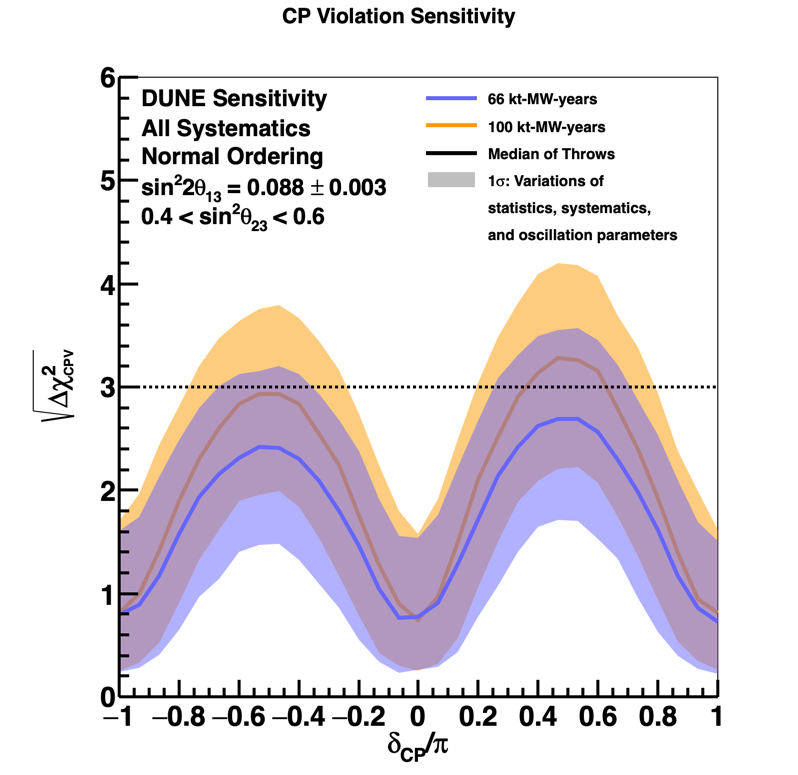
\includegraphics[width=0.8\linewidth, trim={0cm 0cm 0cm 2.3cm}, clip]{cpv_two_exps_throws_nh_2019_v4_lowexp.png}\\
  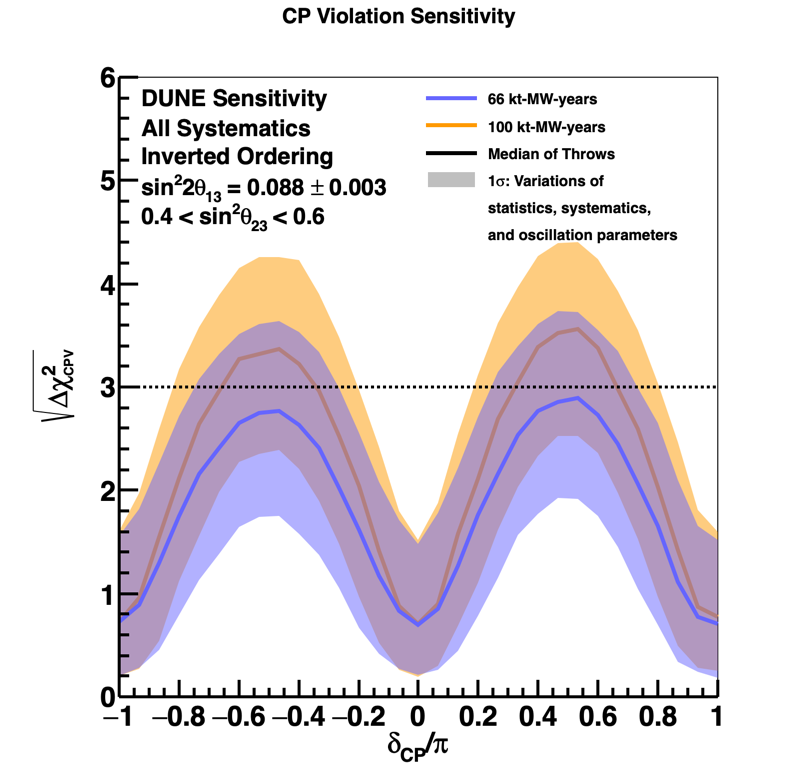
\includegraphics[width=0.8\linewidth, trim={0cm 0cm 0cm 2.3cm}, clip]{cpv_two_exps_throws_ih_2019_v4_lowexp.png}
  \caption{Significance of the DUNE determination of CP-violation ($\deltacp \neq [0,\pm\pi]$) as a function of the true value of \deltacp, for 66 ktMWyr (blue) and 100 ktMWyr (orange) exposures, for normal (top) and inverted (bottom) orderings. The width of the transparent bands cover 68\% of fits in which random throws are used to simulate systematic, oscillation parameter and statistical variations, with independent fits performed for each throw constrained by pre-fit uncertainties. The solid lines show the median sensitivity.}
  \label{fig:cpv_bands}
\end{figure}
Figure~\ref{fig:cpv_bands} shows the significance with which CPV ($\deltacp \neq [0, \pm\pi]$) can be observed for both NO and IO, for exposures of 66 kTMWyr and 100 ktMWyr. For each throw of the systematic, other oscillation parameters and statistics, two fits are carried out, one where the \deltacp is fixed at CP-conserving values, and another where it is allowed to vary. The difference in the best-fit $\chi^{2}$ values is calculated:
\begin{equation}
  \Delta\chi^{2} = \chi^{2}_{0,\pm\pi} - \chi^{2}_{\mathrm{CPV}},
  \label{eq:cpv_chi2}
\end{equation}
\noindent and the square root of the difference is the significance shown on the y-axis of Figure~\ref{fig:cpv_bands}. We note that this constant-\dchisq method is valid as long as Wilks' can be applied~\cite{wilks}.

The sensitivity shown in Figure~\ref{fig:cpv_bands} has the characteristic double peak structure because the significance of a CPV measurement decreases around CP-conserving values. The median sensitivity never reaches exactly zero at CP-conserving values due to the systematic and statistical throws. Median sensitivities are slightly higher for IO than for NO, and by exposures of 100 ktMWyr, the median sensitivity exceeds 3$\sigma$ for the maximal CP-violating values of $\pm\pi/2$. This presentation of the CPV sensitivity was followed in Ref.~\cite{Abi:2020qib}, and is very informative at high exposures. However at low exposures as shown in Figure~\ref{fig:cpv_bands}, the spread in the sensitivity is harder to interpret.

\begin{figure*}[htbp]
  \centering
  \subfloat[24 ktMWyr] {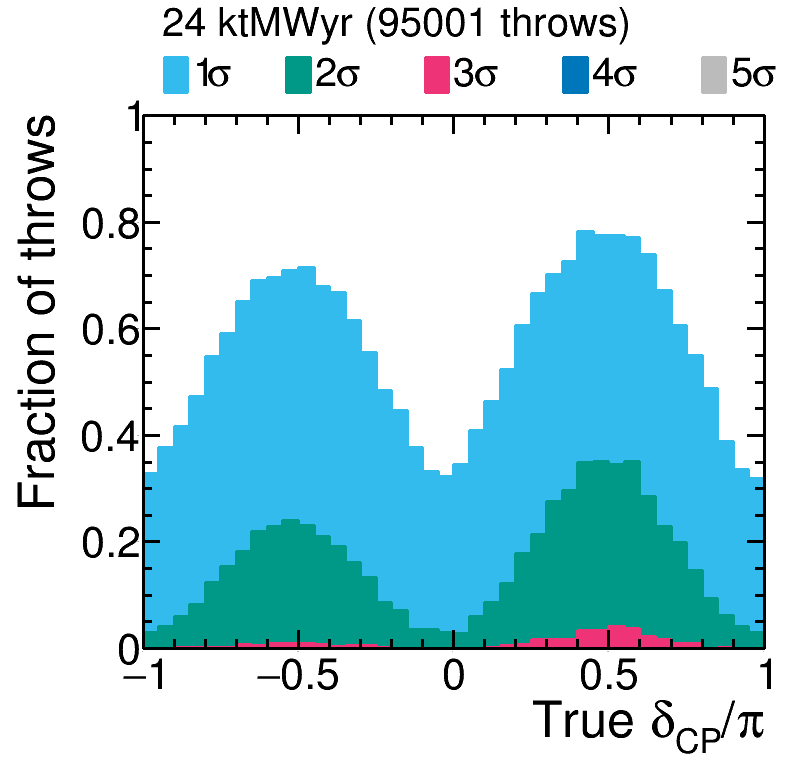
\includegraphics[width=0.33\linewidth]{cpv_throws_24ktMWyr_NH_th13.png}}
  \subfloat[66 ktMWyr] {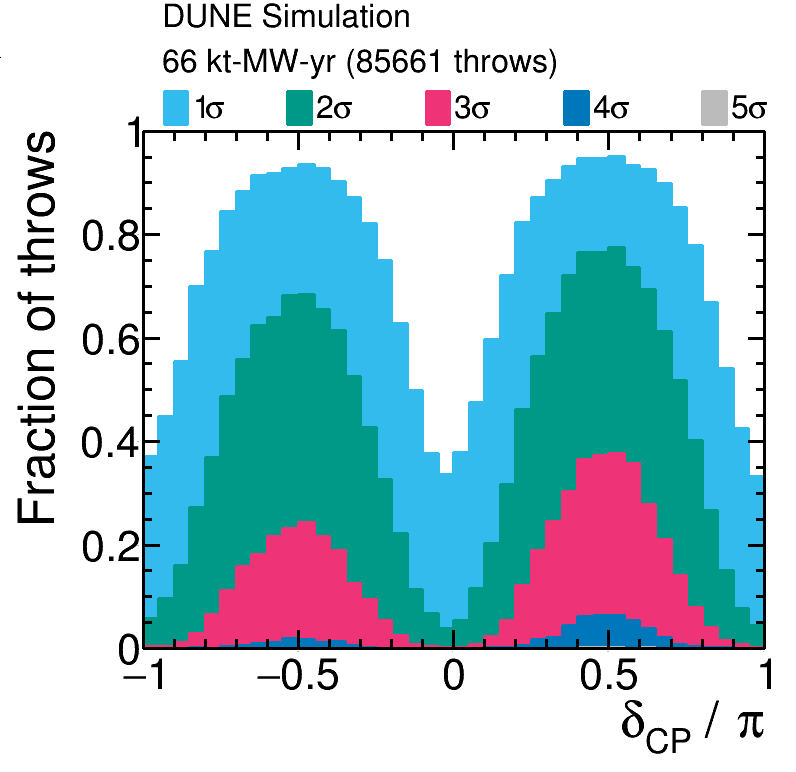
\includegraphics[width=0.33\linewidth]{cpv_throws_66ktMWyr_NH_th13.png}}
  \subfloat[100 ktMWyr]{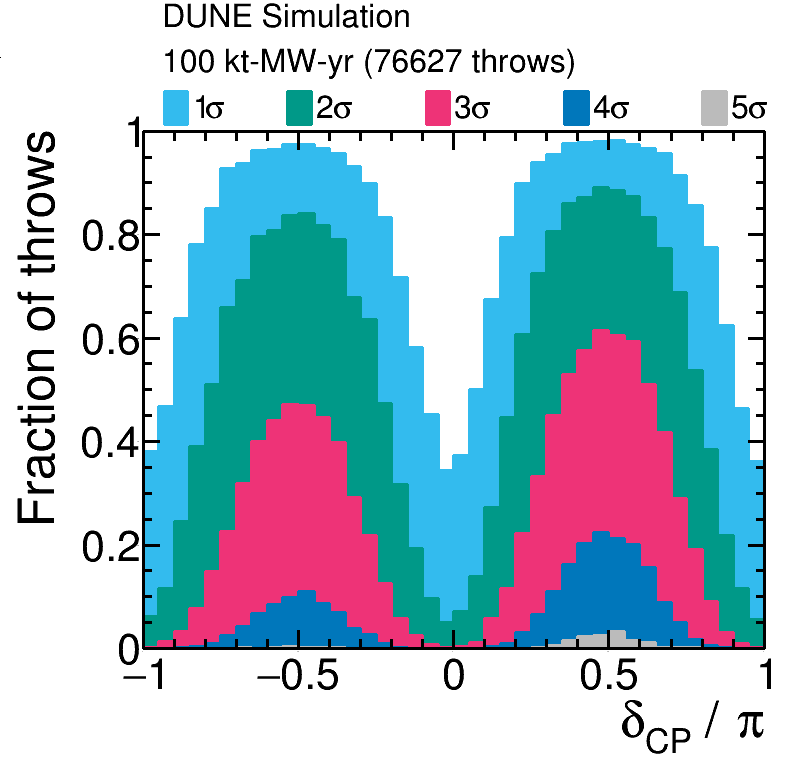
\includegraphics[width=0.33\linewidth]{cpv_throws_100ktMWyr_NH_th13.png}}\\
  \subfloat[150 ktMWyr]{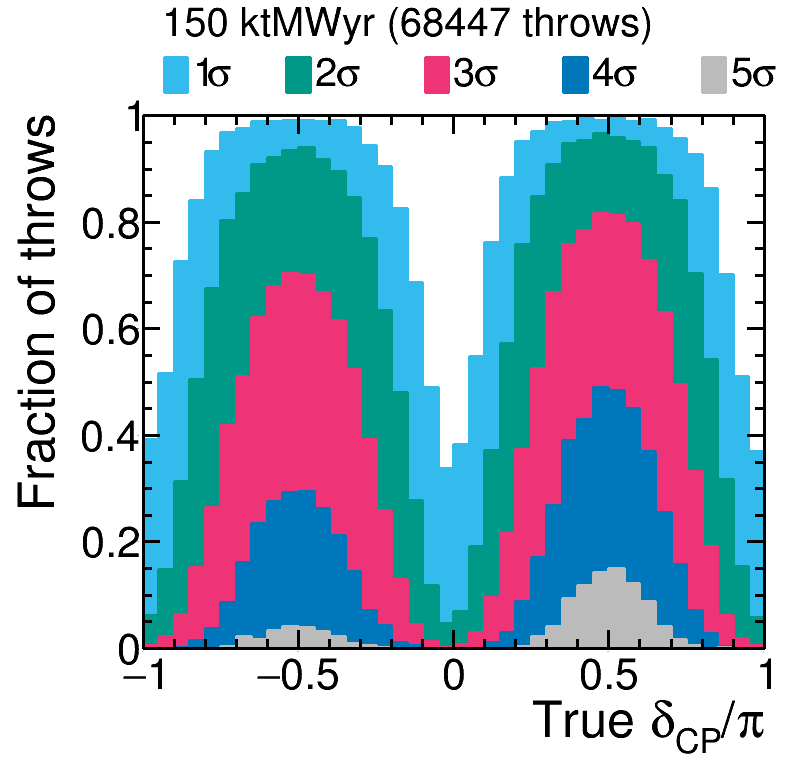
\includegraphics[width=0.33\linewidth]{cpv_throws_150ktMWyr_NH_th13.png}}
  \subfloat[197 ktMWyr]{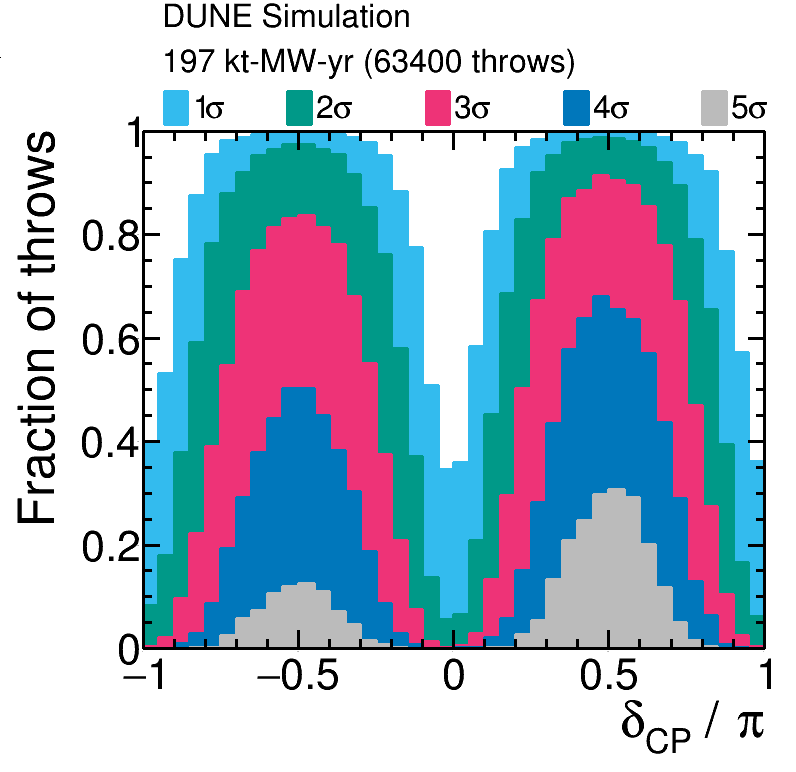
\includegraphics[width=0.33\linewidth]{cpv_throws_197ktMWyr_NH_th13.png}}
  \subfloat[334 ktMWyr]{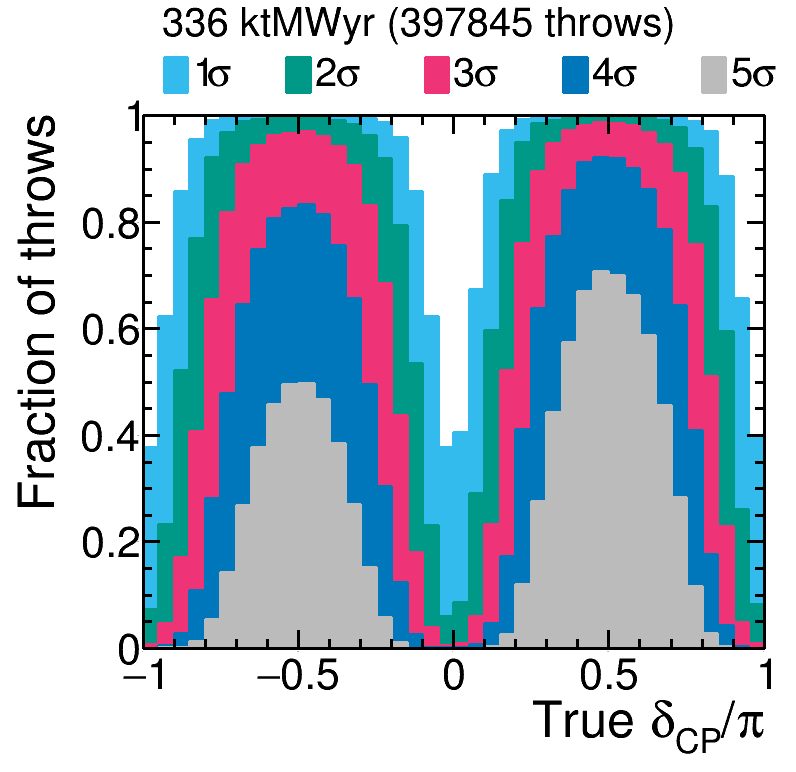
\includegraphics[width=0.33\linewidth]{cpv_throws_334ktMWyr_NH_th13.png}}
  \caption{Fraction of throws for which the DUNE sensitivity to CP-violation ($\deltacp \neq [0,\pm\pi]$) exceeds 1--5$\sigma$ significance, as a function of the true value of \deltacp. Shown for NO, for a number of different exposures. The number of throws used to make each figure is also shown.}
  \label{fig:cpv_over_time}
\end{figure*}
\begin{figure*}[htbp]
  \centering
  \subfloat[$\deltacp = -\pi/2$] {\includegraphics[width=0.8\columnwidth]{{fraction_throws_vs_exp_dcp-0.5}.pdf}}
  \subfloat[$\deltacp = +\pi/2$] {\includegraphics[width=0.8\columnwidth]{{fraction_throws_vs_exp_dcp0.5}.pdf}}
  \caption{Fraction of throws for which the DUNE sensitivity to CP-violation ($\deltacp \neq [0,\pm\pi]$) exceeds 1--5$\sigma$ significance, at $\deltacp = \pm\pi/2$, shown as a function of exposure, for NO.}
  \label{fig:cpv_vs_exp}
\end{figure*}
Figure~\ref{fig:cpv_over_time} provides an alternative way to present the results of the throws. The fraction of throws for which Equation~\ref{eq:cpv_chi2} exceeds different confidence values are shown, for 1--5$\sigma$ significances, for a variety of exposures. It shows the probability for DUNE to observe a significance above a discrete threshold, as a function of the true value of \deltacp. The point at which the median sensitivity (50\% of throws) passes different significance thresholds can be easily read from the figures, and can be compared with those shown in Figure~\ref{fig:cpv_bands}. Note that the highest exposure shown, 334 ktMWyr, is equivalent to the seven year exposure using the staging scenario from Ref.~\cite{Abi:2020qib}. The same double peak structure seen in Figure~\ref{fig:cpv_bands} can be observed. The median sensitivity to CPV exceeds 3$\sigma$ after $\sim$100 ktMWyr, but a significant fraction of throws exceed 3$\sigma$ at 66 ktMWyr. Likewise, although the median significance to CPV does not exceed 5$\sigma$ until $\sim$334 ktMWyr, there are significant fractions of throws at lower exposures which reach $5\sigma$ significance. This presentation also shows that by 334 ktMWyr exposures, the number of throws for which the significance is less than 3$\sigma$ at maximal values of \deltacp is very low. The number of throws used to generate the plots at each exposure is indicated on each plot. The number of throws decreases as a function of exposure because fixed computing resources were used for each configuration, and the time for the ensemble of fits carried out for each throw to complete increases slightly with exposure. The final 334 ktMWyr exposure has more throws because it was generated for the analysis presented in Ref.~\cite{Abi:2020qib}, where more than one projection was considered --- requiring more throws to sample the space.

Figure~\ref{fig:cpv_vs_exp} shows the fraction of throws which exceed different significance thresholds at the maximal \deltacp violation values of $\pm\pi/2$, as a function of exposure. Figure~\ref{fig:cpv_vs_exp} was produced using the same throws used for Figure~\ref{fig:cpv_over_time}, with additional points from higher exposures used in Ref.~\cite{Abi:2020qib}, but not shown in Figure~\ref{fig:cpv_over_time} (646 ktMWyr and 1104 ktMWyr). For NO, the significance at $\deltacp = +\pi/2$ is slightly stronger than at $\deltacp = -\pi/2$. For IO, the significance would be more similar between the two points, which can be observed from Figure~\ref{fig:cpv_bands}, but is not shown in Figures~\ref{fig:cpv_over_time} or~\ref{fig:cpv_vs_exp}.

% \FloatBarrier
% \subsection{Feldman-Cousins studies}
Previous results have been calculated confidence intervals and significances using constant $\Delta\chi^{2}$ critical values. For example, in the CPV results shown in Figure~\ref{fig:cpv_over_time}, the confidence intervals are calculated assuming one degree of freedom, so $\Delta\chi^{2} \leq 1, 4, 9$ corresponds to a significance of 1, 2 and 3$\sigma$. This assumption holds when Wilks' theorem can be applied~\cite{wilks}, but can lead to incorrect coverage where it cannot. This breaks down around physical boundaries, in the case of cyclic parameters, and where there are significant degeneracies. It is likely that a constant $\Delta\chi^{2}$ treatment will break down for \deltacp, where all of these issues apply, as has indeed been shown by T2K~\cite{Abe:2021gky}. The Feldman-Cousins method~\cite{Feldman:1997qc} is a brute force numerical method to calculate confidence intervals with correct coverage.

A large number of toy experiments are produced, where the parameter(s) of interest (here \deltacp) is set to the desired true value, all other systematic and oscillation parameters are thrown, as described in Section~\ref{sec:analysis_framework}, and a statistical throw is made, for the two ND samples and four FD sample used in the analysis. Then two fits are performed, one where the parameter(s) of interest is fixed to the true value, and another where is is allowed to vary. In both fits, all other parameters are allowed to vary. For each throw, a \dchisq is calculated using the minimum $\chi^{2}$ values for those two fits, as in Equation~\ref{dchisq_fc}.
\begin{equation}
  \Delta\chi^{2} = \chi^{2}(\theta_{\mathrm{true}}) - \min_{\theta}\chi^{2}(\theta)
  \label{eq:dchisq_fc}
\end{equation}
\begin{figure}[htbp]
  \centering
  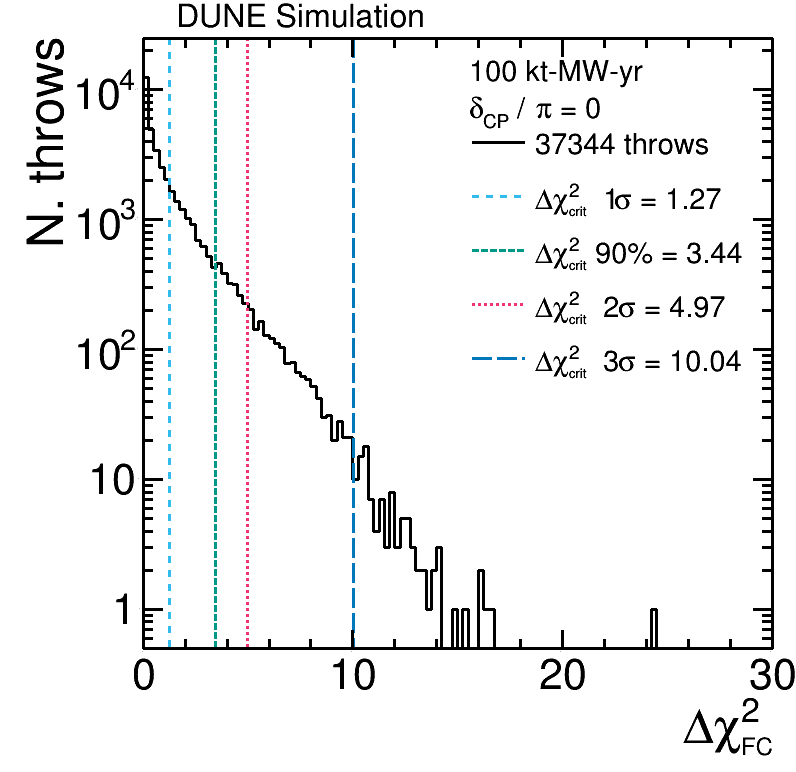
\includegraphics[width=0.8\columnwidth]{nh_FC_ndfd_100ktMWyr_dcp0.png}
  \caption{Distribution of \dchisq values, calculated using Equation~\ref{eq:dchisq_fc}, for a large number of throws with true $\deltacp = 0$, and a 100 ktMWyr exposure. The \dchisqcrit values (vertical lines) obtained using the Feldman-Cousins method show the \dchisq value below which 68.27\% (1$\sigma$), 90\%, 95.45\% (2$\sigma$) and 99.73\% (3$\sigma$) of throws reside, with the calculated values given in the legend. The number of throws used is also given.}
  \label{fig:fc_throws}
\end{figure}
The distribution of these throws is used to calculate the \dchisqcrit that gives the desired coverage, with the appropriate fraction of toys above/below the calculated value. A distribution of \dchisq values is shown in Figure~\ref{fig:fc_throws} for an example ND+FD analysis with a 100ktMWyr exposure at the far detector, equal FHC and RHC run fractions, and with a $\theta_{13}$ penalty applied. In Figure~\ref{fig:fc_throws}, the \dchisqcrit values corresponding to for 68.27\% (1$\sigma$), 90\%, 95.45\% (2$\sigma$) and 99.73\% (3$\sigma$) of the throws are indicated. The \dchisqcrit values were only calculated up to the 3$\sigma$ level due to the very large number of throws required for higher confidence levels.

An uncertainty on the value of \dchisqcrit obtained from the toy throw distribution (e.g., Figure~\ref{fig:fc_throws}), is obtained using a bootstrap rethrowing method~\cite{rice2006mathematical}. The empirical PDF obtained from the throws is treated as the true PDF, and $B$ independent samples of size $n$ are drawn from it, where $n$ is the total number of throws used to build the empirical PDF. Note that each throw can be drawn multiple times in this method. Then, the standard deviation $s_{\hat{\vartheta}}$, on the \dchisqcrit values of interest, $\vartheta$, are calculated for each of the $B$ samples using:
\begin{equation}
  s_{\hat{\vartheta}} = \sqrt{\frac{1}{B} \sum^{B}_{i=0} (\vartheta_{i}^{*} - \bar{\vartheta}^{*})^{2}},
  \label{eq:fc_uncertainty}
\end{equation}
where $\vartheta_{i}^{*}$ denotes the calculated \dchisqcrit value of interest for each of the samples, and $\bar{\vartheta}^{*}$ is their average value.

\begin{figure}[htbp]
  \centering
  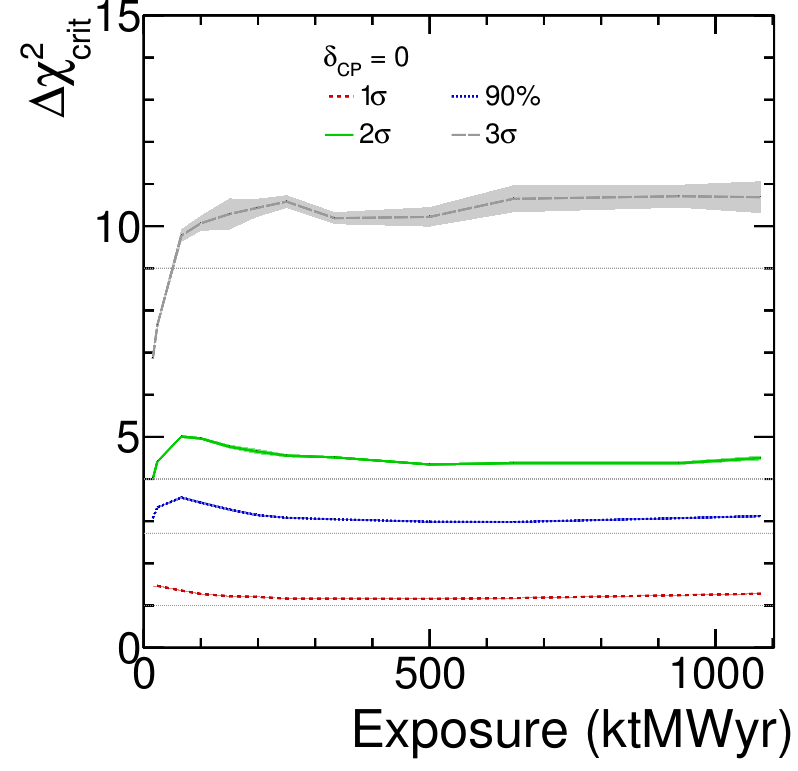
\includegraphics[width=0.8\columnwidth]{dchi2crit_vs_exp_dcp0.png}
  \caption{The \dchisqcrit values corresponding to 68.27\% (1$\sigma$), 90\%, 95.45\% (2$\sigma$) and 99.73\% (3$\sigma$) of throws, shown for true $\deltacp = 0$, as a function of exposure. The uncertainty on the \dchisqcrit values is obtained using Equation~\ref{eq:fc_uncertainty}, and is indicated as the shaded line. To guide the eye, horizontal dashed lines are included which indicate the 1$\sigma$, 90\%, 2$\sigma$ and 3$\sigma$ \dchisq values assumed using the constant-\dchisq method, with one degree of freedom. The distribution of throws used produced to calculate the \dchisqcrit values shown are given in Figure~\ref{fig:fc_throws_exp}.}
  \label{fig:fc_vs_exp}
\end{figure}
Figure~\ref{fig:fc_vs_exp} shows the evolution of the \dchisqcrit values as a function of exposure for $\deltacp = 0$, the relevant value for CPV sensitivity, for an ND+FD analysis with an equal FHC:RHC run fraction and a $\theta_{13}$ penalty applied. Several values were checked for $\deltacp = \pm\pi/2$ and similar results were found. The \dchisqcrit values for all significance levels tested rises quickly and stabilizes at slightly higher than than those suggested by the constant \dchisq method by exposures of $\sim$100 ktMWyr. The initial rise in the \dchisqcrit values is likely to be due to the low statistics at those exposures. Overall, this implies that the CPV significance is probably slightly weaker than assumed in, for example, Figures~\ref{fig:cpv_over_time} and~\ref{fig:cpv_vs_exp}, but not by a great deal. Crucially, there is no constant increase in the \dchisqcrit values over time as has been reported by T2K~\cite{Abe:2021gky}. Details on the number of toy throws used at each point of Figure~\ref{fig:fc_vs_exp} are given in Appendix~\ref{sec:fc_appendix}, and the toy throw distributions are shown in Figure~\ref{fig:fc_throws_exp}.

\begin{figure}[htbp]
  \centering
  \subfloat[100 ktMWyr]  {\label{fig:fc_vs_dcp_100}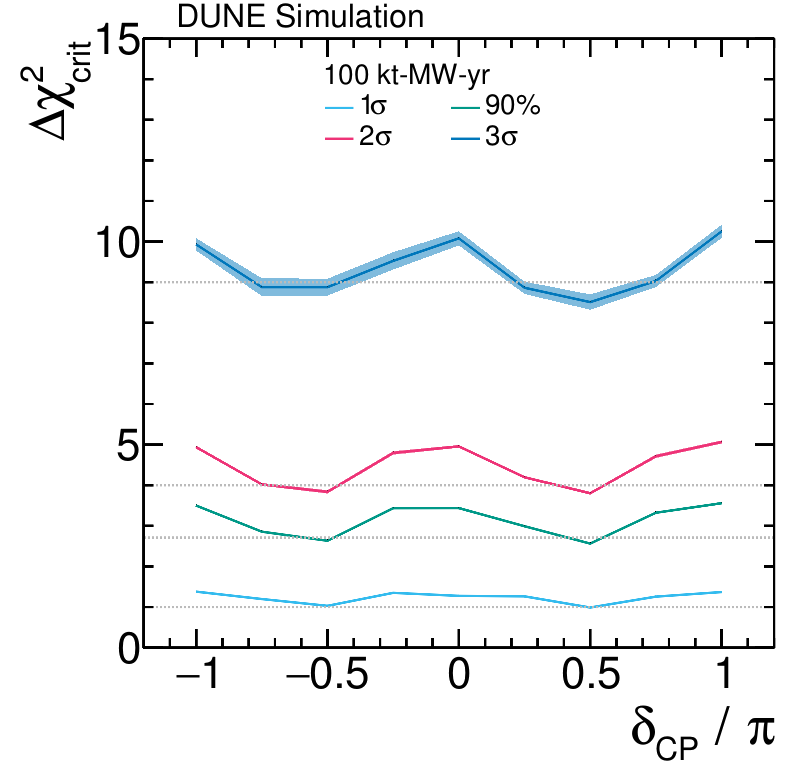
\includegraphics[width=0.8\columnwidth]{dchi2crit_vs_dcp_100ktMWyr.png}}\\
  \subfloat[334 ktMWyr]  {\label{fig:fc_vs_dcp_334}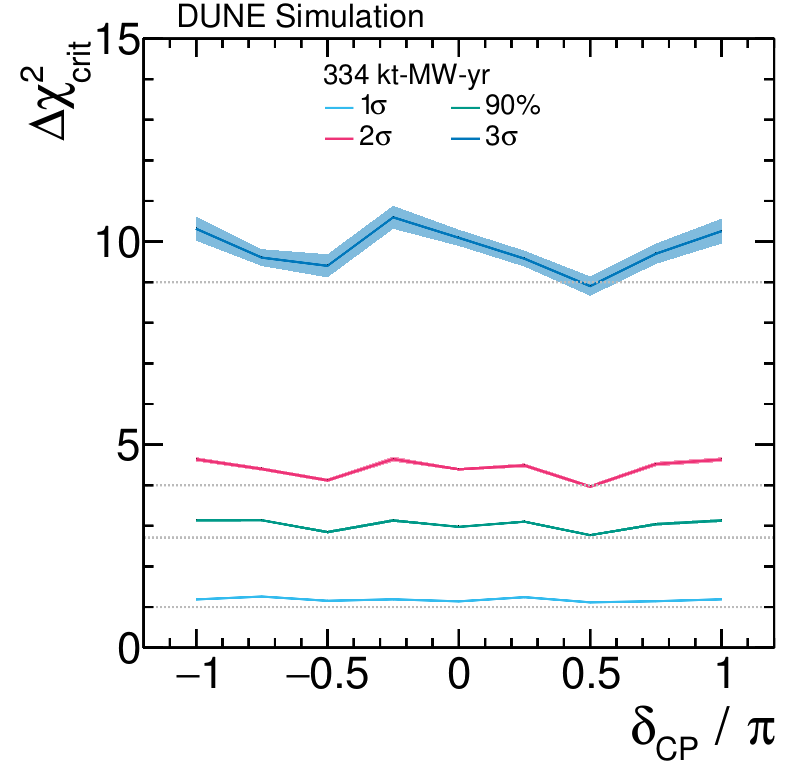
\includegraphics[width=0.8\columnwidth]{dchi2crit_vs_dcp_334ktMWyr.png}}
  \caption{The \dchisqcrit values corresponding to 68.27\% (1$\sigma$), 90\%, 95.45\% (2$\sigma$) and 99.73\% (3$\sigma$) of throws, shown as a function of true \deltacp, for exposures of 100 ktMWyr and 334 ktMWyr. The uncertainty on the \dchisqcrit values is obtained using Equation~\ref{eq:fc_uncertainty}, and is indicated as the shaded line. To guide the eye, horizontal dashed lines are included which indicate the 1$\sigma$, 90\%, 2$\sigma$ and 3$\sigma$ \dchisq values assumed using the constant-\dchisq method, with one degree of freedom. The distribution of throws used produced to calculate the \dchisqcrit values shown are given in Figure~\ref{fig:fc_throws_100ktMWyr} (Figure~\ref{fig:fc_throws_334ktMWyr}) for 100 ktMWyr (334 ktMWyr).}
  \label{fig:fc_vs_dcp}
\end{figure}
As \deltacp is a cyclical parameter, with physical boundaries at $\pm\pi$, it is interesting to see how the \dchisqcrit values evolve as a function of it. Figure~\ref{fig:fc_vs_dcp} shows the \dchisqcrit as a function of true \deltacp, for an ND+FD analysis with an equal FHC:RHC run fraction and a $\theta_{13}$ penalty applied, for 100 ktMWyr and 334 ktMWyr exposures. There is a noticeable, although not large, depression in the \dchisqcrit values at $\deltacp = \pm\pi/2$ for all significance levels considered. This effect is larger at the lower, 100 ktMWyr, exposure, and is larger at higher significance levels. It is also clear from Figure~\ref{fig:fc_vs_dcp} that the \dchisqcrit behaviour is very similar at $\delta = \pm\pi/2$ as at $\deltacp = 0$. Although the \dchisqcrit values are relevant for CPV sensitivity, this evolution of the \dchisqcrit values with \deltacp will be important for estimating DUNE's \deltacp resolution. Details on the number of toy throws used at each point of Figure~\ref{fig:fc_vs_dcp} are given in Appendix~\ref{sec:fc_appendix}, and the toy throw distributions are shown for the 100 ktMWyr (334 ktMWyr) test points in Figure~\ref{fig:fc_throws_100ktMWyr} (Figure~\ref{fig:fc_throws_334ktMWyr}).

\begin{figure*}[htbp]
  \centering
  \subfloat[24 ktMWyr]  {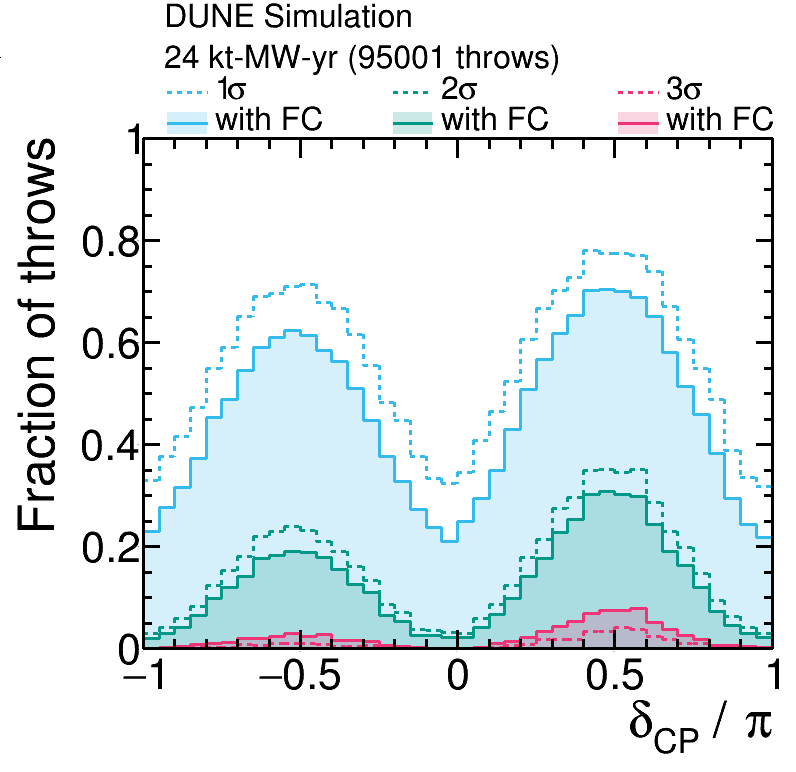
\includegraphics[width=0.33\linewidth]{cpv_throws_withFC_24ktMWyr_NH_th13.png}}
  \subfloat[66 ktMWyr]  {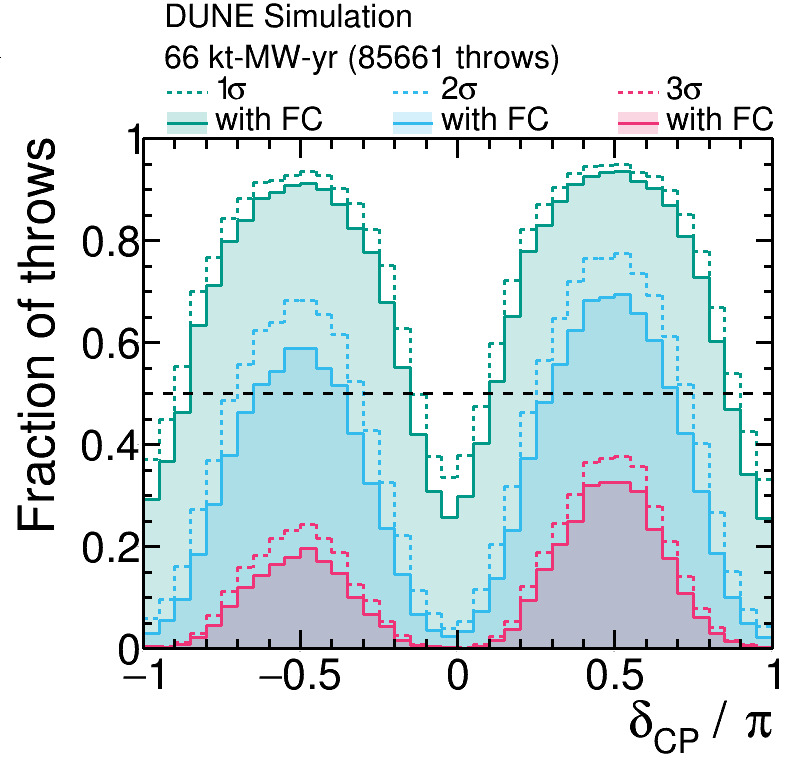
\includegraphics[width=0.33\linewidth]{cpv_throws_withFC_66ktMWyr_NH_th13.png}}
  \subfloat[100 ktMWyr] {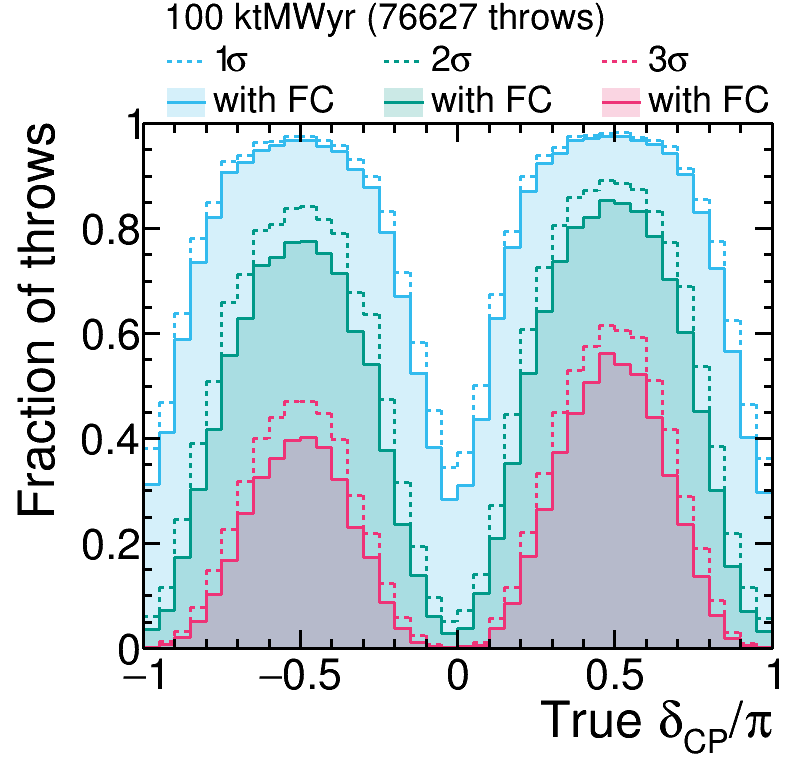
\includegraphics[width=0.33\linewidth]{cpv_throws_withFC_100ktMWyr_NH_th13.png}}\\
  \subfloat[150 ktMWyr] {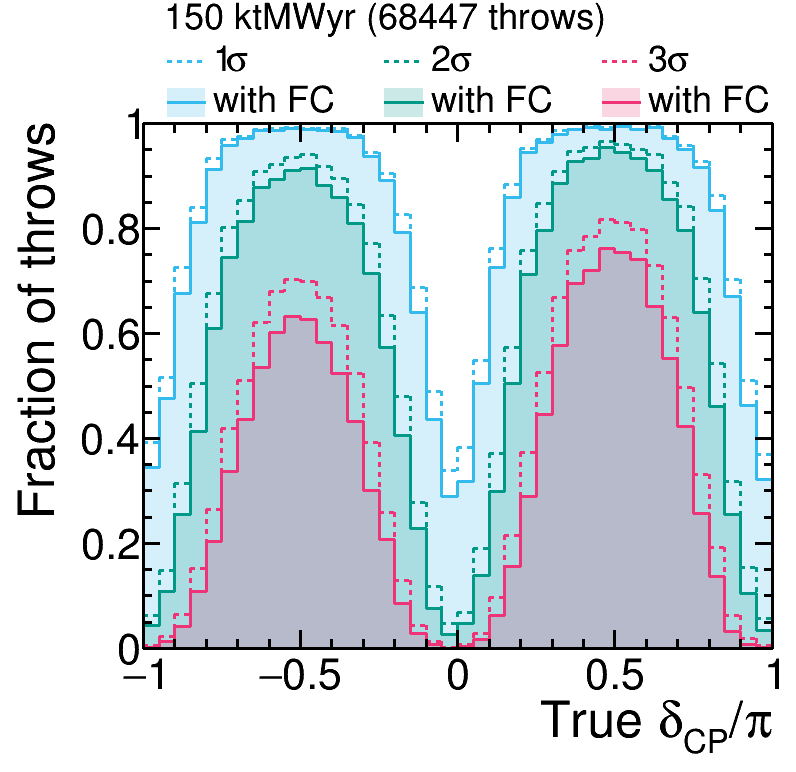
\includegraphics[width=0.33\linewidth]{cpv_throws_withFC_150ktMWyr_NH_th13.png}}
  \subfloat[197 ktMWyr] {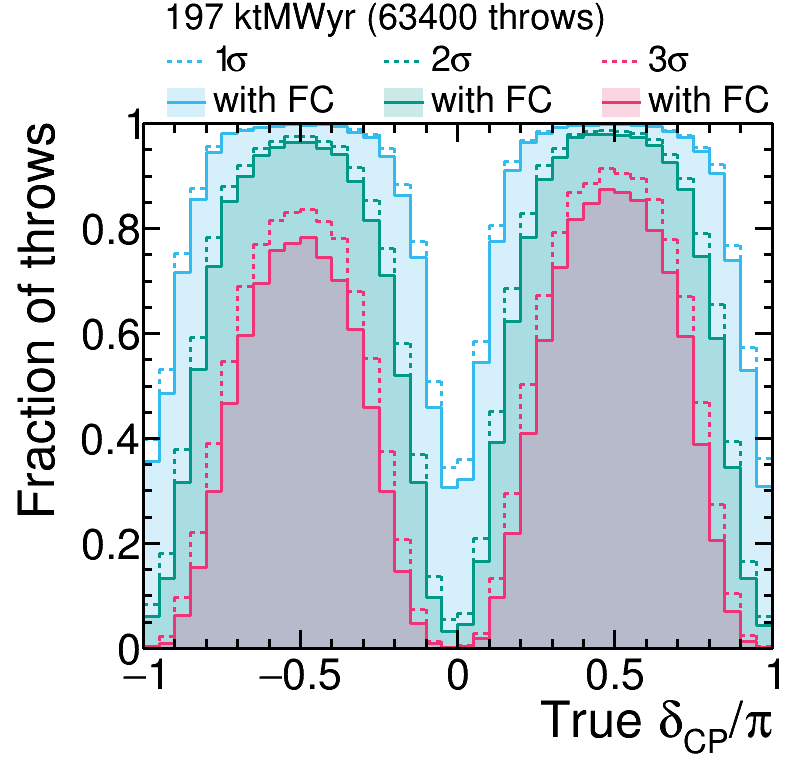
\includegraphics[width=0.33\linewidth]{cpv_throws_withFC_197ktMWyr_NH_th13.png}}
  \subfloat[334 ktMWyr] {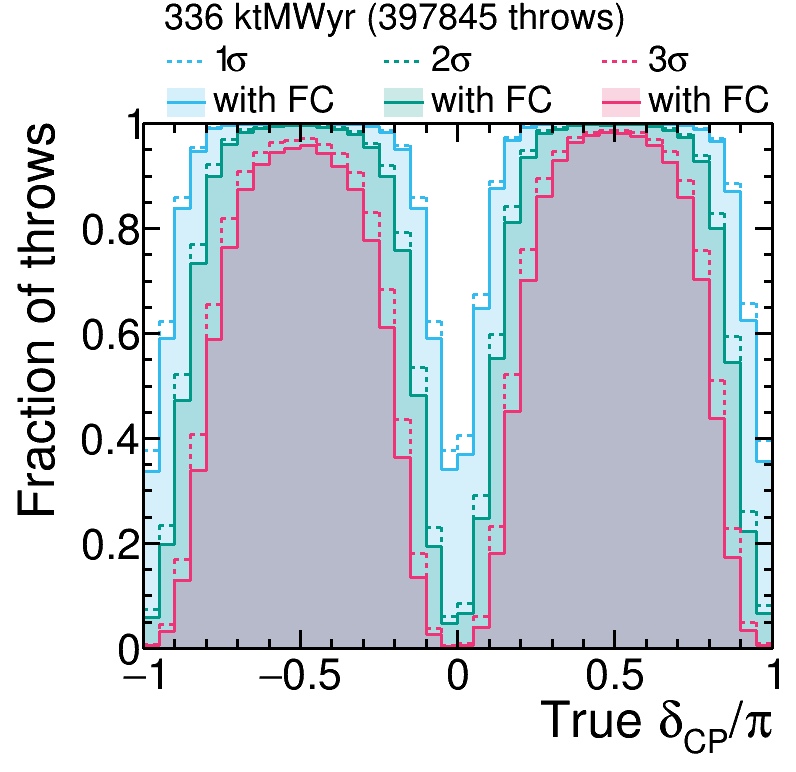
\includegraphics[width=0.33\linewidth]{cpv_throws_withFC_334ktMWyr_NH_th13.png}}
  \caption{Fraction of throws for which the DUNE sensitivity to CP-violation ($\deltacp \neq [0,\pm\pi]$) exceeds 1--3$\sigma$ significance, calculated using constant-\dchisq (dashed lines) and \dchisqcrit values calculated using the Feldman-Cousins method (shaded histograms), as a function of the true value of \deltacp. Shown for NO, for a number of different exposures. The number of throws used to make each figure is also shown.}
  \label{fig:cpv_over_time_fc}
\end{figure*}
Having calculated the \dchisqcrit values necessary to achieve correct coverage, it is possible to re-evaluate the CPV sensitivity previously shown assuming a constant \dchisq method in Figure~\ref{fig:cpv_over_time}. Figure~\ref{fig:cpv_over_time_fc} shows the 1, 2 and 3$\sigma$ CPV sensitivities as a function of true \deltacp, with and without the Feldman-Cousins correction (e.g., the \dchisqcrit values given in Figure~\ref{fig:fc_vs_exp} applied). The uncorrected values are the same as in Figure~\ref{fig:cpv_over_time}. In general, the effect of the Feldman-Cousins correction is to reduce the fraction of toy throws that cross each significance threshold, by a maximum of $\sim$10\%, but the eact fraction changes as a function of true \deltacp value and exposure. An exception to this general trend is the 3$\sigma$ behaviour at 24 ktMWyr, the lowest exposure shown, where the significance increases. This can be understood because of the rise in the 3$\sigma$ \dchisqcrit value at low exposures observed in Figure~\ref{fig:fc_vs_exp}.

\begin{figure*}[htbp]
  \centering
  \subfloat[$\deltacp = -\pi/2$] {\includegraphics[width=0.8\columnwidth]{{fraction_throws_vs_exp_dcp-0.5_FC}.pdf}}
  \subfloat[$\deltacp = +\pi/2$] {\includegraphics[width=0.8\columnwidth]{{fraction_throws_vs_exp_dcp0.5_FC}.pdf}}
  \caption{Fraction of throws for which the DUNE sensitivity to CP-violation ($\deltacp \neq [0,\pm\pi]$) exceeds 1--3$\sigma$ significance, at $\deltacp = \pm\pi/2$, calculated using constant-\dchisq (dashed lines) and \dchisqcrit values calculated using the Feldman-Cousins methed (shaded histograms), as a function of exposure.}
  \label{fig:cpv_vs_exp_fc}
\end{figure*}
Figure~\ref{fig:cpv_vs_exp_fc} shows the fraction of throws which exceed different significance thresholds at the maximal \deltacp violation values of $\pm\pi/2$, as a function of exposure, with and without Feldman-Cousins corrections, for 1--3$\sigma$ significance values. It is clear from Figure~\ref{fig:cpv_vs_exp_fc} that the effect of the correction is not large, and $\sim$10\% longer exposures are required for the median sensitivity to cross each significance threshold than without correction, at both points shown.

\FloatBarrier

\section{Neutrino mass ordering sensitivity}
\label{sec:mh_sens}

In this section, the toy-throwing approach described in Section~\ref{sec:analysis_framework} is used to explore the neutrino mass ordering sensitivity as a function of exposure in detail. In all cases, a joint ND+FD fit is performed, and the reactor $\theta_{13}$ constraint is always applied, as described in Section~\ref{sec:analysis_framework}. An equal split between FHC and RHC running is assumed based on the results obtained in Section~\ref{sec:run_plan_opt}.

\begin{figure}[htbp]
  \centering
  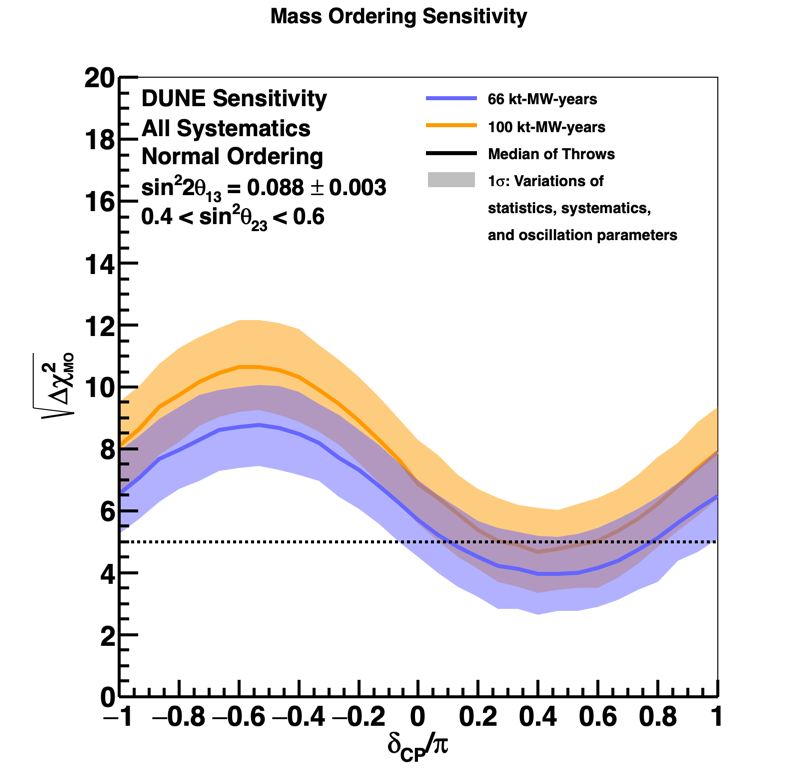
\includegraphics[width=0.8\linewidth, trim={0cm 0cm 0cm 2.3cm}, clip]{mh_two_exps_throws_nh_2019_v4_lowexp.png}
  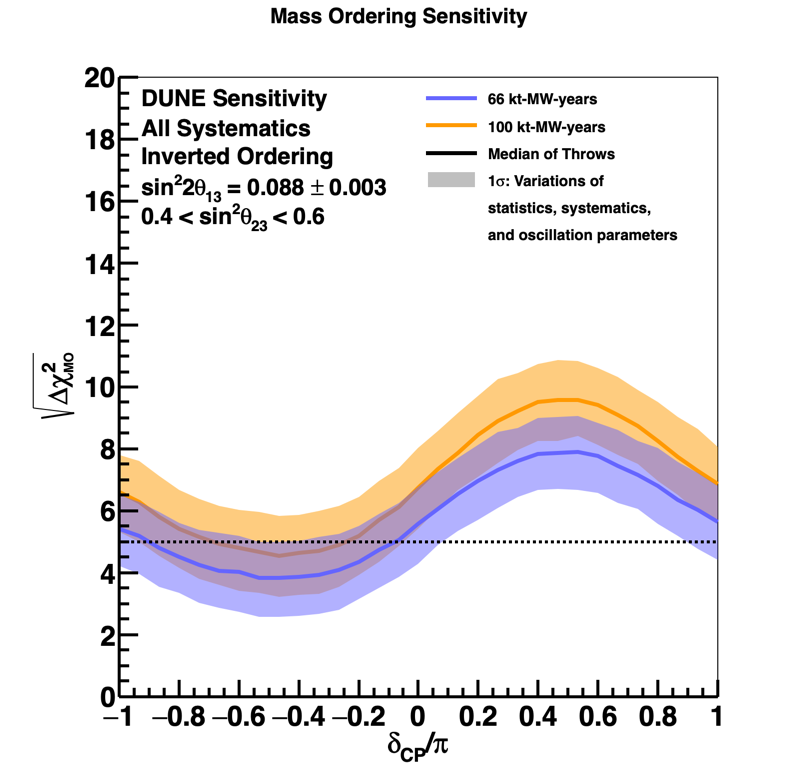
\includegraphics[width=0.8\linewidth, trim={0cm 0cm 0cm 2.3cm}, clip]{mh_two_exps_throws_ih_2019_v4_lowexp.png}
  \caption{Significance of the DUNE determination of the neutrino mass ordering, as a function of the true value of \deltacp, for 66 kt-MW-yrs (blue) and 100 kt-MW-yrs (orange) exposures. The width of the transparent bands cover 68\% of fits in which random throws are used to simulate systematic, oscillation parameter and statistical variations, with independent fits performed for each throw constrained by pre-fit uncertainties. The solid lines show the median significance.}
  \label{fig:mh_bands}
\end{figure}
Figure~\ref{fig:mh_bands} shows the significance with which the neutrino mass ordering can be determined for both true NO and IO, for exposures of 66 and 100 kt-MW-yrs. The sensitivity metric used is the square root of the difference between the best fit $\chi^{2}$ value obtained using each ordering, as shown in Equation~\ref{eq:mh_chi2}, which is calculated for each throw of the systematic, other oscillation parameters and statistics. The characteristic shape of the MH sensitivity in Figure~\ref{fig:mh_bands} results from near degeneracy between matter and CPV effects that occurs near $\deltacp=\pi/2$ ($-\deltacp=\pi/2$) for true normal (inverted) ordering. We note that dedicated studies have shown that special attention must be paid to the statistical interpretation of neutrino mass ordering sensitivities~\cite{Ciuffoli:2013rza,Qian:2012zn,Blennow:2013oma} because the \dchisq metric does not follow the expected chi-square distribution for one degree of freedom, so the interpretation of the $\sqrt{\dchisq}$ as the sensitivity is complicated.

\begin{figure*}[htbp]
  \centering
  \subfloat[6 kt-MW-yrs]   {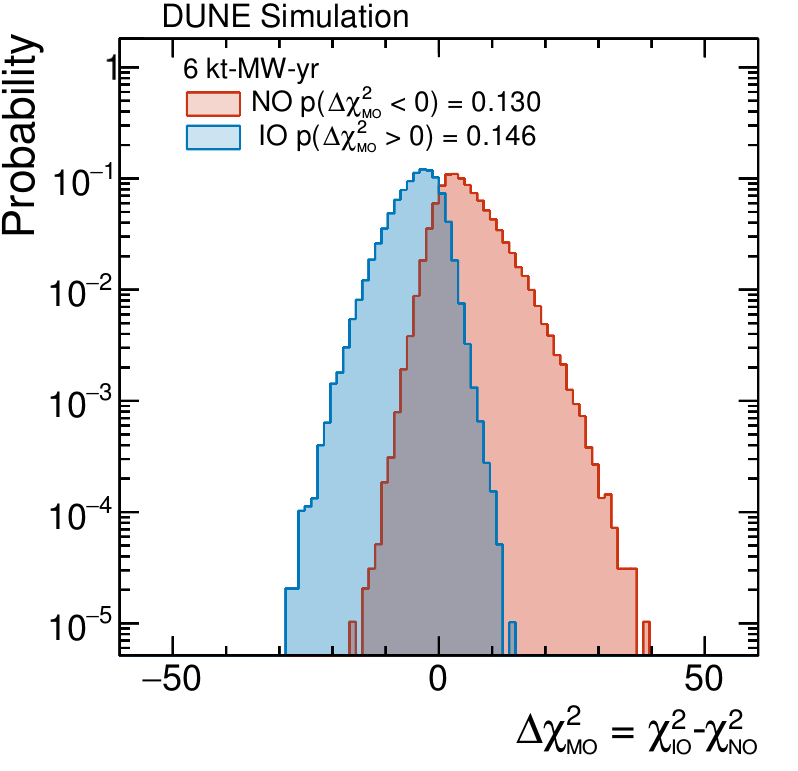
\includegraphics[width=0.33\linewidth]{MH_comp_ndfd_6ktMWyr_th13.png}}
  \subfloat[12 kt-MW-yrs]  {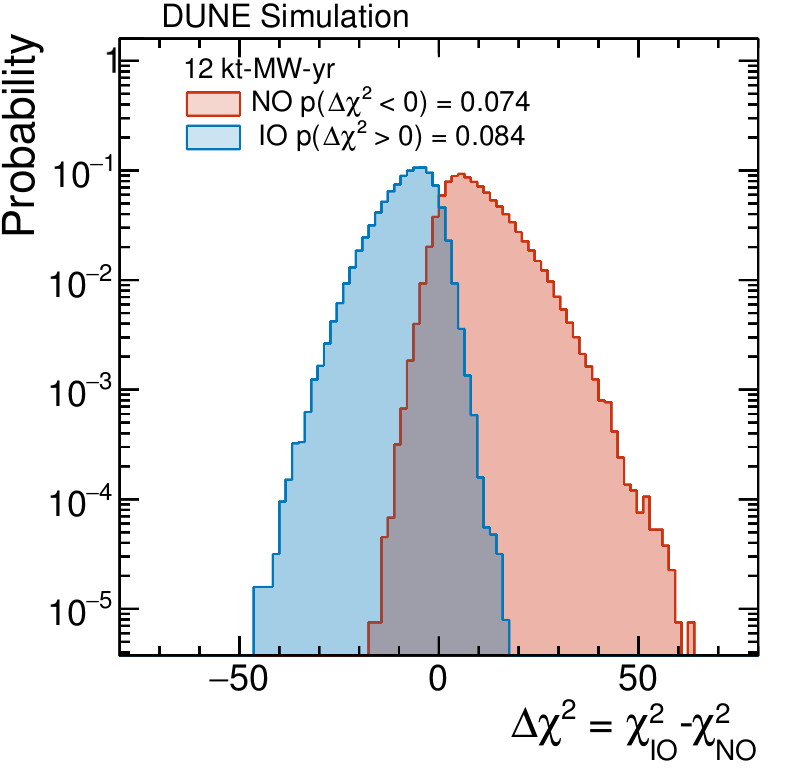
\includegraphics[width=0.33\linewidth]{MH_comp_ndfd_12ktMWyr_th13.png}}
  \subfloat[24 kt-MW-yrs]  {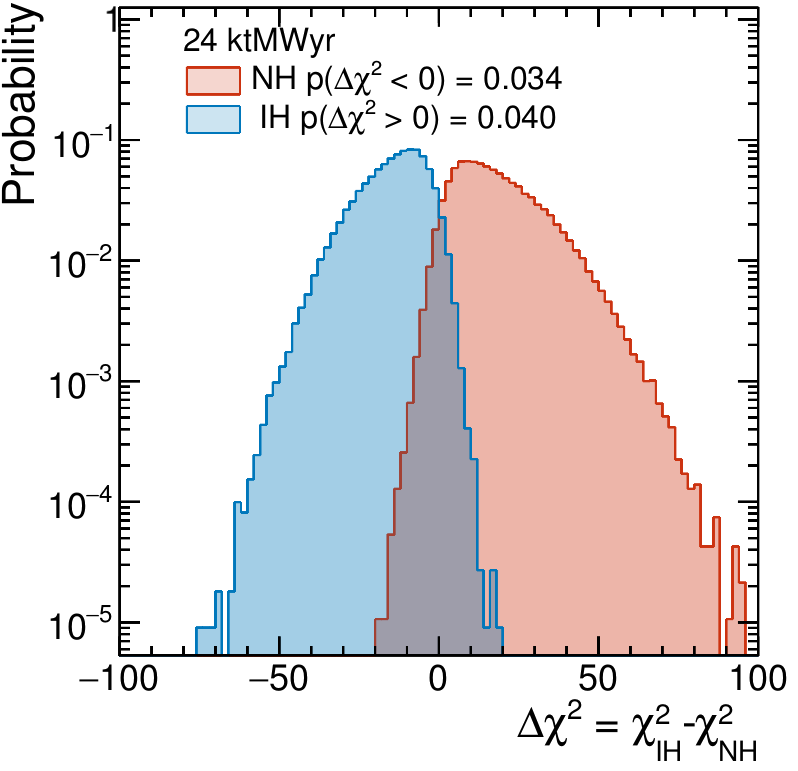
\includegraphics[width=0.33\linewidth]{MH_comp_ndfd_24ktMWyr_th13.png}}\\
  \subfloat[66 kt-MW-yrs]  {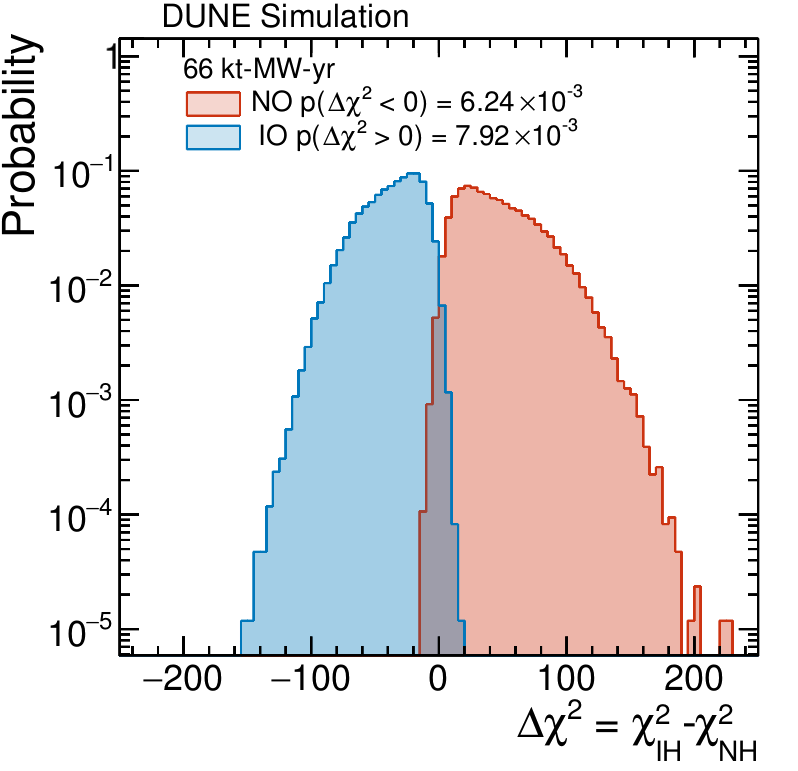
\includegraphics[width=0.33\linewidth]{MH_comp_ndfd_66ktMWyr_th13.png}}
  \subfloat[100 kt-MW-yrs] {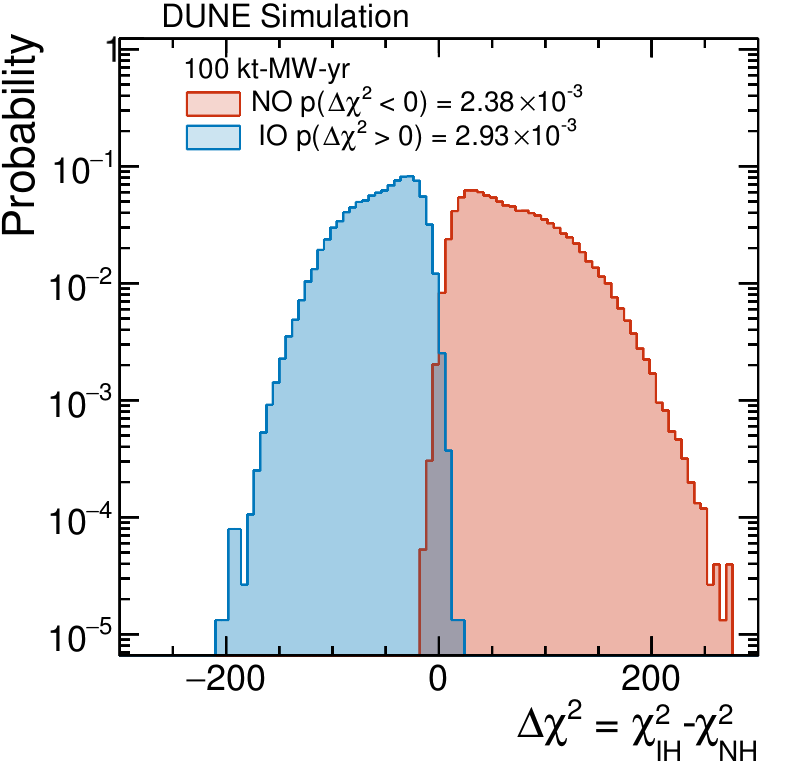
\includegraphics[width=0.33\linewidth]{MH_comp_ndfd_100ktMWyr_th13.png}}
  \subfloat[334 kt-MW-yrs] {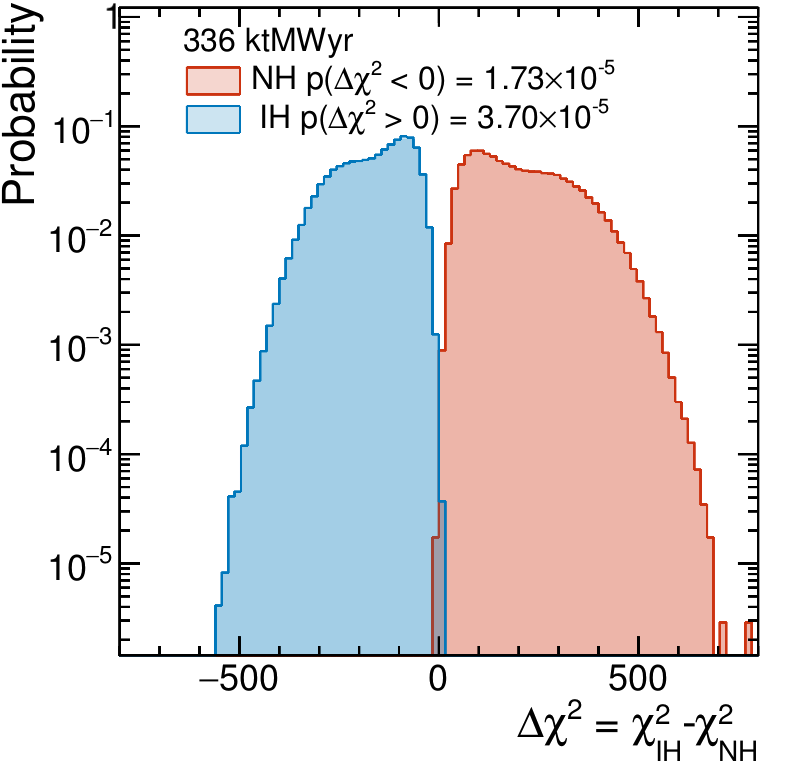
\includegraphics[width=0.33\linewidth]{MH_comp_ndfd_334ktMWyr_th13.png}}
  \caption{The distribution of $\dchisq = \chi^{2}_{\mathrm{IO}} - \chi^{2}_{\mathrm{NO}}$ values shown for both true normal (red) and true inverted (blue) hierarchies built using random throws of the systematic parameters, the oscillation parameters and with statistical variations. In each case, the $\chi^{2}$ values are separately minimized with respect to all variable parameters before calculating the test statistic. The fraction of throws for which the value of \dchisq is greater than (less than) 0 is also given for inverted (normal) hierarchies. For each ordering and exposure, approximately 100,000 throws were used.}
  \label{fig:mh_comp_over_time}
\end{figure*}
Given the complications with the interpretation of significance for mass ordering determination, it is instructive to look at the distribution of the test-statistic (Equation~\ref{eq:mh_chi2}), which gives more information than the 68\% central band and median throw shown in Figure~\ref{fig:mh_bands}. Figure~\ref{fig:mh_comp_over_time} shows the distribution of \dchisq obtained for a large ensemble of throws, for both true and inverted orderings, for a number of different exposures. Note that there is a uniform distribution of true \deltacp used in the throws at each exposure. The change in shape at higher exposures in Figure~\ref{fig:mh_comp_over_time} is due to the relationship with \deltacp, and as might be expected from Figure~\ref{fig:mh_bands}, the separation between hierarchies is greater for some true values of \deltacp than others. Note that this additional structure starts to become obvious from a $\sim$66 kt-MW-yrs exposure, at which point the CPV sensitivity is not very strong (see Section~\ref{sec:cp_sens}). For all exposures, the shape of the throw distribution is highly non-Gaussian, which makes it difficult to apply simple corrections to the sensitivity of the sort described in Ref.~\cite{Blennow:2013oma}. As a result we do not explore alternatives to $\sqrt{\dchisq}$ as a sensitivity metric, but note that the full information is given in Figure~\ref{fig:mh_comp_over_time}.

Figure~\ref{fig:mh_comp_over_time} also indicates the probability for the test statistic \dchisq to be less (more) than zero from the toy throws for true normal (inverted) hierarchies at each exposure. This marks the proportion of toys which appear more like the incorrect ordering than the true ordering for the toy. However, it is not easily converted to a single number sensitivity, although it does indicate the risk of a type I/type II error if the \dchisq value obtained by an experiment is exactly zero. It is clear from Figure~\ref{fig:mh_comp_over_time} that DUNE is sensitive to the mass ordering even from very low ($\sim$10 kt-MW-yrs) exposures, and by exposures of 66 kt-MW-yrs, the overlap between the orderings is very small.

\begin{figure*}[htbp]
  \centering
  \subfloat[6 kt-MW-yrs]   {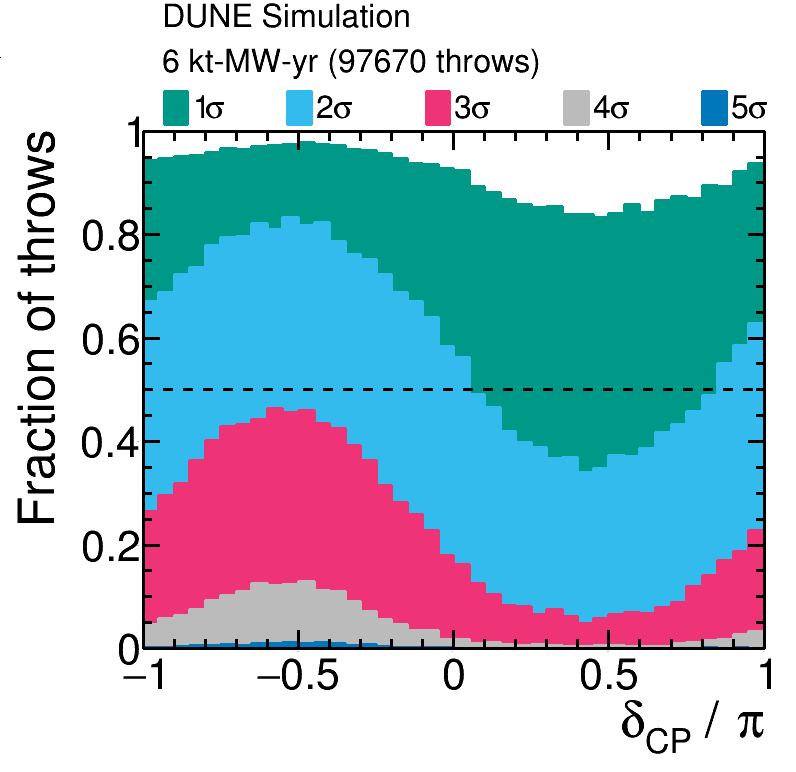
\includegraphics[width=0.33\linewidth]{mh_throws_6ktMWyr_NH_th13.png}}
  \subfloat[12 kt-MW-yrs]  {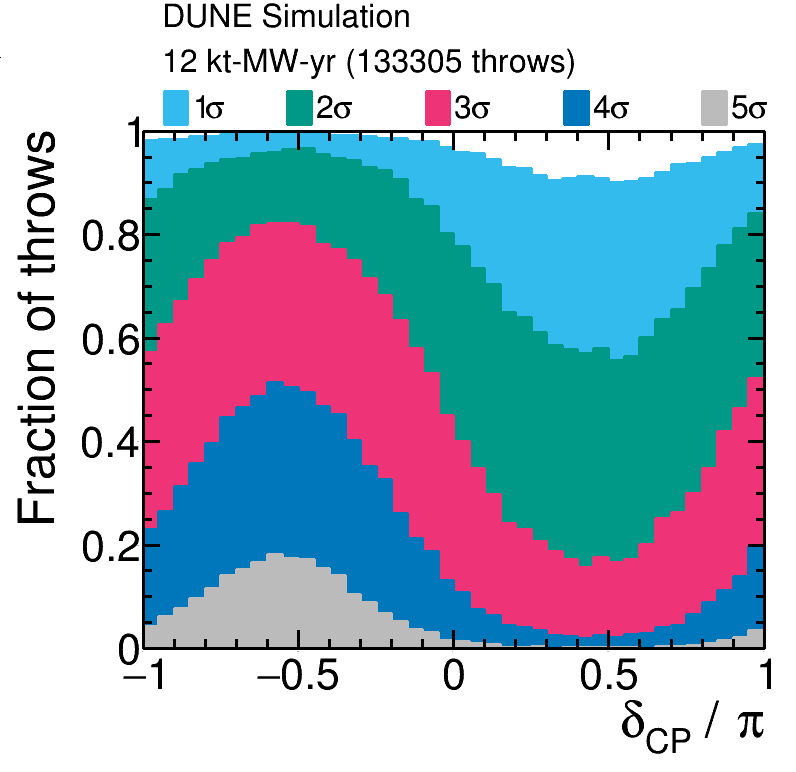
\includegraphics[width=0.33\linewidth]{mh_throws_12ktMWyr_NH_th13.png}}
  \subfloat[24 kt-MW-yrs]  {\includegraphics[width=0.33\linewidth]{mh_throws_24ktMWyr_NH_th13.png}}\\
  \subfloat[66 kt-MW-yrs]  {\includegraphics[width=0.33\linewidth]{mh_throws_66ktMWyr_NH_th13.png}}
  \subfloat[100 kt-MW-yrs] {\includegraphics[width=0.33\linewidth]{mh_throws_100ktMWyr_NH_th13.png}}
  \subfloat[334 kt-MW-yrs] {\includegraphics[width=0.33\linewidth]{mh_throws_334ktMWyr_NH_th13.png}}
  \caption{Fraction of throws for which the DUNE sensitivity to the mass ordering exceeds 1--5$\sigma$ significance, as a function of the true value of \deltacp. Shown for NO, for a number of different exposures. The number of throws used to make each figure is also shown.}
  \label{fig:mh_nh_over_time}
\end{figure*}

Figure~\ref{fig:mh_nh_over_time} shows an alternative way to present the result of the throws as a function of \deltacp, which is complementary to Figure~\ref{fig:mh_bands}. The fraction of throws for which the simple figure of merit (the square-root of Equation~\ref{eq:mh_chi2}) exceeds different confidence levels are shown, for 1--5$\sigma$ significances, and a variety of exposures, all for true NO. The same throws are used as in Figures~\ref{fig:mh_comp_over_time}. The highest exposure shown, 334 kt-MW-yrs, corresponds to the seven-year exposure using the nominal staging scenario in Ref.~\cite{Abi:2020qib}. Despite the caveats regarding the intepretation of $\sqrt{\dchisq}$ as units of $\sigma$, the general trend is clear, and provides more information about the expected DUNE sensitivity at low exposures. As with Figure~\ref{fig:cpv_over_time}, the point at which the median significance (50\% of throws) passes different significance thresholds can be easily read from the figures, and can be compared with those shown in Figure~\ref{fig:mh_bands}. The same general shape as a function of \deltacp as was observed in Figure~\ref{fig:mh_bands} can be seen. The general trend would be very similar in IO, reflected in the line $\deltacp = 0$. The median significance for $\deltacp = -\pi/2$ exceeds 5$\sigma$ for 24 kt-MW-yrs, at which point the fraction of throws for which the significance is 3$\sigma$ or greater is small, $\sim$2\%. By 66 kt-MW-yrs, 100\% of the throws exceed 5$\sigma$ at $\deltacp = -\pi/2$. By 100 kt-MW-yrs exposures, the median significance for all true values of \deltacp exceeds 5$\sigma$. At long exposures of 334 kt-MW-yrs, almost 100\% of the throws exceed 5$\sigma$ for all values of \deltacp.

\section{Conclusion}
\label{sec:conclude}

In this work we have presented a detailed exploration of DUNE's sensitivity to CPV and the mass ordering at low exposures. The analysis uses the same framework, flux, cross section and detector models and selections as were used in Ref.~\cite{Abi:2020qib}, which showed the ultimate DUNE sensitivity to CPV, MO and other oscillation parameters, with large statistics samples after long exposures.

\todo{Add comment about run plan optimization...}

The studies presented here demonstrate that a full treatment of DUNE's sensitivity at low exposures supports the conclusions made in Refs.~\cite{Abi:2020qib} and~\cite{Abi:2020evt} using simple Asimov studies. In particular, the median CPV sensitivity is $\sim$3$\sigma$ for $\deltacp = \pm\pi/2$ after approximately a 100 ktMWyr FD exposure. We also explore the variations in the expected sensitivity around the median value. Additionally, we show that the CPV sensitivity is not significantly degraded when Feldman-Cousins corrections are included, leading to $\sim$10\% longer exposures to reach a given significance level. Crucially, we find that after an initial low-exposure rise, the Feldman-Cousins \dchisqcrit do not change as a function of exposure, as has been observed by the T2K experiment~\cite{Abe:2021gky}.

We have also shown that strong statements on the mass ordering can be expected with very short exposures of $\sim$12 ktMWyr, which supports the results shown in Refs.~\cite{Abi:2020qib} and~\cite{Abi:2020evt} with a more complete treatment of the systematic uncertainty.

We note that although the analysis used here makes no assumptions about the FD staging scenario, and results are given as a function of exposure only, the results are dependent on having a performant ND complex from the start of the experiment. In particular, the low-exposures necessary to make world-leading statements about the mass hierarchy can only be given with confidence with ND samples included in the fit. We note also that additional samples of events from other detectors in the DUNE ND complex are not explicitly included in this analysis, but there is an assumption that we will be able to control the uncertainties to the level used in the analysis, and it should be understood that that implicitly relies on having a highly capable ND.

\begin{acknowledgements}
This document was prepared by the DUNE collaboration using the
resources of the Fermi National Accelerator Laboratory 
(Fermilab), a U.S. Department of Energy, Office of Science, 
HEP User Facility. Fermilab is managed by Fermi Research Alliance, 
LLC (FRA), acting under Contract No. DE-AC02-07CH11359.
%
% Funding agencies, alphabetical by country, then alphabetical by agency name
%
This work was supported by
CNPq,
FAPERJ,
FAPEG and 
FAPESP,                         Brazil;
CFI, 
IPP and 
NSERC,                          Canada;
CERN;
M\v{S}MT,                       Czech Republic;
ERDF, 
H2020-EU and 
MSCA,                           European Union;
CNRS/IN2P3 and
CEA,                            France;
INFN,                           Italy;
FCT,                            Portugal;
NRF,                            South Korea;
CAM, 
Fundaci\'{o}n ``La Caixa'',
Junta de Andaluc\'ia-FEDER, and 
MICINN,                         Spain;
SERI and 
SNSF,                           Switzerland;
T\"UB\.ITAK,                    Turkey;
The Royal Society and 
UKRI/STFC,                      United Kingdom;
DOE and 
NSF,                            United States of America.
This research used resources of the 
National Energy Research Scientific Computing Center (NERSC), 
a U.S. Department of Energy Office of Science User Facility 
operated under Contract No. DE-AC02-05CH11231.
\end{acknowledgements}

\bibliographystyle{utphys}
\bibliography{tdr-citedb}

\appendix*
\section{Feldman-Cousins throw distributions}\label{sec:fc_appendix}

\begin{figure*}[htbp]
  \centering
  \subfloat[24 ktMWyr] {\includegraphics[width=0.33\linewidth]{nh_FC_ndfd_24ktMWyr_dcp0.png}}
  \subfloat[66 ktMWyr] {\includegraphics[width=0.33\linewidth]{nh_FC_ndfd_66ktMWyr_dcp0.png}}
  \subfloat[100 ktMWyr]{\includegraphics[width=0.33\linewidth]{nh_FC_ndfd_100ktMWyr_dcp0.png}}\\
  \subfloat[150 ktMWyr]{\includegraphics[width=0.33\linewidth]{nh_FC_ndfd_150ktMWyr_dcp0.png}}
  \subfloat[197 ktMWyr]{\includegraphics[width=0.33\linewidth]{nh_FC_ndfd_197ktMWyr_dcp0.png}}
  \subfloat[336 ktMWyr]{\includegraphics[width=0.33\linewidth]{nh_FC_ndfd_334ktMWyr_dcp0.png}}\\
  \subfloat[500 ktMWyr]{\includegraphics[width=0.33\linewidth]{nh_FC_ndfd_500ktMWyr_dcp0.png}}
  \subfloat[646 ktMWyr]{\includegraphics[width=0.33\linewidth]{nh_FC_ndfd_646ktMWyr_dcp0.png}}
  \subfloat[936 ktMWyr]{\includegraphics[width=0.33\linewidth]{nh_FC_ndfd_936ktMWyr_dcp0.png}}
  \caption[]{}
  \label{fig:fc_throws_exp}
\end{figure*}

\begin{figure*}[htbp]
  \centering
  \subfloat[$\deltacp/\pi = -1$]    {\includegraphics[width=0.33\linewidth]{{nh_FC_ndfd_100ktMWyr_dcp-1}.png}}
  \subfloat[$\deltacp/\pi = -0.75$] {\includegraphics[width=0.33\linewidth]{{nh_FC_ndfd_100ktMWyr_dcp-0.75}.png}}
  \subfloat[$\deltacp/\pi = -0.5$]  {\includegraphics[width=0.33\linewidth]{{nh_FC_ndfd_100ktMWyr_dcp-0.5}.png}}\\
  \subfloat[$\deltacp/\pi = -0.25$] {\includegraphics[width=0.33\linewidth]{{nh_FC_ndfd_100ktMWyr_dcp-0.25}.png}}
  \subfloat[$\deltacp/\pi = 0$]     {\includegraphics[width=0.33\linewidth]{{nh_FC_ndfd_100ktMWyr_dcp0}.png}}
  \subfloat[$\deltacp/\pi = 0.25$]  {\includegraphics[width=0.33\linewidth]{{nh_FC_ndfd_100ktMWyr_dcp0.25}.png}}\\
  \subfloat[$\deltacp/\pi = 0.5$]   {\includegraphics[width=0.33\linewidth]{{nh_FC_ndfd_100ktMWyr_dcp0.5}.png}}
  \subfloat[$\deltacp/\pi = 0.75$]  {\includegraphics[width=0.33\linewidth]{{nh_FC_ndfd_100ktMWyr_dcp0.75}.png}}
  \subfloat[$\deltacp/\pi = 1$]     {\includegraphics[width=0.33\linewidth]{{nh_FC_ndfd_100ktMWyr_dcp1}.png}}
  \caption[]{}
  \label{fig:fc_throws_100ktMWyr}
\end{figure*}

\begin{figure*}[htbp]
  \centering
  \subfloat[$\deltacp/\pi = -1$]    {\includegraphics[width=0.33\linewidth]{{nh_FC_ndfd_334ktMWyr_dcp-1}.png}}
  \subfloat[$\deltacp/\pi = -0.75$] {\includegraphics[width=0.33\linewidth]{{nh_FC_ndfd_334ktMWyr_dcp-0.75}.png}}
  \subfloat[$\deltacp/\pi = -0.5$]  {\includegraphics[width=0.33\linewidth]{{nh_FC_ndfd_334ktMWyr_dcp-0.5}.png}}\\
  \subfloat[$\deltacp/\pi = -0.25$] {\includegraphics[width=0.33\linewidth]{{nh_FC_ndfd_334ktMWyr_dcp-0.25}.png}}
  \subfloat[$\deltacp/\pi = 0$]     {\includegraphics[width=0.33\linewidth]{{nh_FC_ndfd_334ktMWyr_dcp0}.png}}
  \subfloat[$\deltacp/\pi = 0.25$]  {\includegraphics[width=0.33\linewidth]{{nh_FC_ndfd_334ktMWyr_dcp0.25}.png}}\\
  \subfloat[$\deltacp/\pi = 0.5$]   {\includegraphics[width=0.33\linewidth]{{nh_FC_ndfd_334ktMWyr_dcp0.5}.png}}
  \subfloat[$\deltacp/\pi = 0.75$]  {\includegraphics[width=0.33\linewidth]{{nh_FC_ndfd_334ktMWyr_dcp0.75}.png}}
  \subfloat[$\deltacp/\pi = 1$]     {\includegraphics[width=0.33\linewidth]{{nh_FC_ndfd_334ktMWyr_dcp1}.png}}
  \caption[]{}
  \label{fig:fc_throws_334ktMWyr}
\end{figure*}


\end{document}
